% ------------------------------------------------------------------------------
% ---------------------------------  LICENSE  ----------------------------------
% ------------------------------------------------------------------------------
% Except where otherwise noted, this work by Noita Enola is licensed under CC BY-SA 4.0. You can check a copy of the license by looking at the LICENSE.md file, or at <https://creativecommons.org/licenses/by-sa/4.0>.

% ------------------------------------------------------------------------------
% ---------------------------------   CLASS    ---------------------------------
% ------------------------------------------------------------------------------
\documentclass[%
	a5paper,
	10pt,
	twoside,
	openright,
%	draft,
	final,
]{memoir}

% ------------------------------------------------------------------------------
% ---------------------------------  COMMANDS  ---------------------------------
% ------------------------------------------------------------------------------
% ------------------------------------------------------------------------------
% ---------------------------------  LICENSE  ----------------------------------
% ------------------------------------------------------------------------------
% Except where otherwise noted, this work by Noita Enola is licensed under CC BY-SA 4.0. You can check a copy of the license by looking at the LICENSE.md file, or at <https://creativecommons.org/licenses/by-sa/4.0>.

% ------------------------------------------------------------------------------
% -------------------------------    COMMANDS    -------------------------------
% ------------------------------------------------------------------------------
% Some title/author commands
\newcommand{\documentTitle}{ScanManual/Guía para aprender a escanear}
\newcommand{\documentVersion}{v1.1}
\newcommand{\documentAuthor}{Noita Enola}
\newcommand{\documentURL}{https://github.com/Noitaenola/ScanManual}

% ------------------------------------------------------------------------------
% Text macros
\usepackage{xspace} % To manage spaces at the end of text macros

\newcommand{\pdf}{\textsc{pdf}\xspace}
\newcommand{\pdfa}{\textsc{pdf/a}\xspace}
\newcommand{\djvu}{\textsc{djvu}\xspace}
\newcommand{\tiff}{\textsc{tiff}\xspace}
\newcommand{\png}{\textsc{png}\xspace}
\newcommand{\jpeg}{\textsc{jpeg}\xspace}
\newcommand{\jbig}{\textsc{jbig}\xspace}
\newcommand{\adf}{\textsc{adf}\xspace}
\newcommand{\ocr}{\textsc{ocr}\xspace}
\newcommand{\mondaytwothousand}{monday2000\xspace} % Acoording to a footnote at http://www.djvu-soft.narod.ru/ this grumpy old guy is called Ivanov Victor (Иванов Виктор). He dissapears from the scene around 2014.
\newcommand{\textsharik}{textsharik\xspace}

\newcommand{\szip}{\textsc{7-Zip}\xspace}
\newcommand{\scantailor}{\textsc{Scan Tailor}\xspace}
\newcommand{\scantailorAdvanced}{\textsc{Scan Tailor Advanced}\xspace}
\newcommand{\irfanview}{\textsc{IrfanView}\xspace}
\newcommand{\xnview}{\textsc{XnView}\xspace}
\newcommand{\gimp}{\textsc{gimp}\xspace}
\newcommand{\abbyy}{\textsc{FineReader}\xspace}
\newcommand{\acrobat}{\textsc{Acrobat DC}\xspace}
\newcommand{\qpdf}{\textsc{qpdf}\xspace}
\newcommand{\veraPDF}{\textsc{veraPDF}\xspace}
\newcommand{\pdg}{\textsc{PdgCntEditor}\xspace}
\newcommand{\djvulibre}{\textsc{DjVuLibre}\xspace}
\newcommand{\dexpress}{\textsc{Document Express}\xspace}
\newcommand{\djvueditor}{\textsc{DjVu Editor}\xspace}
\newcommand{\djvusmall}{\textsc{DjVu Small}\xspace}
\newcommand{\djvusmallmod}{\textsc{DjVu Small Mod}\xspace}
\newcommand{\djvuimager}{\textsc{DjVu Imager}\xspace}
\newcommand{\notepad}{\textsc{Notepad\!+\!+}\xspace}
\newcommand{\imagemagick}{\textsc{ImageMagick}\xspace}
\newcommand{\exiftool}{\textsc{ExifTool}\xspace}

% ------------------------------------------------------------------------------
% Play icon
\newcommand{\play}{%
	\begin{tikzpicture}[baseline=-0.6ex]%
%		\node[circle, draw, thick, green!75!black, inner sep=3.2pt] (bcircle) {}; % This line draw the circle
		\node (bcircle) {}; % This one won't
		\node[scale=0.7, green!75!black, inner sep=0pt] at ([xshift=0.6pt] bcircle.center) {\faPlay};%
	\end{tikzpicture}%
}

% ------------------------------------------------------------------------------
% Bold plus-minus
\newcommand{\boldpm}{%
	\begin{tikzpicture}[baseline=-0.6ex]%
		\node (bcircle) {};%
		\node[inner sep=0pt] at ([yshift=.1em] bcircle.center) {\faPlus};%
		\node[inner sep=0pt] at ([yshift=-0.4em] bcircle.center) {\faMinus};%
	\end{tikzpicture}%
}

% ------------------------------------------------------------------------------
% Mouse click icons
\newcommand{\leftclick}{\raisebox{-.15em}{\!
\includegraphics[width=1em]{leftclick}}}
\newcommand{\rightclick}{\raisebox{-.15em}{\,
\includegraphics[width=1em]{rightclick}}}

% ------------------------------------------------------------------------------
% menukeys package commands with fontawesome5 icons

% ------------------------------------------------------------------------------
% typesetFile command
\newcommand{\typesetFile}[1]{%
	\faFile[regular]%
	\,%
	\directory{#1}%
}

% ------------------------------------------------------------------------------
% typesetExe command
\newcommand{\typesetExe}[1]{%
	\faFile*[regular]%
	\,%
	\directory{#1}%
}

% ------------------------------------------------------------------------------
% typesetFolder command
\newcommand{\typesetFolder}[1]{%
	\faFolderOpen[regular]%
	\,%
	\directory{#1}%
}

% ------------------------------------------------------------------------------
% typesetCheckbox command
\newcommand{\typesetCheckbox}[1]{%
	\faCheckSquare[regular]%
	\,%
	#1%
}

% ------------------------------------------------------------------------------
% typesetBox command
\newcommand{\typesetBox}[1]{%
	\faSquare[regular]%
	\,%
	#1%
}

% ------------------------------------------------------------------------------
% typesetCircle command
\newcommand{\typesetCircle}[1]{%
	\faCircle[regular]%
	\,%
	#1%
}

% ------------------------------------------------------------------------------
% typesetDotCircle command
\newcommand{\typesetDotCircle}[1]{%
	\faDotCircle[regular]%
	\,%
	#1%
}

% ------------------------------------------------------------------------------
% License command
\newcommand{\license}{
	\vspace{\baselineskip}
	\hfill%
	\begin{minipage}[c]{.35\linewidth}
		\doclicenseImage[imagewidth=\linewidth]\\\centering
		\doclicenseNameRef
	\end{minipage}
}


% ------------------------------------------------------------------------------
% ---------------------------------  PACKAGES  ---------------------------------
% ------------------------------------------------------------------------------
% ------------------------------------------------------------------------------
% ---------------------------------  LICENSE  ----------------------------------
% ------------------------------------------------------------------------------
% Except where otherwise noted, this work by Noita Enola is licensed under CC BY-SA 4.0. You can check a copy of the license by looking at the LICENSE.md file, or at <https://creativecommons.org/licenses/by-sa/4.0>.

% ------------------------------------------------------------------------------
% Font encoding
\usepackage[T1]{fontenc}
\usepackage[utf8]{inputenc}

% ------------------------------------------------------------------------------
% Font packages
\usepackage{fontawesome5} % various font icons
\usepackage[scaled=0.85]{beramono} % monospaced font
\usepackage{arev} % sans serif font
\usepackage{charter} % serif font
%\usepackage[scaled]{berasans} % alternative sans serif font

% The following lines fix the ligature selection problem with the libertine font. Source: https://tex.stackexchange.com/questions/4397/make-ligatures-in-linux-libertine-copyable-and-searchable
\input{glyphtounicode}
	\pdfglyphtounicode{f_f}{FB00}
	\pdfglyphtounicode{f_f_i}{FB03}
	\pdfglyphtounicode{f_f_l}{FB04}
	\pdfglyphtounicode{f_i}{FB01}
	\pdfgentounicode=1

% ------------------------------------------------------------------------------
% Localization
\usepackage[spanish]{babel}

% ------------------------------------------------------------------------------
% Microtypography
\usepackage[final]{microtype}

% ------------------------------------------------------------------------------

% ------------------------------------------------------------------------------
% ---------------------------------  LICENSE  ----------------------------------
% ------------------------------------------------------------------------------
% Except where otherwise noted, this work by Noita Enola is licensed under CC BY-SA 4.0. You can check a copy of the license by looking at the LICENSE.md file, or at <https://creativecommons.org/licenses/by-sa/4.0>.

% ------------------------------------------------------------------------------
% Thicker rulers
\let\oldtoprule\toprule
\renewcommand\toprule{\oldtoprule[1pt]}

\let\oldbottomrule\bottomrule
\renewcommand\bottomrule{\oldbottomrule[1pt]}
% ------------------------------------------------------------------------------

% ------------------------------------------------------------------------------
% ---------------------------------  LICENSE  ----------------------------------
% ------------------------------------------------------------------------------
% Except where otherwise noted, this work by Noita Enola is licensed under CC BY-SA 4.0. You can check a copy of the license by looking at the LICENSE.md file, or at <https://creativecommons.org/licenses/by-sa/4.0>.

% ------------------------------------------------------------------------------
\usepackage{graphicx}
	\graphicspath{{img/}} % images folder

% ------------------------------------------------------------------------------
\usepackage[table]{xcolor}

% ------------------------------------------------------------------------------
\usepackage{tikz}
	\usetikzlibrary{babel}

% ------------------------------------------------------------------------------

% ------------------------------------------------------------------------------
% ---------------------------------  LICENSE  ----------------------------------
% ------------------------------------------------------------------------------
% Except where otherwise noted, this work by Noita Enola is licensed under CC BY-SA 4.0. You can check a copy of the license by looking at the LICENSE.md file, or at <https://creativecommons.org/licenses/by-sa/4.0>.

% ------------------------------------------------------------------------------
% Barely used for a couple fractions
\usepackage{amsmath}

% ------------------------------------------------------------------------------

% ------------------------------------------------------------------------------
% ---------------------------------  LICENSE  ----------------------------------
% ------------------------------------------------------------------------------
% Except where otherwise noted, this work by Noita Enola is licensed under CC BY-SA 4.0. You can check a copy of the license by looking at the LICENSE.md file, or at <https://creativecommons.org/licenses/by-sa/4.0>.

% ------------------------------------------------------------------------------
% These two speed up compilation time but produce a larger PDF. Should be commented before doing the final build: https://tex.stackexchange.com/a/454235
\pdfcompresslevel=0
\pdfobjcompresslevel=0

% ------------------------------------------------------------------------------
% Depth of the bookmarks
\setsecnumdepth{subsubsection}
\settocdepth{section}

% ------------------------------------------------------------------------------
% ToDo notes in the margins
\usepackage[textsize=scriptsize]{todonotes}
	\setlength{\marginparwidth}{2cm}

% ------------------------------------------------------------------------------
% Sections of text in multiple columns
\usepackage{multicol}
% ------------------------------------------------------------------------------
% To ease customizing of the list environments
\usepackage{enumitem}

% ------------------------------------------------------------------------------
% hyperref package and hypelinks colour
\colorlet{colorLinks}{blue!30!black}

\usepackage[
	bookmarks,
	bookmarksopen,
	bookmarksdepth = 3,
	bookmarksopenlevel = 1,
	bookmarksnumbered,
%	hidelinks,
	colorlinks,
	allcolors=colorLinks,
	pdfusetitle,
	pdfview = Fit,
	pdfpagelayout = TwoPageRight,
]{hyperref}

% ------------------------------------------------------------------------------
% To typeset code snippets
\usepackage[newfloat]{minted}
\usepackage[skins, breakable, minted]{tcolorbox}
	\colorlet{bg}{black!5!white} % background color for snippets
%	\definecolor{bg}{rgb}{0.95,0.95,0.95}
	\newcommand{\pythonScript}[1]{% Shortcut for inputing scripts
		\begin{tcolorbox}[%
			arc	= 0mm,
			colback	= bg,
			coltitle	= black,
			colframe	= bg,
			titlerule	= 1pt,
			titlerule style	= black,
			bottomrule	= 1pt,
			title	= #1,
			fonttitle	=\sffamily\bfseries,
			breakable,
			title after break	= #1 (cont.),
			toprule at break	= 0pt,
			bottomrule at break = 0pt,
			]%
			\inputminted[
				breaklines,
				breakafter	= /,
				fontfamily	= tt,
				tabsize	= 4,
			]{python}{./scripts/#1}%
		\end{tcolorbox}%
	}

% ------------------------------------------------------------------------------
% To include the CC logo
\usepackage[
	type		= {CC},
	modifier	= {by-sa},
	version		= {4.0},
]{doclicense}

% ------------------------------------------------------------------------------
% Bibliography handling.
\usepackage[style=numeric,sorting=none,sortcites]{biblatex}
\addbibresource{bibliography.bib}
%\renewcommand{\cite}[1]{\textbf{[#1]}}

% ------------------------------------------------------------------------------
% To generate the nicer folder trees. By Guilherme Zanotelli: https://tex.stackexchange.com/questions/5073/making-a-simple-directory-tree
\usepackage[edges]{forest}
\definecolor{foldercolor}{RGB}{124,166,198}
\tikzset{pics/folder/.style={code={%
			\node[inner sep=0pt, minimum size=#1](-foldericon){};
			\node[folder style, inner sep=0pt, minimum width=0.3*#1, minimum height=0.6*#1, above right, xshift=0.05*#1] at (-foldericon.west){};
			\node[folder style, inner sep=0pt, minimum size=#1] at (-foldericon.center){};}
	},
	pics/folder/.default={20pt},
	folder style/.style={draw=foldercolor!80!black,top color=foldercolor!40,bottom color=foldercolor}
}

\forestset{is file/.style={edge path'/.expanded={%
			([xshift=\forestregister{folder indent}]!u.parent anchor) |- (.child anchor)},
		inner sep=1pt},
	this folder size/.style={edge path'/.expanded={%
			([xshift=\forestregister{folder indent}]!u.parent anchor) |- (.child anchor) pic[solid]{folder=#1}}, inner xsep=0.6*#1},
	folder tree indent/.style={before computing xy={l=#1}},
	folder icons/.style={folder, this folder size=#1, folder tree indent=3*#1},
	folder icons/.default={12pt},
}

% ------------------------------------------------------------------------------
% Package for the menus and buttons
\usepackage[os=win]{menukeys}
\renewmenumacro{\directory}[/]{paths}
\renewmenumacro{\keys}[+]{shadowedroundedkeys}

% ------------------------------------------------------------------------------
% Add some space between number and text in the footnotes. By JohnReed: https://tex.stackexchange.com/questions/54685/inserting-space-after-the-number-in-footnotes
\let\oldfootnote\footnote
\renewcommand\footnote[1]{\oldfootnote{\hspace{0.5em}#1}}

\let\oldfootnotetext\footnotetext
\renewcommand\footnotetext[1]{\oldfootnotetext{\hspace{0.5em}#1}}
% ------------------------------------------------------------------------------

% ------------------------------------------------------------------------------
% ---------------------------------  LICENSE  ----------------------------------
% ------------------------------------------------------------------------------
% Except where otherwise noted, this work by Noita Enola is licensed under CC BY-SA 4.0. You can check a copy of the license by looking at the LICENSE.md file, or at <https://creativecommons.org/licenses/by-sa/4.0>.

% ------------------------------------------------------------------------------
% ------------------------------    TITLE PAGE    ------------------------------
% ------------------------------------------------------------------------------
% Adapted from: Peter Wilson. Some Examples of Title Pages, The Herries Press, 2010.

\newcommand*{\titleTH}{\begingroup% T&H Typography
	\raggedleft
	\vspace*{\baselineskip}
	{\Large \documentAuthor}\\[0.167\textheight]
	{\bfseries Guía para aprender a}\\[\baselineskip]
	{\textcolor{red}{\HUGE\sffamily ESCANEAR}}\\[\baselineskip]
	{\small \documentVersion}\par
	\vfill
	{\Large No pre(a)ss(ure)}\\\documentURL\par
	\vspace*{3\baselineskip}
	\endgroup
}


% ------------------------------------------------------------------------------
% -------------------------------    DOCUMENT    -------------------------------
% ------------------------------------------------------------------------------
\begin{document}%
	\frontmatter

	\titleTH\thispagestyle{empty}

	Acá va el copyright. Tengo que lograr que quede en la página siguiente al título.\todo{Leer el manual de memoir y arreglar esto.}

	\vspace{4\onelineskip}
	\license\cleardoublepage

	\chapter{Prólogo} El objetivo de esta guía es enseñar a digitalizar documentos impresos, especialmente libros, de forma de lograr un resultado que sea fiel al original, más accesible, que facilite su diseminación y permita su preservación a largo plazo.

	No pretende ser la referencia definitiva, sino solamente ampliar el panorama, sintetizando algunos procedimientos válidos y que en mi opinión alcanzan buenos resultados.

	A lo largo de diez años de escaneo aficionado fui aprendiendo, perfeccionando el proceso y tomando algunas notas. Últimamente he estado pensando que los conocimientos que he adquirido podrían llegar a ser de utilidad para otras personas. De mi propia experiencia y de aquellas notas es que surge esta guía, y de estas cavilaciones mi voluntad de compartirla. Espero que le sea de utilidad.

	{\raggedleft Noita Enola\par}

	\tableofcontents\cleardoublepage

	\mainmatter

% ------------------------------------------------------------------------------
% ---------------------------------   PART I   ---------------------------------
% ------------------------------------------------------------------------------
	\part{Preliminares}

	\chapter{Introducción} Bienvenido. En esta introducción comienzo con algunos comentarios generales, luego explico como está organizada la guía y que alcance tiene, y hago un breve esbozo sobre los formatos de archivo.

	Mucha de la información que aquí recopilo proviene de fuentes en ruso.\footnote{Para entenderlas sugiero hacer amistad con el traductor de Google.} Desconozco las razones, pero parecería que allí hay muchas más personas interesadas en el arte del escaneo de libros que en los países de habla hispana o inglesa. Las principales que conozco son \href{http://djvu-soft.narod.ru/}{Djvu-Soft} \cite{DjvuSoft} y OCR Forum \cite{OCRForum}. Por supuesto existen otros sitios y personas que iré mencionando a medida que avancemos.

	Otros materiales de referencia similares a este son \cite{WikimediaCreatingDjVu, ScanAndShare2008, HowToMakeDjVu, rutrackertwdragon, ALinuxGuideToBookScanning, LIBRITOS}.

	\section{Organización} He decidido dividir la guía en tres partes:

	\paragraph*{Parte I} La primera cubre los requisitos de software y hardware para comenzar a escanear. Hay una larga lista de programas con sus descripciones y una discusión sobre los distintos tipos de escáneres.

	\paragraph*{Parte II} La segunda es la más extensa y contiene propiamente el procedimiento de digitalización, desde el escaneo pasando por la limpieza, ajuste y reconocimiento del texto, hasta la producción final de los documentos en los distintos formatos. Expongo con cierto detalle cada paso y explico algunas alternativas de trabajo, tratando de resaltar las ventajas y desventajas de cada una.

	\paragraph*{Parte III} Para la última parte dejé los apéndices. Hacia aquí trasladé algunas discusiones que considero útiles pero que pienso hubieran entorpecido el flujo del proceso. También coloqué las referencias, listas, historial de cambios y cambios y mejoras pendientes.

	\section{Alcance de la guía\label{sec:scope}} El método que presento funciona bien con impresos de texto y diagramas en negro sobre papel claro, con fotografías ya sea a color o escala de grises.

	Algunas características que tal vez no sea posible reproducir de forma balanceada simplemente siguiendo esta guía son:

	\begin{itemize}[noitemsep]
		\item texto en múltiples colores (todo se pasará a negro);
		\item páginas con fondo de color (si es suficientemente claro se convertirá en blanco, de lo contrario dará problemas); y
		\item páginas con imágenes de fondo (parecido al caso anterior, pero peor).
	\end{itemize}

	Estas limitaciones son muy reales, especialmente en la digitalización de folletos, revistas, cómics o libros a todo color. Para aquellos casos, espero que esta guía pueda ser un buen punto de partida desde el que cada uno pueda desarrollar sus propias técnicas y decidir si un procedimiento es más satisfactorio que otro en función de la calidad, el tamaño final del archivo, el esfuerzo requerido, etc. En el apéndice~\ref{sec:complexScans} esbozo un procedimiento simple para tratar este tipo de materiales.

	En el caso de los libros, que es el que más me interesa, existen multitud de publicaciones que aún no han sido digitalizadas y que caen dentro del alcance de esta guía, y desde allí pienso que esta puede ser un aporte valioso. Para muchos otros existen versiones digitales nativas (\pdf vectorial), por lo que no será necesario escanear nada.

	\section{Sobre los formatos} Si todo sale bien, al final del proceso de digitalización deberíamos tener una reproducción digital fidedigna del material físico pero, ¿en qué formato?.

	\paragraph{\texorpdfstring{\pdf}{PDF}} La realidad es que desde hace ya muchos años el formato dominante para esta aplicación ha sido el \pdf. No me detendré a analizar las razones de esto, simplemente diré que, a pesar de que funciona bien, \emph{no} es el formato más adecuado para esta aplicación.\footnote{Se ha desarrollado un formato estándar basado en \pdf para la creación e intercambio de conjuntos de imágenes de páginas llamado \pdf/raster \cite{PDFraster}. Se puede consultar una breve introducción en \cite{PDFrasterOverview}. A mi criterio no cambia la situación.} Principalmente porque no fue diseñado para esto. Su principal ventaja es su soporte prácticamente universal. Sus desventajas son que para una calidad similar los archivos son algo más grandes y la visualización en pantalla es sensiblemente más lenta. Esto podría cambiar en el futuro a medida que se incorporen nuevos algoritmos de compresión y que las computadoras se vuelvan más rápidas.

	\paragraph{\texorpdfstring{\djvu}{DjVu}} El formato \djvu fue diseñado específicamente para el almacenamiento y distribución de documentos escaneados e imágenes de alta resolución \cite{WhatIsDjVu}. Utiliza el modelo \textsc{mrc} (\emph{mixed raster content} o contenido rasterizado mixto), definido en el estándar \textsc{iso/iec~16485} \cite{iso16485}. Simplificando un poco,\footnote{Para más información pueden consultarse las secciones 3.1 y ss. de \cite{DjVuReference}.} en este modelo la imagen se descompone en capas de primer plano y fondo, y se aplican distintas técnicas de compresión optimizadas para cada una. Sus ventajas incluyen la sencillez del formato,\footnote{70 páginas en la referencia de \djvu \cite{DjVuReference} contra 750 páginas en la de \pdf \cite{iso32000}.} el reducido tamaño de los archivos resultantes (para una misma calidad) y la alta velocidad de visualización. Las desventajas principales son la poca aceptación que ha tenido \cite{FutureofDjVu} y la escasez de herramientas para la creación y edición de archivos.

	Por supuesto estas ventajas y desventajas dependen de muchos otros factores, algunos de ellos subjetivos, por lo que no pretendo zanjar aquí la cuestión. Personalmente prefiero \djvu para documentos escaneados, aunque siempre genero también el \pdf, por el poco esfuerzo extra que conlleva. Por más información se pueden consultar \cite{LeonBottouPublications, YannLeCunPublications, DjVuTechnology, WikisourceDjVuFiles, DjVuResources, WikisourceDjVuVsPDF, UDCPDFvsDjVu} y cualquier buscador en línea.

	\section{Conclusiones} Esta guía está organizada en tres grandes partes, siendo la segunda la más sustanciosa. El alcance de los procedimientos descriptos tiene algunas limitaciones que podrían subsanarse en el futuro. 

	Existen dos formatos útiles para guardar el resultado del procesamiento. No es necesario seguir todos los pasos de la guía para obtener los documentos en ambos formatos. Podría producirse solo el \djvu y luego convertirlo a \pdf con alguna herramienta (o viceversa), aunque creo que de esta manera se obtendrían \emph{peores} resultados que partiendo de los originales.

	\chapter{Requisitos} Los requisitos de software y hardware varían según el resultado que se esté buscando. A continuación se listan más o menos exhaustivamente, aunque algún que otro ítem podría ser opcional de acuerdo a las necesidades.

	Además, existe un cierto prerrequisito humano: es necesario saber desenvolverse con cierta soltura frente a un \textsc{pc}. Esta guía trata de ser completa, pero siempre surgirán problemas, casos no previstos, incompatibilidades, etc. Cuando esto suceda relea la guía, lea la documentación relacionada con lo que no está saliendo bien, pida ayuda en internet. ¡No se desanime, estimado lector!.

	\section{Requisitos de software\label{sec:softRequirements}} Primero que nada, soy un usuario de Windows de toda la vida, por lo que todo el trabajo lo hago sobre Windows 7. Muchos de los programas que siguen tienen versiones para Linux o pueden ser ejecutados en Wine, aunque tal vez no todos.\footnote{Aún más importante, no todos son software libre \cite{WikipediaFreeSoftware}. Esto es así porque cuando comencé a desarrollar las notas en las que esta guía se basa no existían aún alternativas libres para cada uno, o al menos alternativas que a mi criterio produjeran un resultado de igual calidad (o yo no las conocía). Pienso que en la actualidad esto ya no es cierto.}

	La lista de programas que sigue es bastante extensa por la razón de que he querido mencionar las distintas alternativas disponibles. Ciertamente no será necesario instalarlas todas.

	\subsection{Variable \texttt{PATH}} Recomiendo instalar todos los programas en una carpeta de fácil acceso, por ejemplo \typesetFolder{C\,\faCaretRight\,SOFT}. Además, como invocaremos varios programas usando scripts, será importante que la carpeta donde se instaló cada uno esté incluida en la variable \menu{PATH} del sistema \cite{WikipediaVariableDeEntorno, SuperUserEnvironment}.

	\subsection{Generales} Estos son programas de uso general. Algunos asociados con el correcto funcionamiento de diferentes aplicaciones y otros con el manejo de archivos de todo tipo.
	\paragraph{\href{https://www.virtualbox.org}{\textsc{VirtualBox}}} Software de virtualización. Principales funciones bajo licencia GPLv2. Se trata de un programa completamente opcional, pero no es mala idea tener todo el flujo de trabajo encapsulado en una máquina virtual. En caso de usarse, todo el software siguiente se instalaría en la VM creada.
	\paragraph{\textsc{Drivers}} Drivers del escáner correctamente instalados y funcionando.
	\paragraph{\href{https://dotnet.microsoft.com}{\textsc{.NET Framework Runtime}}} No sabría definirlo. Licencia MIT. Es necesario para correr algunos programas, en particular el \dexpress. Podría ser opcional si no se instala este último.
	\paragraph{\href{https://www.java.com/es/}{\textsc{Java}}} Ídem anterior. Freeware. Necesario si se va a usar \textsc{veraPDF}.
	\paragraph{\href{https://www.python.org}{\textsc{Python 3}}} Lenguaje de programación sencillo (para lo que lo vamos a usar). Licencia PSFL (estilo BSD). Necesario para ejecutar los scripts que tengo preparados.
	\paragraph{\href{https://www.7-zip.org}{\szip}} Archivador de ficheros. GPLv2+BSD. Buena alternativa a \textsc{WinZip} y \textsc{WinRAR}. Desde que lo empecé a usar no he mirado atrás.
	\paragraph{\href{https://www.advancedrenamer.com}{\textsc{Advanced Renamer}}} Renombrador de archivos masivo. Freeware. Podría no llegar a necesitarse. Hay mil alternativas.
	\paragraph{\href{https://www.hexelon.com/en}{\textsc{HEXelon MAX}}} Calculadora, conversor de unidades y monedas, etc. Freeware. Alternativa a la calculadora de Windows. Hay otras. Podría sustituirse por una calculadora de escritorio.

	\subsection{Visualizadores de documentos} Programas para visualizar archivos de texto, imágenes y documentos. También nos servirán para escanear nuestro material.
	\paragraph{\href{https://notepad-plus-plus.org}{\textsc{Notepad++}}} Editor de texto y código fuente. Licencia GPLv2. Adiós Notepad de Windows.
	\paragraph{\href{https://www.irfanview.com}{\irfanview}} Visor de imágenes freeware. Será utilizado para la adquisición de imágenes desde el escáner.
	\paragraph{\href{https://www.xnview.com/es/}{\textsc{XnView}}} Visor de imágenes freeware. Es con el que me siento cómodo para visualizar imágenes en general. Existen muchas alternativas disponibles (por ejemplo, \irfanview).
	\paragraph{\href{https://sumatrapdfreader.org}{\textsc{SumatraPDF}}} Un buen visualizador de documentos multiformato. Licencia GPLv3. Para ver los \pdf y \djvu que vamos a generar.
	\paragraph{\href{https://windjview.sourceforge.io}{\textsc{WinDjView}}} Visualizador de archivos \djvu. GPLv2. El \textsc{sumatraPDF} lo suple en general bien, pero este muestra alguna información adicional específica que puede sernos útil.

	\subsection{Procesadores de imágenes} Se trata de software para procesar las imágenes escaneadas, realizar algún retoque o edición por lotes.
	\paragraph{\href{https://github.com/4lex4/scantailor-advanced}{\scantailorAdvanced}} Herramienta interactiva para el postprocesamiento de las páginas escaneadas. Licencia GPLv3. Núcleo de todo el proceso. Con este software se enderezarán y binarizarán las páginas, ajustarán los márgenes, separarán las imágenes, etc. Es un fork del original \href{scantailor.org}{\mbox{\scantailor}}, prácticamente abandonado desde el 2012. Existe otro fork similar y aún mantenido: \href{https://github.com/trufanov-nok/scantailor}{\textsc{\scantailor Universal}}. No tengo experiencia con este último. Siempre que hablamos de \scantailor nos estaremos refiriendo a \scantailorAdvanced.
	\paragraph{\href{http://forum.ru-board.com/topic.cgi?forum=5&topic=29984}{\textsc{ScanKromsator}}} Alternativa a \scantailor con muchas más opciones. Freeware. Por lo que entiendo existe desde bastante antes y es muy usado en Rusia. Lamentablemente posee escasa documentación y ésta es poco actualizada. Puede ser difícil conseguir información o soporte en otro idioma que no sea ruso.
	\paragraph{\href{https://www.gimp.org}{\gimp}} Programa de edición de imágenes. Licencia GPLv3. Es una alternativa libre a Photoshop. Lo usaremos para retocar detalles de las páginas escaneadas.
	\paragraph{\href{https://www.imagemagick.org}{\imagemagick}} Conjunto de utilidades para manipular y convertir imágenes. Licencia Apache 2.0. Lo usaremos para procesar imágenes por lotes.

	\subsection{Generadores de \texorpdfstring{\ocr}{OCR}} Este será el software que utilizaremos para reconocer el texto en nuestros documentos escaneados.
	\paragraph{\href{https://www.abbyy.com/es-es/finereader/}{\textsc{ABBY FineReader}}} Aplicación de software de \textsc{ocr} (reconocimiento óptico de caracteres). Software propietario y de pago. Lo usaremos para insertar una capa de texto seleccionable a nuestros documentos finales.
	\paragraph{\href{https://github.com/tesseract-ocr/tesseract}{\textsc{tesseract}}} Motor de \ocr libre para varias plataformas. Licencia Apache 2.0. Hay varias interfaces gráficas disponibles. No tengo experiencia con él. Para usarlo habría que hacer adaptaciones a todo el flujo de trabajo.
	\paragraph{\href{https://www.nuance.com/print-capture-and-pdf-solutions/optical-character-recognition/omnipage.html}{\textsc{Nuance Omnipage}}} Alternativa propietaria y paga. Más bien orientada al reconocimiento en serie de grandes volúmenes de documentos. Tampoco la he probado. No estoy seguro de que maneje archivos \djvu.

	\subsection{Productores de documentos} Este software es el que nos permitirá generar y editar nuestros documentos a partir de las imágenes procesadas.
	\paragraph{\href{https://acrobat.adobe.com/es/es/acrobat.html}{\textsc{Adobe} \acrobat}} Permite visualizar, crear y modificar archivos \textsc{pdf}. También hace \ocr. Software propietario y de pago. Lo usaremos para personalizar los marcadores, los números de página, insertar las imágenes (opcionalmente) y generar documentos \pdfa, para el guardado a largo plazo de documentos electrónicos. Las versiones anteriores también servirán, salvo quizás para el paso de insertar imágenes (se requiere la ejecución de javascripts de Adobe, que no he probado con estas). Dependiendo del resultado que busquemos, podría ser opcional.
	\paragraph{\href{http://djvu.sourceforge.net/}{\djvulibre}} Implementación libre del formato \djvu. Incluye visor, decoder, algunos encoders simples y otras herramientas varias. Licencia GPLv2. Si bien podría emplearse para generar nuestros documentos \djvu, de este paquete usaremos casi exclusivamente las herramientas de manipulación (\typesetExe{djvused.exe}, \typesetExe{djvm.exe}, etc.).
	\paragraph{\textsc{LizardTech DjVu Document Express Enterprise}} Aplicación comercial para la generación de archivos \djvu. Software propietario y de pago. Discontinuado en 2006.\footnote{AT\&T es dueña de varias patentes relativas al formato. (Para más información, ver \cite{DjVuLicensing, DjVuOpenSourceLicensing}.) Desde hace algunos años los derechos de uso comercial de estas se han ido transfiriendo a diferentes compañías: LizardTech (ahora Extensis), Celartem (que adquirió estas dos) y Cuminas. Esta última ofrece un producto con el mismo nombre pero completamente distinto.} La alternativa libre es \djvulibre. Sin embargo, la calidad de los encoders de LizardTech es superior salvo, tal vez, para la codificación de fotografías.\footnote{De la web de \djvulibre: «The compressors provided here are slower, produce larger files (sometimes with lower image quality) than the commercial compressors, but they do the job».} Si bien hay versiones más recientes, la v5.1.0 (b946 o b973) funciona bien. No lo usaremos directamente, por lo que no hay necesidad de obtenerlo.
	\paragraph{\textsc{LizardTech} \djvueditor} Creador y editor de ficheros \djvu. Software propietario y de pago. Tiene una interfaz amigable que permite insertar páginas en un documento, así como crear hipervínculos. Incluye \ocr. Opcional.
	\paragraph{\href{http://djvu-soft.narod.ru/scan/djvu_small.htm}{\textsc{DjVu Small}}} Interfaz de usuario para las aplicaciones de línea de comandos \typesetExe{djvudecode.exe} y \typesetExe{documenttodjvu.exe} de \dexpress (v5.0.0.973). La licencia de la \textsc{gui} es GPLv2, pero las aplicaciones que controla son comerciales. Su autor es \mondaytwothousand. Sigue muy vigente a pesar de que se dejó de desarrollar en 2006.\footnote{El autor ofrece por un lado los fuentes, que son libres, y por otro los binarios, que ya incluyen las aplicaciones comerciales. En particular, \typesetExe{documenttodjvu.exe} fue modificada para funcionar sin licencia y redirigir ciertos mensajes internos hacia la consola, lo que permite visualizar el proceso de codificación en tiempo real.}
	\paragraph{\href{https://book-scan.wixsite.com/djvu}{\textsc{DjVu Small Mod}}} Fork de \djvusmall desarrollado por \textsharik (\href{mailto:textsharik@ya.ru}{textsharik [at] ya.ru}) a partir del \href{http://www.djvu-scan.ru/forum/index.php?topic=1099.0}{2011}. Es un proyecto bastante más ambicioso, que ya incluye la funcionalidad de \djvuimager, la separación automática o semiatomática en capas,\footnote{No la cubro en esta guía.} agrega varias modificaciones más a \typesetExe{documenttodjvu.exe} (por ejemplo, procesamiento multihilos) e incluye ejecutables de versiones más nuevas de \dexpress (para convertir de \djvu a \pdf). Licencia GPLv2. Incluye completa documentación en ruso. Usando un traductor como el de Google se logra entender bastante bien.

	\subsection{Herramientas varias} Sobre todo para el formato \djvu, existen varias herramientas que vamos a necesitar en los distintos pasos.
	\paragraph{\href{http://qpdf.sourceforge.net/}{\qpdf}} Aplicación de línea de comandos que hace transformaciones estructurales y que preservan el contenido de archivos \pdf. Licencia Apache~2.0. Lo usaremos para insertar las imágenes en nuestro documento \pdf.
	\paragraph{\href{http://www.djvu-soft.narod.ru/scan/djvu_imager_en.htm}{\djvuimager}} Herramienta para pegar imágenes en archivos \djvu. Licencia GPLv2. La necesitaremos si vamos a utilizar el método de la sección~\ref{sec:SToutputPictureZones}.
	\paragraph{\href{http://www.cnblogs.com/stronghorse/}{\textsc{PdgCntEditor}}} Editor de marcadores para \pdf y \djvu. Freeware para uso no comercial. Brinda una cantidad de herramientas para la generación y edición de marcadores en estos dos formatos.
	\paragraph{\href{http://www.djvu-scan.ru/forum/index.php?topic=320}{bookm}} Herramienta desarrollada por \mondaytwothousand. A partir de un archivo de marcadores convencional genera otro con la estructura necesaria para usar con \typesetExe{djvused.exe}.

	\subsection{Verificadores} En el caso del formato \pdf, existe un software que permite verificar que nuestro documento cumple con el estándar \pdfa de almacenamiento de largo plazo.
	\paragraph{\href{https://verapdf.org}{\textsc{veraPDF}}} Herramienta de validación de documentos \textsc{pdf/a}. Licencia GPLv3 o MPLv2. La usaremos para verificar el \textsc{pdf/a} que hayamos creado.

	\section{Requisitos de hardware} Los requisitos de hardware son bastante más escasos, pero hay una discusión interesante sobre el escáner.
	\subsection{Material para digitalizar} Esta guía está enfocada en la digitalización de libros, pero su lectura podría resultar útil para la digitalización de otro tipo de documentos.
	\subsection{Regla de longitud suficiente} Precisión a gusto del usuario. Es un elemento opcional que usaremos para hacer coincidir las medidas reales del impreso físico con las del documento final. Debe poder medir al menos la dimensión más larga del material. Puede omitirse en caso de que esta coincidencia no sea de interés.
	\subsection{Escáner} Respecto al escáner, existen multitud aspectos a tener en cuenta. El correspondiente artículo de la Wikipedia \cite{WikipediaImageScanner} es un buen punto de partida. A continuación se esbozan algunas características de las principales tecnologías. Por supuesto, existen otras.
	\subsubsection{Escáner de libros} Para la digitalización «profesional» de documentos existen multitud de opciones, sobre todo orientadas a bibliotecarios y archivistas. Son los así llamados \emph{book scanners}, \emph{large format scanners}, \emph{document cameras}, etc. Consisten generalmente en una superficie sobre la que se coloca la obra a digitalizar, iluminación adecuada y una o más cámaras en la parte superior, que van tomando fotografías de alta resolución. Luego, mediante software incluido realizan correcciones a las imágenes, reconocen el texto, generan documentos en varios formatos, etc. Todo esto de manera rápida, automática o semiautomática, pues están pensados para el procesamiento de grandes volúmenes de ejemplares.

	Son aparatos generalmente costosos y voluminosos. En la figura~\ref{fig:scannerbookScanners} se ilustran algunos ejemplos.
	\begin{figure}
		\subbottom[ScanSnap SV600, de \href{http://www.fujitsu.com/es/products/computing/peripheral/scanners/scansnap/sv600/}{Fujitsu}]{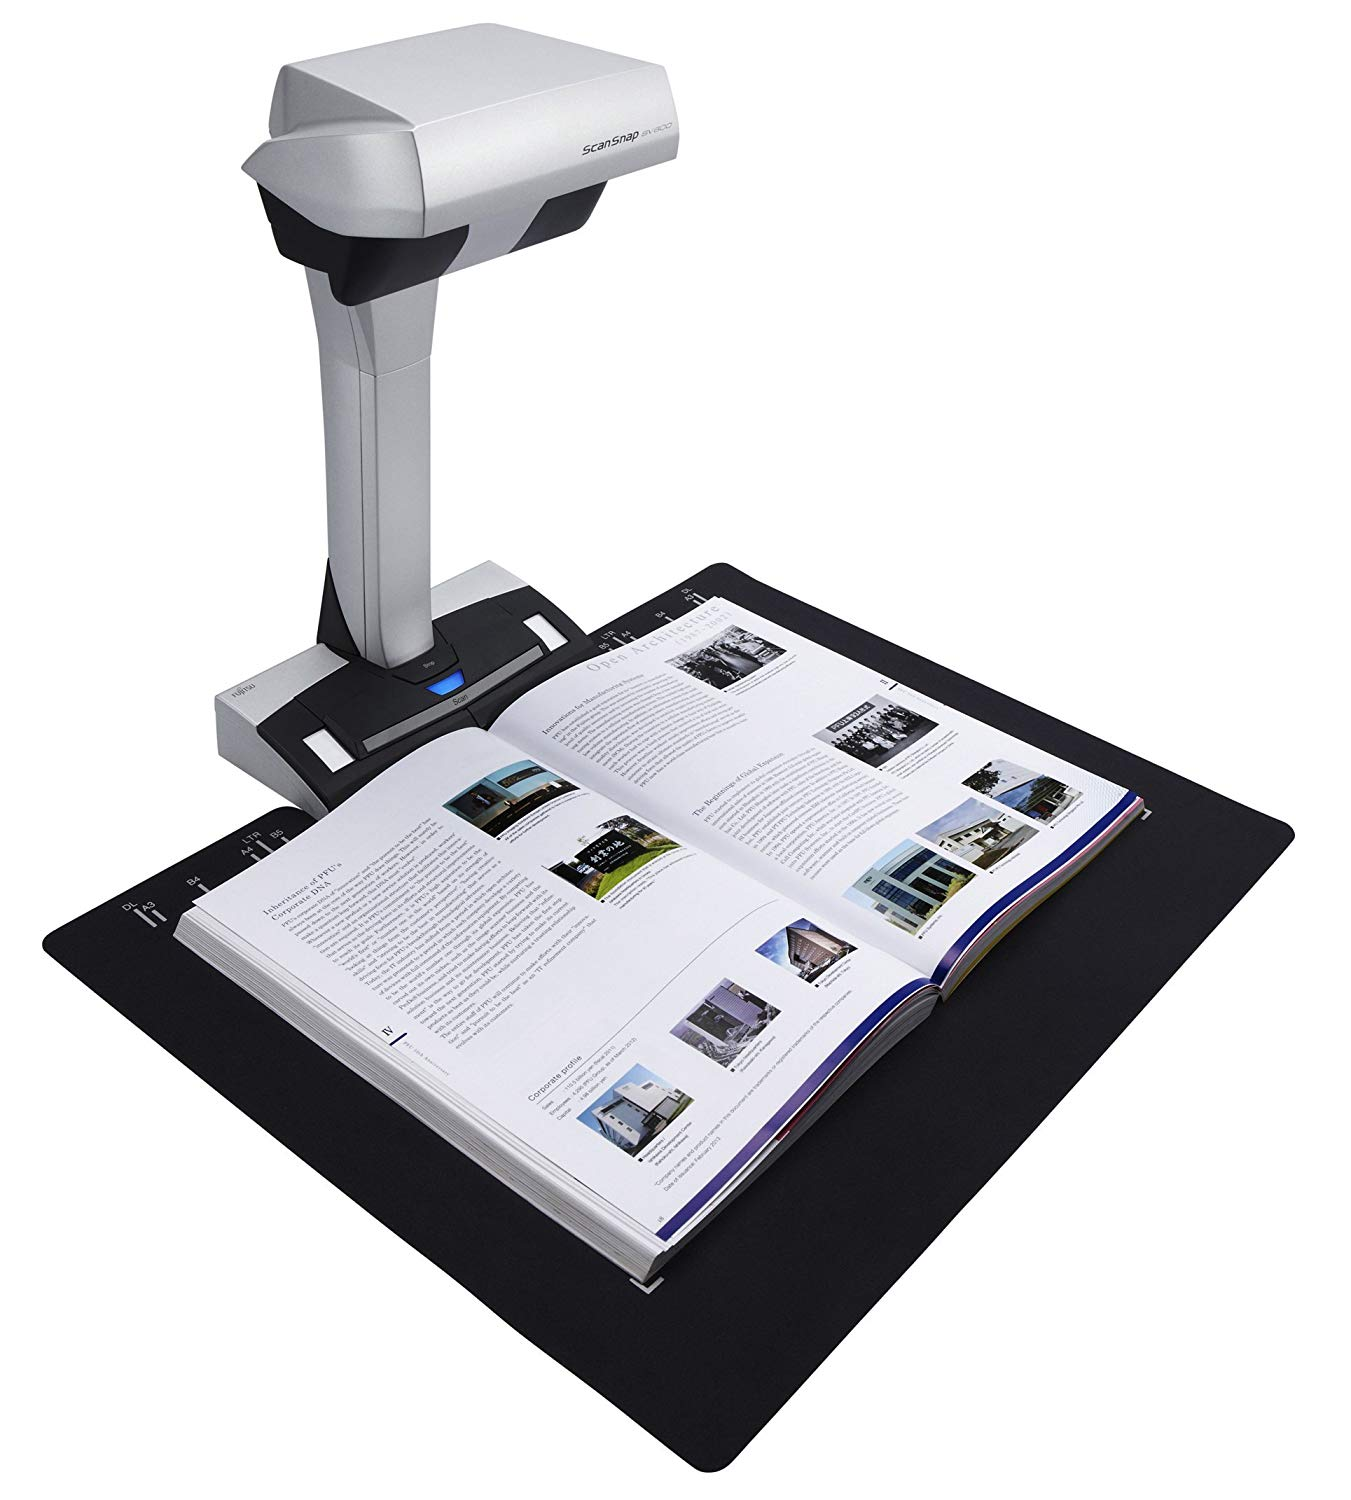
\includegraphics[width=.44\linewidth]{scannerScanSnap}}\hfill
		\subbottom[ET16, de \href{https://www.czur.com/product/et16/}{CZUR}]{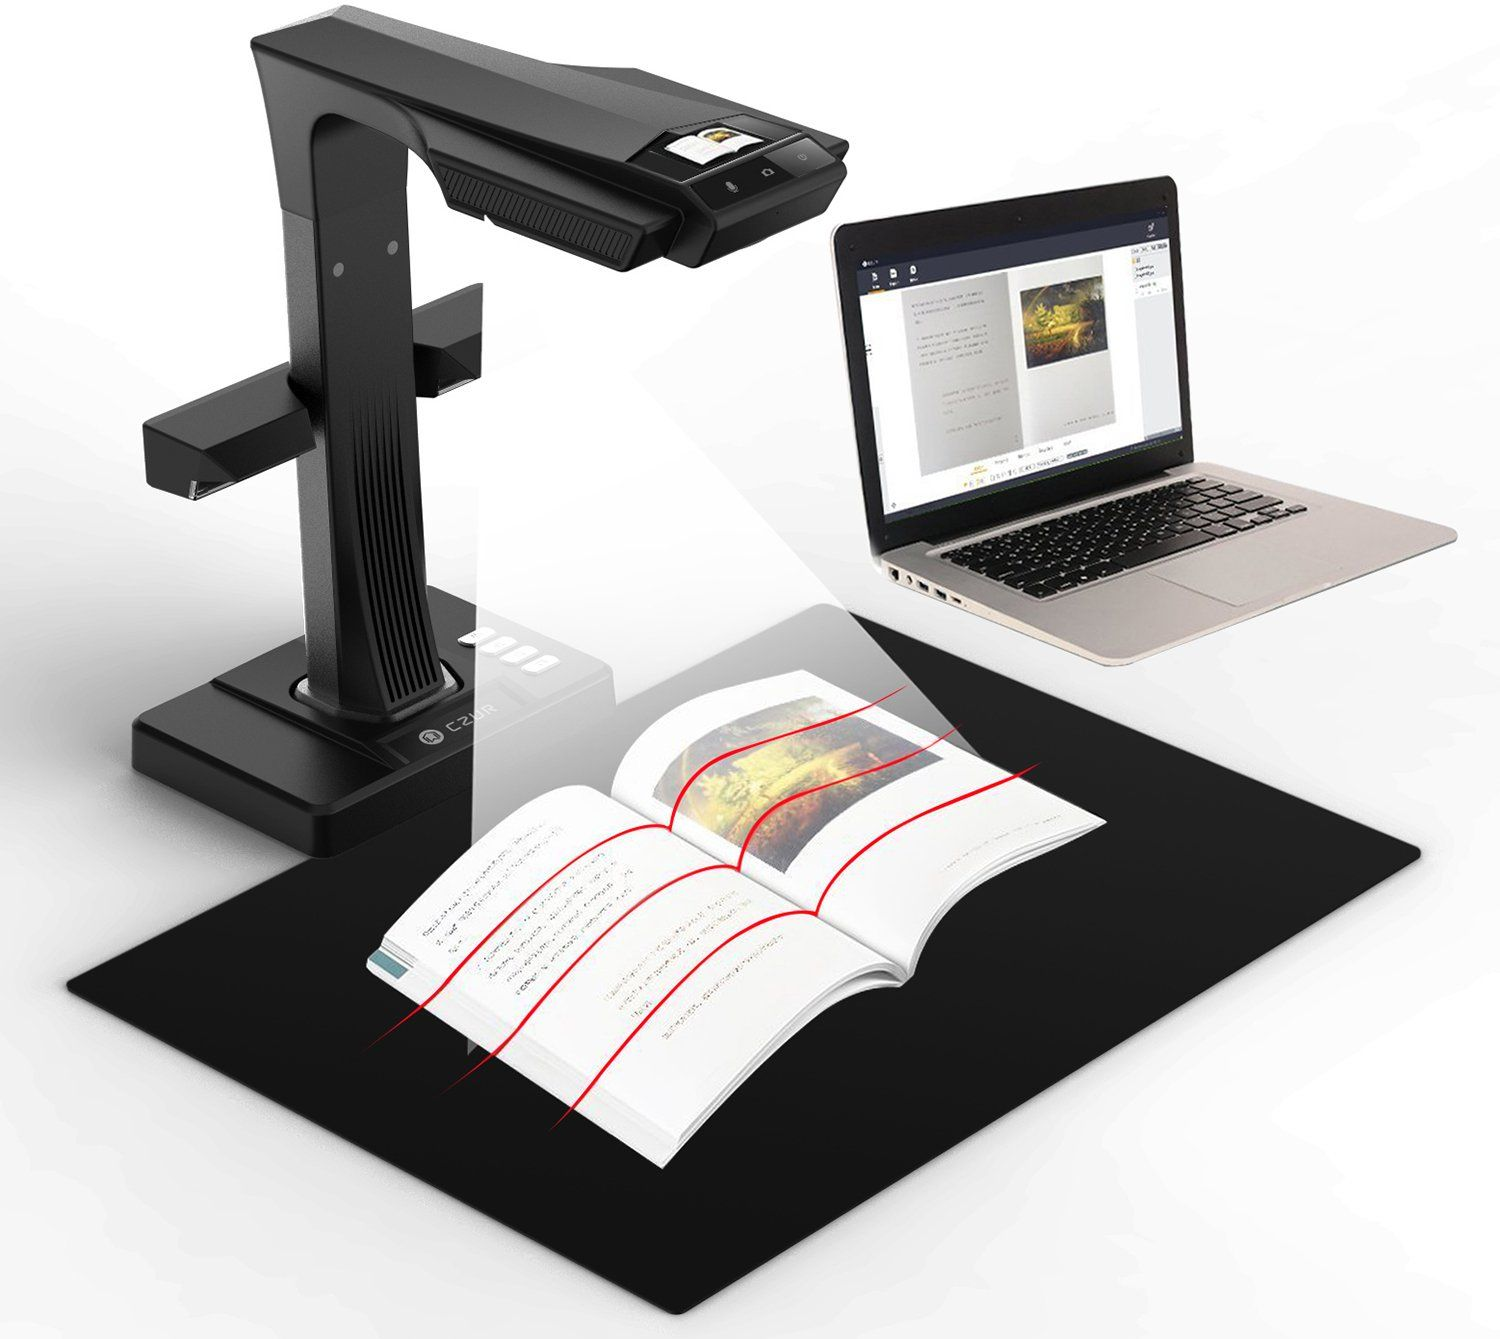
\includegraphics[width=.54\linewidth]{scannerET16}}
		\caption{Dos ejemplos de \emph{book scanners}\label{fig:scannerbookScanners}}
	\end{figure}

	Es de destacar la labor que desde hace años viene realizando la comunidad DIY Book Scanner \cite{DIYBookScanner}, fundada por \href{http://www.danreetz.com}{Daniel Reetz}, para desarrollar soluciones de escaneo accesibles para cualquiera. El sitio y sus foros contienen cantidad de información útil sobre cada etapa tanto de la construcción de un escáner (fig.~\ref{fig:scannerArchivist}) como del posprocesamiento de las imágenes, entre muchos otros temas relacionados.

	\begin{figure}
		\centering
		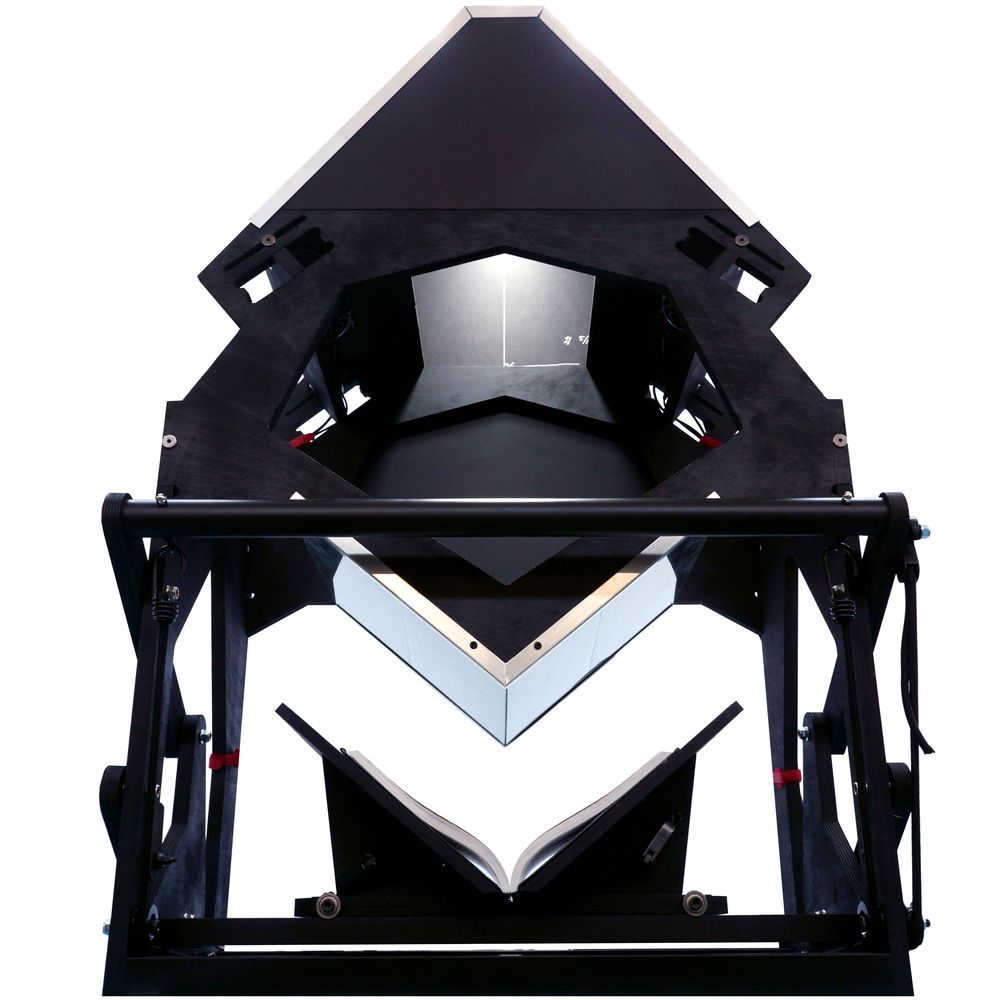
\includegraphics[width=.7\linewidth]{scannerArchivist}
		\caption[The Archivist Book Scanner]{The Archivist Book Scanner. Desarrollado por Daniel Reetz con ayuda de la comunidad \emph{DIY Book Scanner}\label{fig:scannerArchivist}}
	\end{figure}

	Otros proyectos similares y aún en desarrollo son Libreflip \cite{Libreflip}, de \href{https://www.youtube.com/c/ijonberlin}{Ijon Berlin}, y Linear Book Scanner \cite{LinearBookScanner}, de Dany Qumsiyeh.

	\subsubsection{Escáner de cama plana} Estos son los más comunes y económicos. Existen básicamente dos tecnologías: \textsc{cis} y \textsc{ccd}. Hay una cantidad interesante de detalles técnicos, pero básicamente la tecnología \textsc{ccd} es un poco mejor aunque algo más cara. En mi experiencia, cualquiera de los dos funciona suficientemente bien con una gama amplia de materiales mientras se acerque lo suficiente la página al vidrio del escaner \cite{CCDvsCIS}.

	Este tipo de escáneres son los que ofrecen las impresoras multifunción, aunque también se venden por separado.

	Existe una subvariedad en esta categoría, diseñada específicamente para escanear libros. La característica saliente es que el vidrio del escáner llega casi al borde del aparato, lo que permite alcanzar fácilmente el espacio en donde se unen las páginas. Ver ejemplo en la figura~\ref{fig:scannerOpticBook3800}.

	En esta guía utilizo un escáner de cama plana para digitalizar el material. Si se usa otro tipo se deberá hacer algunos ajustes al procedimiento de digitalización.

	\begin{figure}
		\subbottom[Vista general]{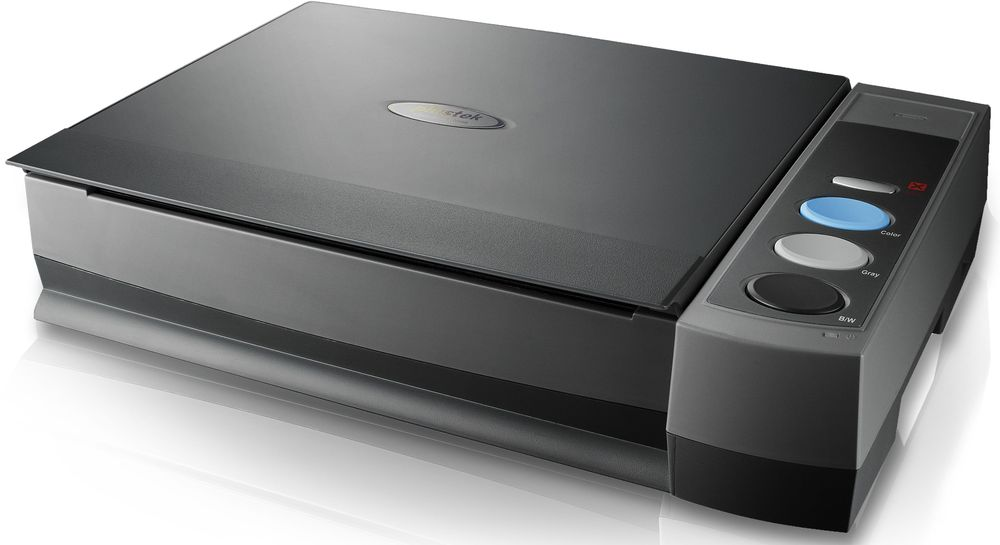
\includegraphics[width=.48\linewidth]{scannerOpticBook3800-1}}\hfill
		\subbottom[Detalle. El vidrio casi alcanza el borde]{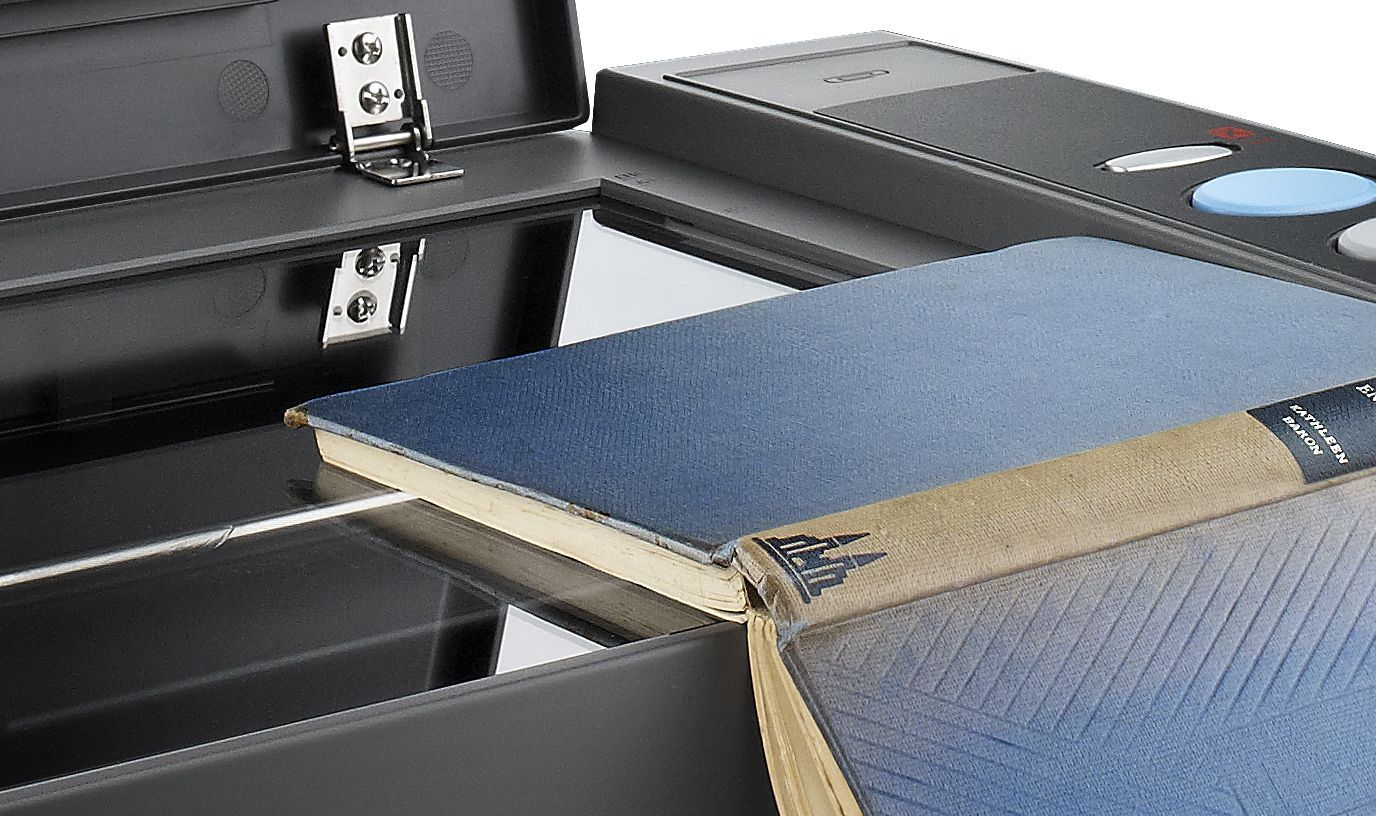
\includegraphics[width=.48\linewidth]{scannerOpticBook3800-2}}
		\caption{OpticBook 3800, de \href{https://plustek.com/es/products/book-scanners/}{Plustek}\label{fig:scannerOpticBook3800}}
	\end{figure}

	\subsubsection{Escáner con \texorpdfstring{\textsc{adf}}{ADF}} \textsc{Adf} significa alimentador automático de documentos (\emph{automatic document feeder}, en inglés). Estos escáneres son muy prácticos, pues toman cada hoja de una pila y la escanean sin necesidad de intervención humana, algunos inclusive por ambas caras. La desventaja es que las hojas a escanear deben estar sueltas. Son muy comunes en las oficinas. Algunos ejemplos en la figura~\ref{fig:scannerADF}.

	\begin{figure}
		\hspace*{\fill}
		\subbottom[Workforce DS-410, de \href{https://www.epson.es/products/scanners}{Epson}]{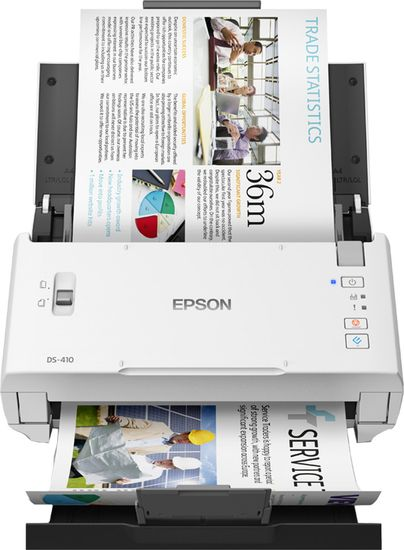
\includegraphics[width=.4\linewidth]{scannerWorkforce}}\hfill
		\subbottom[ScanJet Pro 2500, de \href{https://store.hp.com/SpainStore/Merch/Product.aspx?id=L2747A&opt=B19&sel=SCN}{HP}]{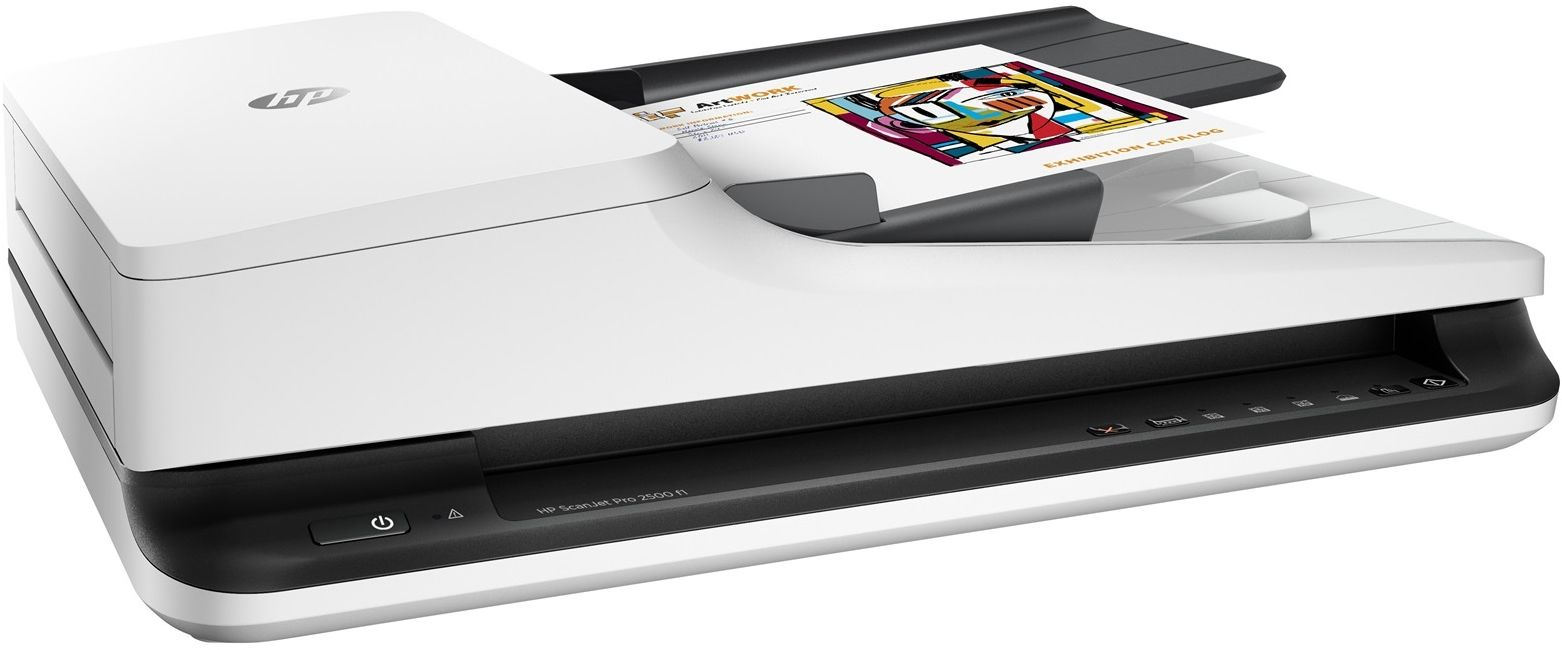
\includegraphics[width=.45\linewidth]{scannerScanJet}}%
		\hspace*{\fill}
		\caption{Escáneres con \textsc{adf}\label{fig:scannerADF}.}
	\end{figure}

	\section{Conclusiones} Los requisitos de software son bastante extensos. La utilidad de cada uno se irá entendiendo a medida que se avance con la guía. Para el hardware existe una variedad importante de opciones de adquisición de imágenes. Dependiendo de cual tengamos a mano será posible usar la guía tal cual o habrá que hacerle modificaciones al flujo de trabajo.

	En el próximo capítulo hablaremos brevemente sobre la estructura que tendrán los archivos de nuestro proyecto.

	\chapter{Estructura del proyecto} Los archivos de nuestro proyecto estarán estructurados en un árbol de carpetas como el de la figura~\ref{fig:projectStructure}. Habrá una carpeta base llamada \typesetFolder{Project}, dentro de la que iremos creando las siguientes. Esta carpeta base puede estar en cualquier lugar de nuestro \textsc{pc}. Normalmente la coloco en la raíz del disco \typesetFolder{C:}, pero los scripts que utilizaremos deberían funcionar sin importar donde esté ubicada, mientras se respete la estructura del árbol.\footnote{Hay excepciones que se mencionan específicamente.}

	\begin{figure}
		\hspace*{\fill}
		\begin{forest}
			for tree={font=\sffamily, grow'=0,
				folder indent=.9em, folder icons,
				edge=densely dotted}
			[Project
			[ABBY]
			[Batches]
			[djv]
			[SCAN]
			]
		\end{forest}\hfill
		\begin{forest}
			for tree={font=\sffamily, grow'=0,
				folder indent=.9em, folder icons,
				edge=densely dotted}
			[SCAN
			[foreground]
			[background]
			[out]
			]
		\end{forest}%
		\hspace*{\fill}
		\caption{Árbol de directorios del proyecto\label{fig:projectStructure}}
	\end{figure}

	En \typesetFolder{SCAN} irán nuestras exploraciones hechas con el escáner. Dentro de esa carpeta tendremos \typesetFolder{out}, donde \scantailor guardará las imágenes procesadas. A su vez, podrían estar \typesetFolder{foreground} y \typesetFolder{background}, donde se guardarán independientemente el texto y las imágenes.

	En \typesetFolder{Batches} guardaremos los scripts y algunos archivos asociados a ellos.

	En la carpeta \typesetFolder{ABBY} irá nuestro proyecto de \abby. Dentro de esa carpeta el programa creará muchas otras, con la estructura que se describe en el apéndice~\ref{sec:abbyProjectStructure}.

	En \typesetFolder{djv} guardaremos varios documentos \pdf y \djvu, que corresponderán a las distintas etapas de procesamiento.

% ------------------------------------------------------------------------------
% ---------------------------------  PART II   ---------------------------------
% ------------------------------------------------------------------------------
	\part{Procedimiento}

	\chapter{Introducción\label{sec:procedure}} En esta parte se explica cada paso del proceso hasta la producción de los archivos digitales.

	Como ejemplo vamos a utilizar un libro de instrumentación y medidas de B.~A. Gregory \cite{GregorySpringer}.\footnote{Para más información, ver el apéndice~\ref{sec:aboutGregory}.}

	Comenzaremos explicando los trabajos de escaneo del material original: preparación del escáner, preparación del material, configuración del software de escaneo, proceso de escaneo y posibles complicaciones.

	Luego pasaremos al procesamiento de las imágenes adquiridas, para el que utilizaremos fuertemente el software \scantailor.

	El siguiente paso será reconocer el texto con \abby. Para ello deberemos configurarlo adecuadamente y habrá una cantidad de obstáculos que tendremos que evitar.

	Por último crearemos los documentos finales en formato \pdf y/o \djvu. Deberemos agrupar las imágenes en estos archivos y agregarles el texto reconocido, las imágenes, los marcadores, etiquetas de páginas y metadatos.

	Sin más dilaciones: ¡comencemos!.

	\chapter{Escaneo\label{sec:scanning}} La regla número uno para obtener un buen resultado es comenzar con buen material de base. En el caso que nos ocupa necesitaremos imágenes de buena calidad, es decir: de adecuada resolución, almacenadas en el formato adecuado, usando el algoritmo adecuado, sin artefactos, etc. En esta sección veremos algunas recomendaciones para conseguirlas. Recomiendo antes visitar \cite{ScanTips}.

	\section{Estado del aparato\label{sec:scanningState}} Lo primero que debemos hacer es revisar el escáner que vayamos a usar. Para ello puede ser útil tener a mano una linterna. El vidrio debe estar limpio, libre de grasa, vellos, polvo y cualquier otro tipo de suciedad. Lo mismo la parte interna de la cubierta del escáner, pues aunque muchas veces no se use podría dejar caer suciedad sobre el vidrio. Si no lo están, deben primero limpiarse según las especificaciones del fabricante. En caso de que no existan, un paño de microfibra o papel absorbente apenas humedecido con agua (o mejor aun alcohol isopropílico) podría funcionar. Si el vidrio se encuentra rayado conviene hacer alguna exploración de prueba para ver si la afecta apreciablemente.\footnote{Sobre una página completamente blanca se aprecia bien.} De ser así deberemos evitar esa zona del escáner y, en caso de no poder hacerlo, procurar otro aparato.

	Además, deben haberse instalado correctamente los drivers y el software de digitalización. En caso de tener problemas con esto, lo mejor será consultar en la web del fabricante o algún foro de soporte en internet.

	\section{Preparación del material\label{sec:scanningPreparingMaterial}} ¡¿Hay que preparar el libro?! Bueno, eso dependerá de varias cosas.

	Lo primero que debemos preguntarnos es que valor (sentimental o material) tiene lo que vamos a escanear, y cuanto de ese valor estamos dispuestos a sacrificar o a poner en riesgo.

	Si estamos hablando de un libro barato o al que no nos sentimos apegados, la opción más eficiente es cortarle el lomo en una guillotina\footnote{O cortar sus páginas de una, para los que tengan paciencia.} y colocarlo en un escáner \adf. Si no tenemos ese tipo de escáner, de todas formas es más fácil colocar las hojas sueltas en uno de cama plana y conseguir digitalizaciones de muy buena calidad. Luego de esto se pueden tirar las hojas o, si vale la pena, enviarlas a reencuadernar.

	Si el material no puede ser destruido, debemos preguntarnos si aún así no puede ser abusado. Es decir, ¿podemos permitirnos abrirlo 180\textdegree\ y apretarlo con fuerza contra el vidrio del escáner? He escaneado muchos libros de esta manera y salvo algunas excepciones nunca han perdido páginas ni quedado con daños permanentes, pero esa evaluación la debe hacer cada persona. %your mileage may vary
	Aún si estamos dispuestos, podría ocurrir que no logremos buenos resultados en la parte donde se unen las hojas (fig.~\ref{fig:epsonScan}). Para estar seguros podemos hacer algunas previsualizaciones de prueba.

	Si seguimos sin encontrar la solución, debemos considerar adquirir otro tipo de escáner. O tal vez otro ejemplar de la obra que tenga menos valor y permita estos abusos.

	Los productos que fabrica para esto Plustek funcionan bastante mejor, pero igual se debe hacer algo de presión sobre el lomo para que toda la imagen sea clara, sobre todo en volúmenes muy gruesos.

	Luego están los \emph{book scanners} comerciales, pero por estar pensados para materiales que no pueden ser abusados, dependen mucho del software que traen para corregir las aberraciones ópticas que tiene la imagen, producto de que la página nunca se encuentra plana respecto a las cámaras.

	Un punto intermedio es el Archivist o similares, que abren los libros solo unos 135\textdegree\ y suavemente presionan una cuña de vidrio para aplanar las páginas.

	No se desanime si su caso no está cubierto en estas líneas. Piense, experimente, pregunte. Esta guía no no lo cubre todo y la solución que necesita para su proyecto puede estar a la vuelta de la esquina.

	\subsection{¿Qué partes escanear?\label{sec:scanningWhatToScan}} Antes de continuar hay un aspecto importante que no quisiera dejar de resaltar. En general, pero sobre todo si se trata de un libro publicado, escaneémoslo de cubierta delantera a cubierta trasera, sin dejar fuera absolutamente nada: ni páginas en blanco (llamadas de respeto o de cortesía), ni páginas de copyright, ni índices, ni apéndices, ni lomo\... Todo tiene su razón para estar allí y hace a la calidad de la publicación (y, por ende, de la digitalización), por lo que no hay motivo para dejar fuera nada.

	\subsection{Fotos\label{sec:scanningPhotos}} A lo largo de la guía usaremos el vocablo «fotos» para referirnos a las ilustraciones o fotografías, a color o en escala de grises, impresas en el material que estamos digitalizando. Esto para distinguirlas de otras ilustraciones o diagramas simples que no requieran del tratamiento especial que describe la sección «Picture zones» (\ref{sec:SToutputPictureZones}).

	\section{Configuración del software\label{sec:scanningSoftware}} El paso siguiente es configurar el software de escaneo. Generalmente, este viene pensado para que se pueda usar sin pensar demasiado y que aún así puedan obtenerse buenos resultados. Por ello ya se incluyen cantidad de herramientas de posprocesado (mejora de la nitidez, desinclinación, balance de blancos, separación de varias imágenes, entre muchas otras). Debemos desactivarlas todas. Tengamos en cuenta que de ser necesarias algunas de estas correcciones podremos realizarlas más adelante y con mucho más control utilizando programas adicionales.

	Abrimos el \irfanview y elegimos \menu{File > Acquire/Batch Scanning\...} obteniendo el cuadro de diálogo de la figura~\ref{fig:scanningIrfanViewBatch}. Debemos seleccionar \menu{\typesetDotCircle{Multiple images (Batch mode)}}, luego en \menu{Output file name > SCAN\_}, en \menu{Number of digits > 3}\footnote{o \menu{4} si nuestro proyecto contiene 1000 páginas o más.} y en \menu{Destination directory > C:\textbackslash Project\textbackslash SCAN}. Es conveniente activar \menu{\typesetCheckbox{Skip existing files}} y \menu{\typesetCheckbox{Remember last scan counter}}.

	\subsection{Formatos\label{sec:scanningSoftwareFormats}} En este punto debemos elegir el formato de archivo para guardar las exploraciones. \irfanview ofrece muchos, pero dos que funcionan bien son \tiff y \png.

	Para \tiff elegimos la opción \menu{TIF - Tagged Image File Format} del menú \menu{Save as} y presionamos \keys{Options}. Allí aparece el cuadro de la figura~\ref{fig:scanningIrfanViewBatchTIF}, donde se debe seleccionar el tipo de compresión. Sin entrar en más detalles, elegimos \menu{\typesetDotCircle{LZW}}, pues no tiene pérdidas (\emph{lossless}) y ofrece un grado razonable de compresión. Otras alternativas sin pérdidas son \menu{\typesetCircle{ZIP}}, que alguna vez me dio problemas con el \scantailor y \menu{\typesetCircle{Packbits}}, que no he probado. Por ninguna razón elegir \menu{\typesetCircle{JPEG}}, pues introduce pérdidas (\emph{lossy}) o \menu{\typesetCircle{None}} (sin compresión) porque genera archivos enormes.\footnote{Nuestro proceso contendrá muchos archivos temporales de gran tamaño que al final terminarán en un documento de tamaño razonable. Estos archivos temporales podrán ser borrados al terminar, pero si de todas formas pudiéramos ahorrar algo de espacio durante el proceso lo haremos.}

	La alternativa a \tiff es \png. El algoritmo de compresión de \png es siempre sin pérdidas. Elegimos \menu{PNG - Portable Network Graphics} y presionando en  \keys{Options} vemos el cuadro de la figura~\ref{fig:scanningIrfanViewBatchPNG}, donde ingresamos \menu{Compression level > 9}. Activando la casilla \menu{\typesetBox{Use PNGOut PlugIn}} podemos mejorar ligeramente la compresión pero a un costo computacional muy alto, que no vale la pena, por lo que la dejamos desactivada.

	\begin{figure}
		\centering
		\subbottom[Menú \menu{Acquire/Batch Scanning\...}\label{fig:scanningIrfanViewBatch}]{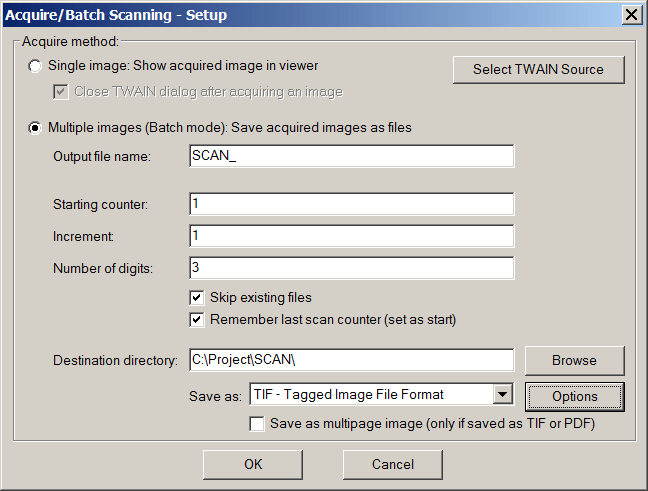
\includegraphics[width=\linewidth]{scanningIrfanViewBatch}}\\
		\subbottom[Opciones del formato \menu{TIF}\label{fig:scanningIrfanViewBatchTIF}]{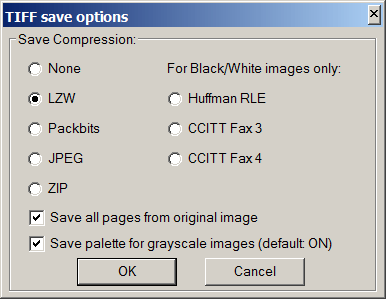
\includegraphics[width=.49\linewidth]{scanningIrfanViewBatchTIF}}\hfill
		\subbottom[Opciones del formato \menu{PNG}\label{fig:scanningIrfanViewBatchPNG}]{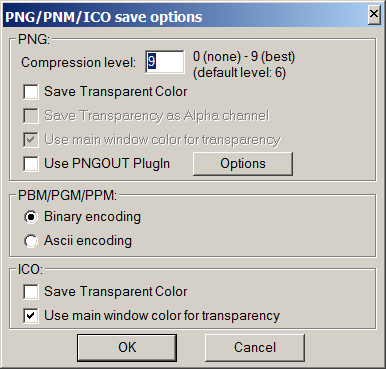
\includegraphics[width=.49\linewidth]{scanningIrfanViewBatchPNG}}
		\caption{Ajustes de escaneo del \irfanview\label{fig:scanningIrfanView}}
	\end{figure}

	Luego de elegir las opciones presionamos \keys{OK} y si el escáner está bien configurado debería iniciarse el software correspondiente. Como ejemplo usaremos el programa EPSON~Scan (v5.7.9.3). En la figura~\ref{fig:epsonScan} se muestra la ventana principal. Podemos ver que se ofrecen varios \menu{Modos}: \menu{Automático}, \menu{Fácil}, \menu{Oficina} y \menu{Profesional}. Por supuesto elegimos \menu{Profesional}.

	Comenzamos por colocar una página representativa\footnote{Elegí una donde haya tanto texto como fotografías.} del material a escanear y luego presionamos \keys{Previsualización}, lo que nos dará un resultado como el de la fig.~\ref{fig:epsonScan}. En caso de que la región a escanear no ocupe toda la superficie del escáner, conviene seleccionarla dibujando un rectángulo en la pestaña de \menu{Previsualización}, de esta forma se agilizan un poco los tiempos de escaneo. \label{pag:scanningRegionSelection} Para que esta opción funcione bien cada página a escanear debe ser colocada dentro de la misma zona seleccionada. De lo contrario podría quedar contenido fuera.

	\begin{figure}
		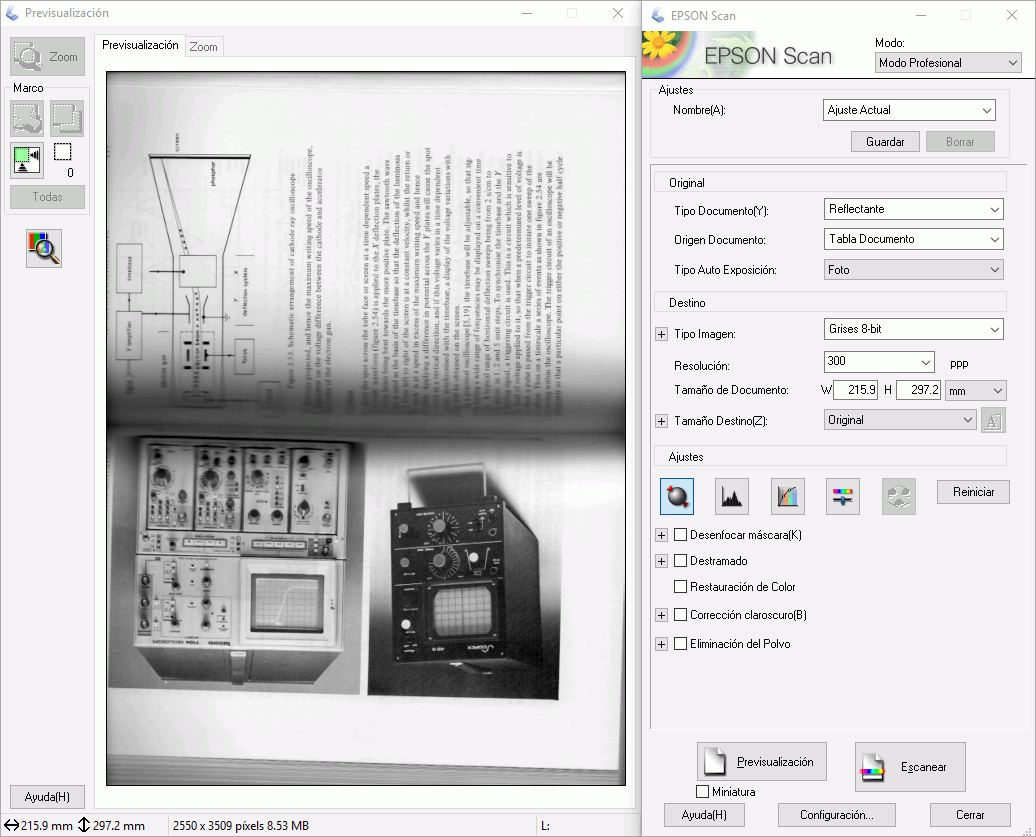
\includegraphics[width=\linewidth]{epsonScan}
		\caption[Ventana principal del EPSON Scan]{Ventana principal del EPSON Scan. Se previsualizaron dos páginas representativas\label{fig:epsonScan}}
	\end{figure}

	En nuestro caso las opciones \menu{Tipo Documento(Y)} y \menu{Origen Documento} no se pueden modificar. \menu{Tipo Auto Exposición} se explica más abajo.

	En \menu{Tipo de imagen} elegimos \menu{Color 24-bit} o \menu{Grises 8-bit}, dependiendo de si la página es a color o no. Se ofrecen también \menu{Suavizado de Color} y \menu{Ninguno}. Según la documentación de Epson la primera es para «gráficos a color, como un diagrama o un gráfico». La segunda no tiene un nombre muy explícito pero significa bitonal. Es decir, blanco o negro. Esta opción puede ser tentadora porque generalmente produce un tamaño de archivo más pequeño. Sin embargo, se pierde muchísima información de la página (fig.~\ref{fig:epsonScanBitonal}). Nuestro resultado final será en general bitonal, pero luego de todo el procesamiento tendremos imágenes de excelente calidad e ínfimo tamaño. Por todo esto, no debe usarse ninguna de estas dos opciones u otras similares que puedan ofrecer las aplicaciones de los distintos fabricantes.

	\begin{figure}
		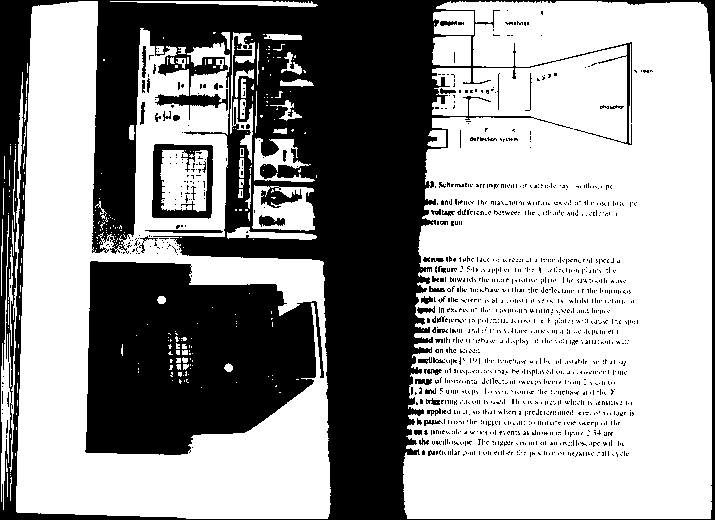
\includegraphics[angle=-90, width=\linewidth]{epsonScanBitonal}
		\caption[Páginas representativas escaneadas en bitonal]{Páginas representativas escaneadas seleccionando la opción \menu{Tipo de imagen > Ninguno} (bitonal). Nótese que las fotografías están arruinadas y que el texto se vuelve ilegible\label{fig:epsonScanBitonal}}
	\end{figure}

	La \menu{Resolución} es uno de los parámetros más importantes. La óptima es de 300\,dpi (ppi o ppp) y es la que usaremos en esta guía. Así se obtiene un buen resultado final y no se hace eterno el tiempo que se está presionando el libro contra el escáner. 600\,dpi sería aún mejor, pero en los escáneres comunes cada exploración toma mucho más tiempo. Valdrá la pena solo para páginas con un nivel muy alto de detalles. Si bien la elección final dependerá de cada caso, escanear a menos de 300\,dpi será siempre un desperdicio, por la cantidad de detalles que se perderán.

	\menu{Tamaño de Documento} se ajustará a la región que hayamos seleccionado (si lo hicimos) y \menu{Tamaño de Destino(Z)} debe decir \menu{Original}.

	Como se muestra, recomiendo la desactivación de todas las casillas: \menu{\typesetBox{Desenfocar máscara(K)}}, \menu{\typesetBox{Destramado}}, \menu{\typesetBox{Restauración de Color}},\\\menu{\typesetBox{Corrección claroscuro(B)}}, \menu{\typesetBox{Eliminación del Polvo}} y cualquier otra que ofrezca el software que estemos usando, por las razones aducidas al principio de esta sección.

	En la parte de \menu{Ajustes} hay una serie de íconos que representan distintos tipos de ajustes que se pueden aplicar. Al presionar \keys{Previsualización} o cambiar el área seleccionada se activa automáticamente el primero, que es el de \menu{Autoexposición}. Este ajusta a todos los demás en función del contenido previsualizado (o el área seleccionada) y la opción \menu{Tipo Auto Exposición} elegida.

	A veces no utilizo la opción de \menu{Autoexposición} sino que presiono \keys{Reiniciar} y dejo todos los valores por defecto. Otra alternativa, que es la que empleé en esta guía, es realizar un autoajuste con una página representativa y usarlo para todas las demás. En caso de dudas lo mejor es experimentar.

	\section{A escanear} Una vez preparado todo, podemos comenzar a escanear. Para ello presionamos \keys{Escanear}. El equipo hará una exploración y el \irfanview irá mostrando y guardando las imágenes de acuerdo a las opciones seleccionadas. Lo hará usando el nombre base (\menu{Output file name}) y aumentando la numeración. Es importante que el orden creciente de las páginas del libro corresponda con el orden creciente de los números de los archivos, para que no haya confusión a la hora de compaginar todo. Además, algunos scripts y aplicaciones que usaremos luego dependerán de que esta numeración sea consistente a lo largo de todo el proyecto para funcionar correctamente.

	Si el libro es suficientemente pequeño podremos ir escaneando de a dos páginas a la vez, de lo contrario será de a una. Luego de un rato trabajando veremos que el proceso transcurre prácticamente sin pensar. Llegado ese punto yo aprovecho para paralelamente mirar televisión, escuchar música o meditar sobre lo humano y lo divino.

	Conviene que las páginas estén rectas respecto a los bordes de la superficie de exploración, pero sin necesidad de perfección. Durante el procesamiento podremos corregir algunas desviaciones.

	Es buen momento para poner sobre la mesa de cuanto tiempo estamos hablando. En el caso de este libro usé un escáner OpticBook~3800 configurado en 300\,dpi y grises~8-bit. Escaneé las primeras 200 páginas de un tirón (una página por exploración y habiendo seleccionado la región en el área de \menu{Previsualización}), lo que me llevó unos 40~minutos. Estamos hablando entonces de un promedio de 5\,pág/min. El libro tiene unas 450 páginas por lo que en total debería llevar al menos 90 minutos. Por supuesto que luego hay que revisar y reescanear las que no hayan quedado bien.

	Al finalizar deberíamos contar con tantos archivos como páginas tiene el libro salvo que hayamos adquirido de a dos, en cuyo caso serán aproximadamente la mitad de archivos (tapa, contratapa y lomo se adquieren de una). Conviene hacer una inspección visual de cada imagen para ver si alguna no quedó del todo bien y necesita escanearse de nuevo. A continuación veremos algunos de los problemas con los que nos podríamos enfrentar y como remediarlos.

	\subsection{Páginas faltantes} Siempre habrá que ir chequeando que no se nos pase por alto alguna página, y si ocurre remediarlo acomodando los nombres de los archivos, de forma de que aquel que haya sido salteado quede intercalado correctamente. Para esto puede ser útil el \textsc{Advanced Renamer}.

	En el ejemplo que estamos trabajando, la página 10 del libro corresponde al archivo \typesetFile{SCAN\_022.tif}, es decir que hay un desfasaje de 12 páginas. Un forma rápida de chequear que no falte ninguna es ver que el archivo \typesetFile{SCAN\_112.tif} corresponda con la página 100, el \typesetFile{SCAN\_212.tif} con la 200, y así\...

	De esta forma descubrí que me faltó escanear la página 99 (+ 12 = archivo 111). Usando \textsc{Advanced Renamer} desplacé los nombres de los archivos un lugar: \typesetFile{SCAN\_112.tif} \faLongArrowAltRight\ \typesetFile{SCAN\_113.tif}, \typesetFile{SCAN\_111.tif} \faLongArrowAltRight\ \typesetFile{SCAN\_112.tif}, \...\footnote{Por si no quedó claro, el programa permite renombrar fácil e instantáneamente todos los archivos de la manera que el usuario elija. \emph{No} se hizo uno por uno.} De esta forma quedó el nombre \typesetFile{SCAN\_111.tif} libre para la página que faltaba. Entonces la escaneé y le puse ese nombre.

	En cualquier momento podemos reiniciar el proceso de escaneo a partir del número de página que elijamos.

	\subsection{Curvatura y contenido fuera del área} Si no presionamos bien el lomo sobre el vidrio del escáner, obtendremos imágenes con sombras y distorsiones cerca del margen interior, debido a que el papel no está plano respecto al sensor. Ver un ejemplo en la figura~\ref{fig:scanningIrfanView}.

	\begin{figure}
		\subbottom[Curvatura y sombra]{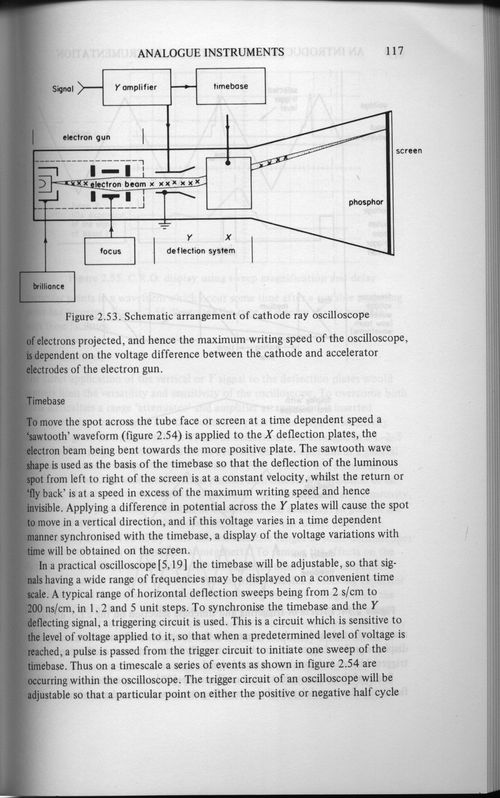
\includegraphics[width=.49\linewidth]{distortionCurveShadow}}\hfill
		\subbottom[Contenido fuera del área]{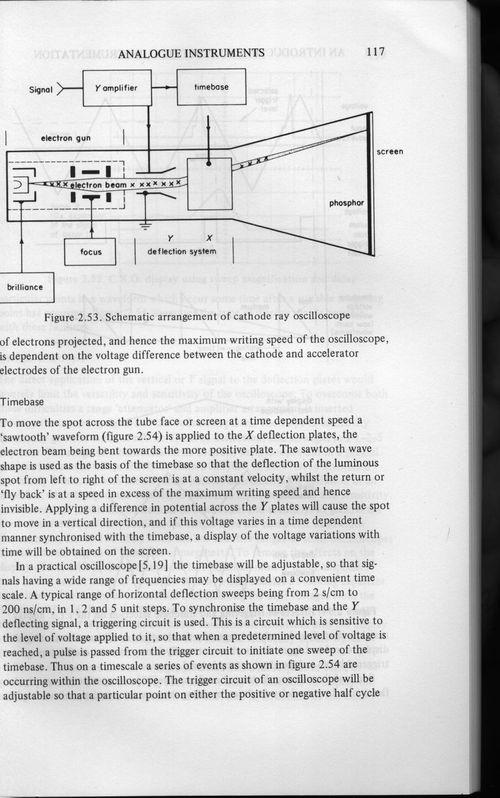
\includegraphics[width=.49\linewidth]{distortionCut}}
		\caption{Distorsiones y sombras sobre el margen interior\label{fig:distortion1}}
	\end{figure}

	Si la sombra es pronunciada podría dar problemas durante la binarización. A su vez, si los contenidos están deformados no preservaremos exactamente el material original y probablemente dificultemos el \ocr.

	Por otra parte, si no colocamos correctamente el material, podría ocurrir que parte del contenido de interés quedase fuera del área de exploración (fig.~\ref{fig:distortion1}).

	En todos estos casos, la mejor solución será escanear de nuevo estas páginas.\footnote{Deberemos escanear de nuevo solamente si estas distorsiones afectan al texto o las imágenes. Si apenas caen dentro del blanco de página podremos ignorarlas.}

	\subsection{Distorsiones trapezoidal y por movimiento} La distorsión trapezoidal, llamada en inglés \emph{keystone effect}, es prácticamente inexistente en los escáneres de cama plana, pero se trata de la número uno en los basados en cámaras fotográficas. Es una deformación que se produce por no estar el material perfectamente perpendicular al sensor de la cámara. El ejemplo de la figura~\ref{fig:keystone} fue tomado con la cámara de un teléfono celular. Si no puede corregirse ajustando el hardware, existen algunas soluciones de software que funcionan si la distorsión es moderada. En particular, \scantailor tiene la pestaña \menu{Dewarping} en el paso 6, pero aún se considera experimental y no tengo experiencia con ella.

	También podría ocurrir que el material se moviera mientras el sensor del escáner avanza, provocando compresión o estiramiento de las líneas si es en la misma dirección del avance, o deformación lateral si es en la dirección perpendicular (fig.~\ref{fig:movimiento}). En este caso también deberá escanearse de nuevo.

	\begin{figure}
		\subbottom[Trapezoidal. Se dibujó el trapecio\label{fig:keystone}]{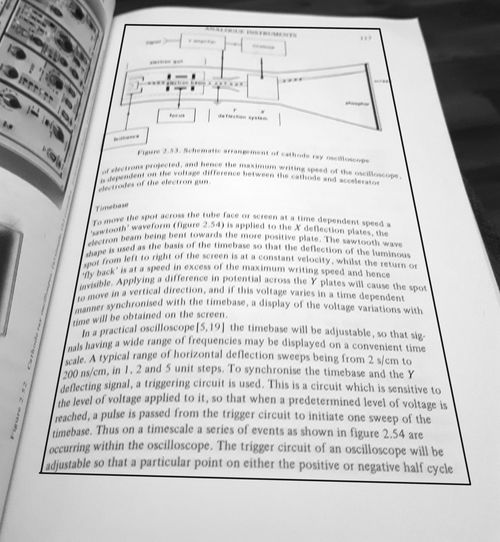
\includegraphics[width=.59\linewidth]{distortionKeystone}}
		\subbottom[Movimiento\label{fig:movimiento}]{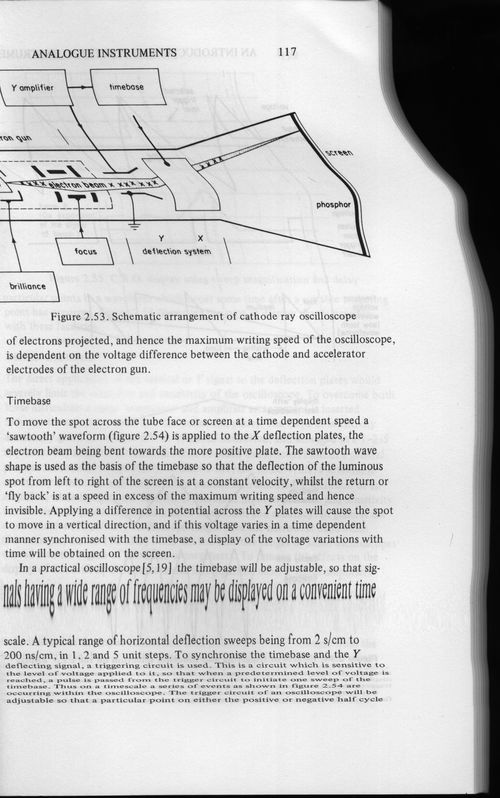
\includegraphics[width=.4\linewidth]{distortionMovement}}\hfill
		\caption{Distorsiones trapezoidal y por movimiento\label{fig:distortion2}}
	\end{figure}

	\subsection{Transparencia de páginas} Dependiendo del tipo de papel y la tinta que se hayan usado puede ocurrir que sobre cada página se transparenten los contenidos de las contiguas. Normalmente este es un inconveniente que desaparece durante la binarización, pero en el caso de las fotografías o imágenes complejas es más persistente y en algunos casos es fácil de tratar.

	Ampliando en la figura~\ref{fig:distortion1} vemos que es posible distinguir el texto y los diagramas de las páginas contiguas. En la figura~\ref{fig:transparencyText} se muestra con más detalle.

	Para disminuir el efecto de las transparencias sobre las fotografías (fig.~\ref{fig:transparencyPhoto}) puede colocarse un papel de color negro\footnote{Usé una hoja impresa en negro por las dos caras. Según el caso, podría funcionar mejor otro color.} entre la página que se va a escanear y la siguiente (o anterior; fig.~\ref{fig:transparencyPaper}). Es decir que tendríamos el vidrio del escáner, luego la página que estamos escaneando, luego el papel negro y finalmente las demás hojas. El resultado se ve en la figura~\ref{fig:transparencyPhotoFix}.

	\begin{figure}
		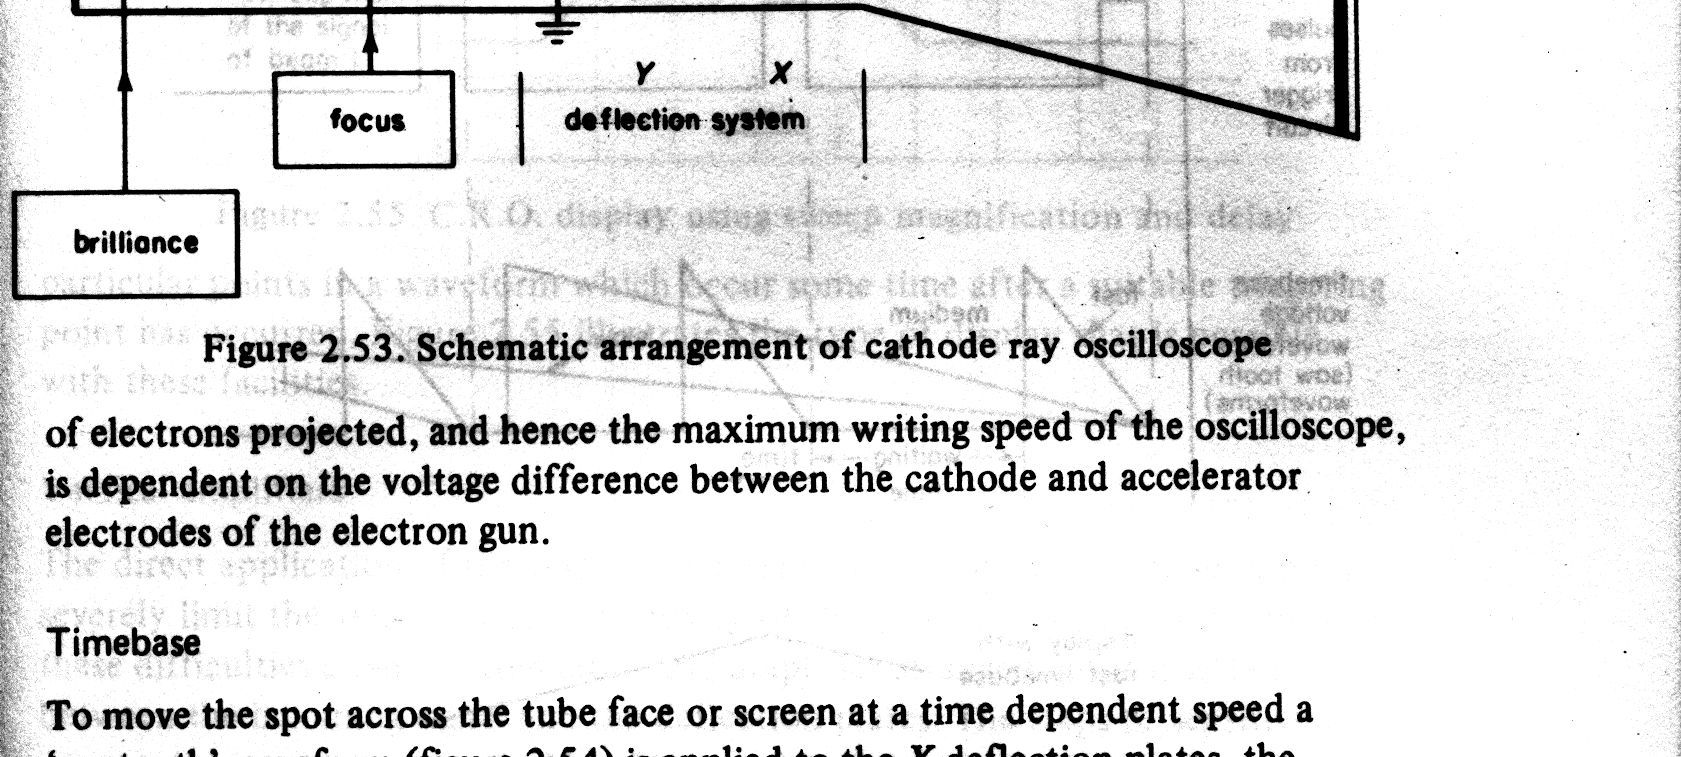
\includegraphics[width=\linewidth]{transparencyText}
		\caption[Transparencia sobre texto y diagramas]{Transparencia sobre texto y diagramas. (Se ha acentuado para que se distinga con claridad.)\label{fig:transparencyText}}
	\end{figure}

	\begin{figure}
		\vspace{-1.11\onelineskip}
		\subbottom[Transparencias sobre fotografías\label{fig:transparencyPhoto}]{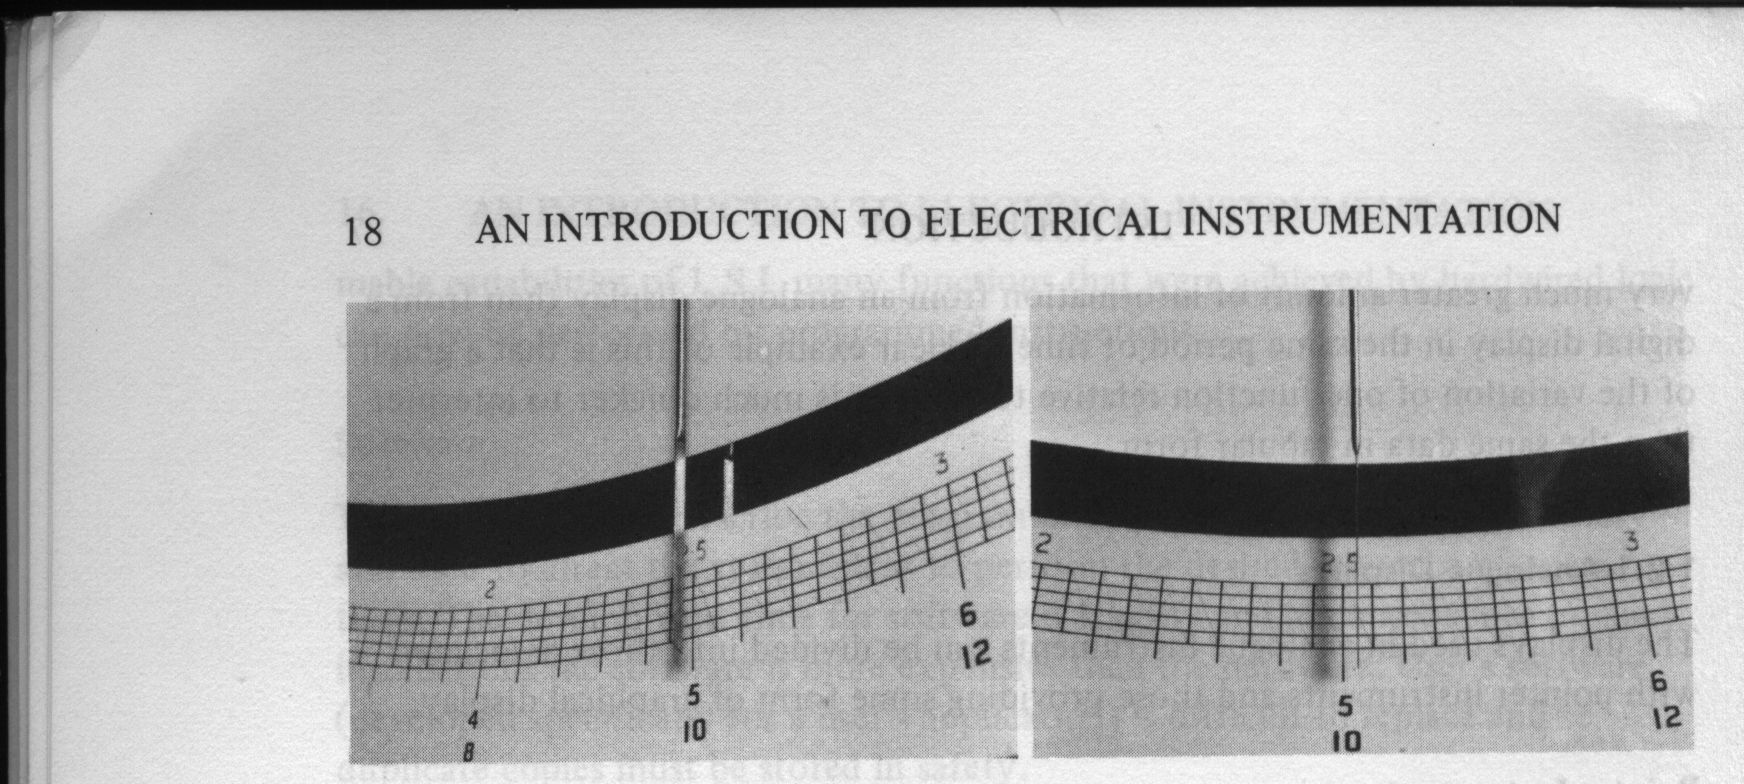
\includegraphics[width=\linewidth]{transparencyPhoto}}
		\subbottom[Mitigado el efecto usando un papel negro por debajo\label{fig:transparencyPhotoFix}]{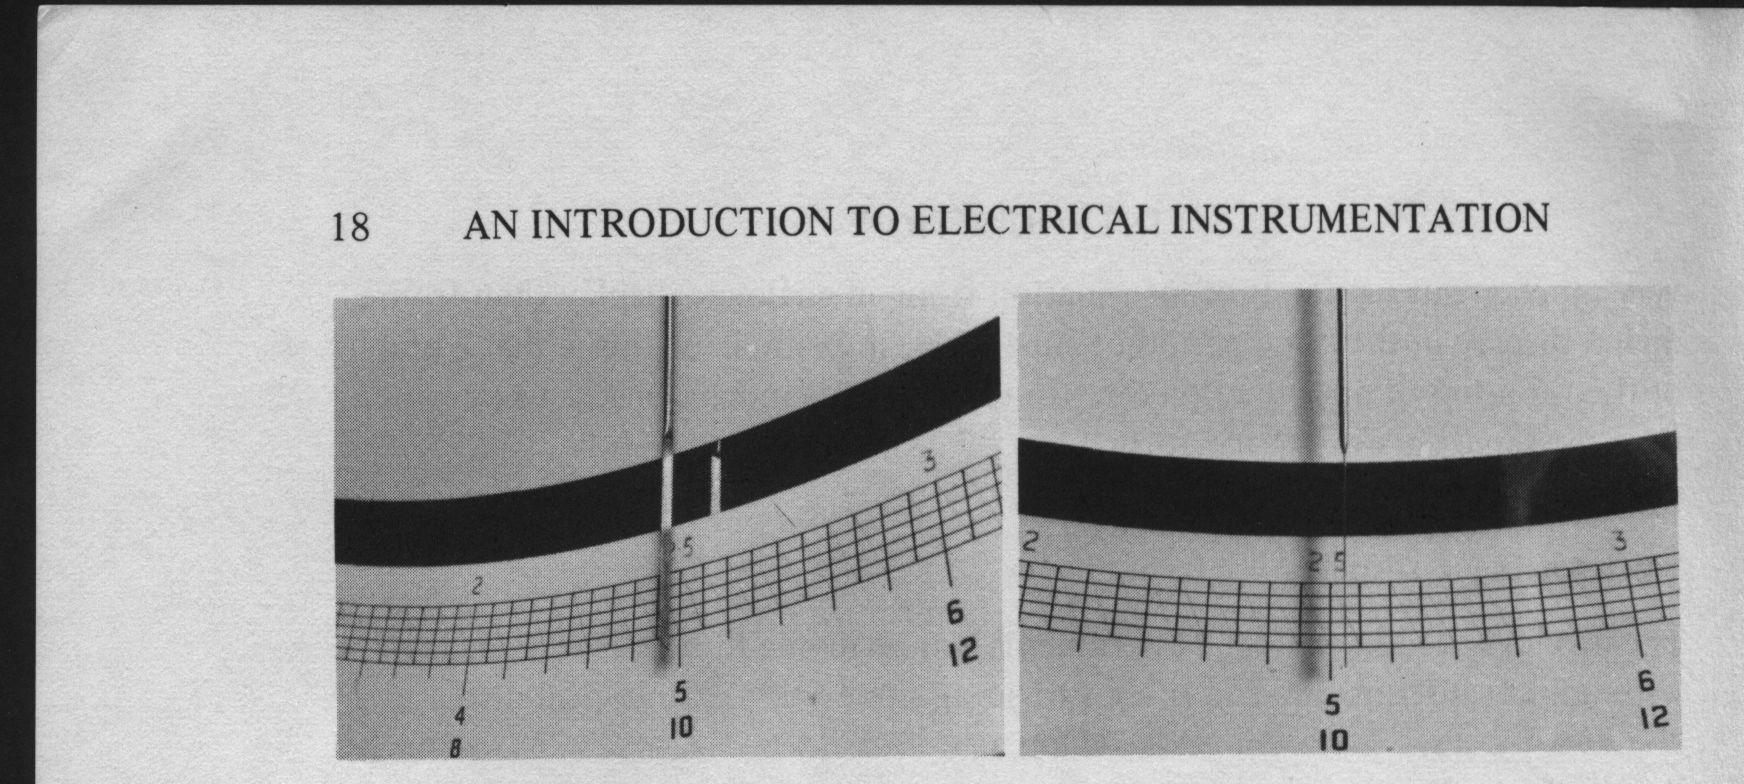
\includegraphics[width=\linewidth]{transparencyPhotoFix}}
		\subbottom[Colocación del papel negro\label{fig:transparencyPaper}]{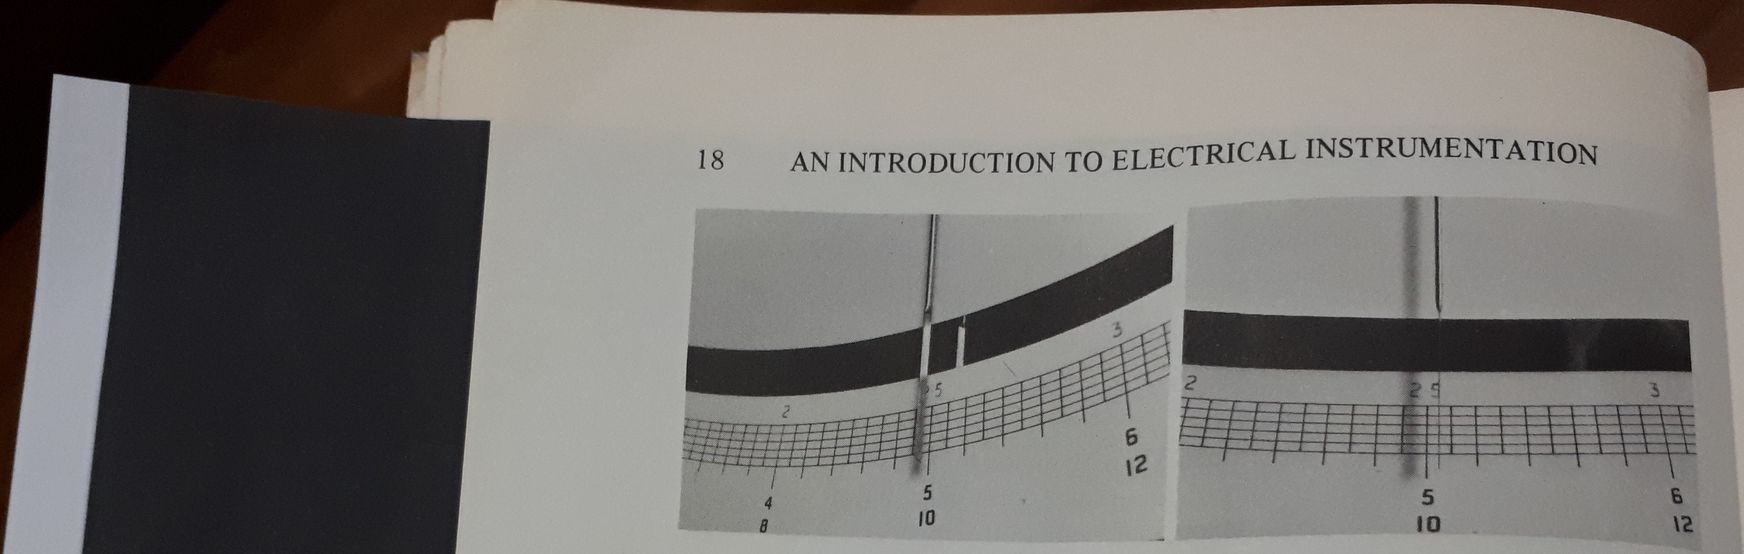
\includegraphics[width=\linewidth]{transparencyPaper}}
		\caption{Detalle de transparencias sobre fotografías impresas\label{fig:transparency}}
	\end{figure}

	\section{Respaldo de los originales\label{sec:scanOriginalBackup}} Al terminar es buena idea hacer un respaldo de las imágenes escaneadas, porque a veces las modificaremos directamente, y podremos evitarnos un disgusto si algo sale mal. Generalmente utilizo \szip para generar un archivo de respaldo con todas. Para hacerlo seleccionamos todos los archivos, hacemos \menu{\rightclick > \szip > Add to archive\...} y elegimos las opciones que deseemos.\footnote{Las opciones por defecto deberían bastar.} El archivo comprimido con los originales podemos guardarlo en la misma carpeta \typesetFolder{SCAN}.

	\section{Conclusiones} En esta sección hemos visto como preparar el escáner y como configurar el software para escanear nuestro material. Se ha usado como ejemplo el software de Epson, pero el aprendizaje debería ser fácilmente trasladable al que tengamos disponible. También vimos como preparar el material a escanear.

	Luego aprendimos sobre el proceso de escaneado en sí, algunos problemas que se pueden presentar y como resolverlos.

	En la sección siguiente veremos como procesar los archivos, separando el texto de las fotografías, de forma de obtener imágenes binarizadas aptas para realizar \ocr.

	\chapter{Limpieza y ajuste\label{sec:cleanAdjust}} Siendo esta la etapa crucial del procesamiento, la presento de la manera más exhaustiva posible. Sin embargo, el detalle que queramos prestarle a cada etapa del procesamiento dependerá de nuestro tiempo, habilidad y paciencia. Algunos de los pasos que siguen podrían ser salteados y aún así obtener resultados aceptables. He tratado de indicarlo cuando así sea.

	\section{Dimensiones\label{sec:cleanAdjustDimensions}} Lo primero que vamos a hacer es medir las dimensiones del libro usando una regla.\footnote{Si el encuadernado fuera tapa dura (\emph{hardback}) tal vez habría un tamaño para las tapas y otro para las páginas. Será nuestra decisión si preservamos esas diferencias o no.} En este caso el ejemplar (tapa blanda) mide 15,5\,cm de ancho, 23,5\,cm de alto y 2,5\,cm de espesor. Al final obtendremos imágenes de 600\,dpi, por lo que podemos convertir entre cm y pixeles usando alguna de las siguientes fórmulas para estimar las dimensiones finales de nuestras páginas procesadas:\footnote{En el apéndice~\ref{app:conversion} se presentan las correspondientes fórmulas en pulgadas.}
	\[
	\text{pix} = \frac{\text{cm} \times \text{dpi}}{\text{2,54}}\hspace{3em} \text{cm} = \frac{\text{pix} \times \text{2,54}}{\text{dpi}}
	\]
	Resumo los resultados en el cuadro~\ref{tab:bookDimensions}.
	\begin{table}
		\centering
		\begin{tabular}{rccc}
			\toprule
			(600\,dpi) & ancho & alto & espesor \\
			\midrule
			cm  & 15,5 & 23,5 & 2,5 \\
			pix & 3661 & 5551 & 591 \\
			\bottomrule
		\end{tabular}
		\caption{Dimensiones del libro a escanear (en cm) y dimensiones estimadas de imagen a 600\,dpi (en pix)\label{tab:bookDimensions}}
	\end{table}

	\section{Orientación de páginas\label{sec:fixOrientation}} De acuerdo a como hayamos colocado el material en el escáner, es posible que las páginas pares o las impares estén rotadas 180\textdegree. Siempre es una buena idea, pero especialmente si estamos pensando en corregir frecuentemente los errores que vayamos encontrando, como se explica en la sección~\ref{sec:SToutput}, que la orientación de todas las páginas originales sea corregida antes de ingresarlas a \scantailor.

	En nuestro caso de ejemplo son las páginas pares las que requieren ajuste. Para hacerlo ejecutamos el script~\ref{scr:orientationOddEven} de Python que invoca el comando \texttt{mogrify} de \imagemagick sobre las páginas de interés. Este nos preguntará por las páginas a corregir (\mintinline{python}|'Rotate odd or even pages?'|): deberemos ingresar \texttt{even} para rotar las pares y \texttt{odd} para las impares. Téngase en cuenta lo dicho en la sección~\ref{sec:scanOriginalBackup} sobre el respaldo de los originales, puesto que con este script los estaremos modificando.

	\pythonScript{orientationOddEven.py}
	\scriptcaption{Rotación de las páginas\label{scr:orientationOddEven}}

	\section{Procesado con \scantailor} Este software es muy completo e incluye una gran cantidad de opciones en sus distintos pasos. La realidad es que al momento de escribir esta guía aún se encuentra pleno en desarrollo, por lo que no existe documentación suficiente que las explique todas en profundidad. Además, algunas son de carácter experimental o directamente no funcionan bien (la función \menu{Dewarp}, por ejemplo). Quien esto escribe no las ha probado todas. Por ello recomiendo al lector que busque la información que necesite en internet\footnote{El autor del fork original tiene una wiki con información y videos \cite{ScanTailorWiki}.} y que no tenga miedo de experimentar.\footnote{\scantailor \emph{no} modifica los archivos originales.} Tal vez esta guía esté sugiriendo algún procedimiento manual tedioso para una tarea que ya está cubierta por una nueva opción. La misma recomendación vale para todo otro software que se utilice.

	\subsection{Creación de un proyecto nuevo} Dicho esto, comenzamos abriendo el software y seleccionando \menu{File > New Project}. Aparecerá un cuadro de diálogo como el de la figura~\ref{fig:STnewProject}, donde elegiremos la carpeta con las páginas escaneadas. Por defecto las imágenes procesadas irán automáticamente a una subcarpeta \typesetFolder{out}. En la columna derecha (\menu{Files In Project}) veremos todos los archivos escaneados. Podríamos excluir algunos seleccionándolos y presionando \keys{«}, pasándolos a la otra columna (\menu{Files Not In Project}). Como la carpeta \typesetFolder{SCAN} es exclusiva para estos archivos, no necesitaremos excluir ninguno.

	\begin{figure}
		\centering
		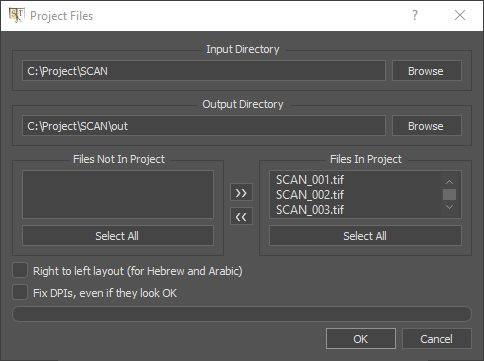
\includegraphics[width=\linewidth]{STnewProject}
		\caption[Cuadro de diálogo New Project, de \scantailor]{Cuadro de diálogo \menu{New Project}, de \scantailor\label{fig:STnewProject}}
	\end{figure}

	\subsection{Paso 1. Fix Orientation\label{sec:STfixOrientation}} Presionamos \keys{OK} y se cargan las imágenes. La vista debería ser como la de la figura~\ref{fig:STfixOrientation}. Sobre la izquierda tenemos el panel \menu{Filters}, con 6 pasos o filtros. Cada uno corresponde a una etapa del proceso. El primero es \menu{Fix Orientation} y se utiliza para corregir la orientación de las imágenes. Si no lo hicimos manualmente como se explica en la subsección~\ref{sec:fixOrientation} debemos hacerlo ahora.

	\begin{figure}
		\centering
		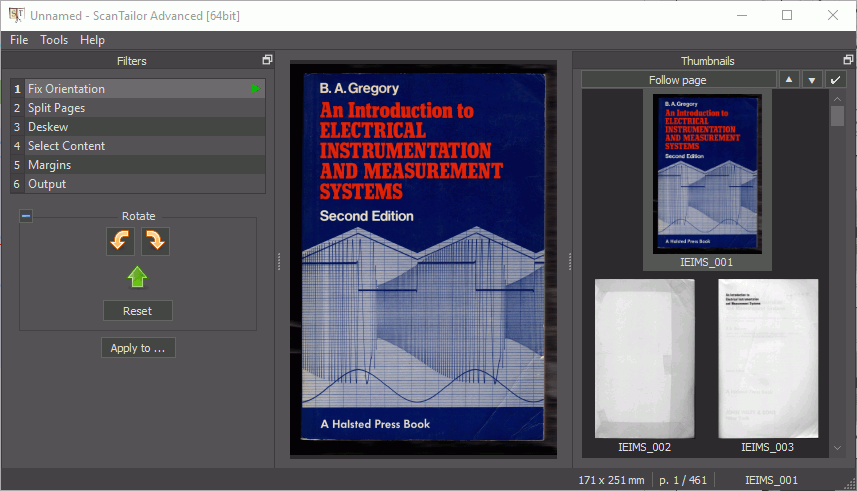
\includegraphics[width=\linewidth]{STfixOrientation}
		\caption[Paso 1: \emph{Fix orientation}]{Ventana principal de \scantailor y Paso 1: \emph{Fix orientation}\label{fig:STfixOrientation}}
	\end{figure}

	Dijimos que teníamos rotadas las páginas pares, por lo que seleccionaremos una cualquiera de estas y presionaremos una de las flechas naranja debajo de \menu{Rotate} hasta que la página quede en la orientación correcta. Una vez listo presionaremos \keys{Apply to\...} y elegiremos la opción \menu{\typesetDotCircle{Every other page}} (fig.~\ref{fig:STfixOrientationApplyTo}). Para ver que más o menos haya quedado bien, podemos recorrer las miniaturas de la columna derecha y verificar que efectivamente todas las páginas están bien orientadas.

	\begin{figure}
		\centering
		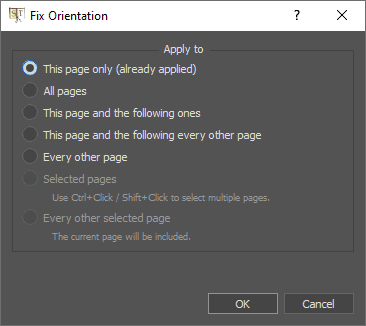
\includegraphics[width=.6\linewidth]{STfixOrientationApplyTo}
		\caption[Cuadro de diálogo \emph{Apply to\...} de \scantailor]{Cuadro de diálogo \menu{Apply to\...} de \scantailor\label{fig:STfixOrientationApplyTo}}
	\end{figure}

	Si la rotación de nuestras exploraciones originales no fuera así de regular, deberemos usar una combinación de rotación manual con opciones del cuadro~\ref{fig:STfixOrientationApplyTo} para asegurarnos de que todas queden con la misma orientación.

	Cuando hayamos terminado presionaremos \play\ a la derecha del nombre del filtro. El programa recorre rápidamente todas las imágenes y genera las miniaturas. Al terminar podemos ir al paso 2.

	\note{Nota: páginas apaisadas} Si bien la mayoría de las páginas tienen orientación vertical, a veces nuestro material contiene algunas páginas con orientación horizontal,\footnote{Ver Wikipedia \cite{WikipediaPageOrientation} (en inglés).} también llamadas páginas «apaisadas» (fig.~\ref{fig:STsplitPagesError}). Más adelante deberemos decidir como queremos que estén en nuestro documento final (sección~\ref{sec:landscapePages}). De momento orientémoslas todas tal como aparecen en el material original.

	\subsection{Paso 2. Split Pages\label{sec:STsplitPages}} En este paso le indicaremos a \scantailor qué parte de la imagen escaneada corresponde a la página. Lo que debemos lograr es que toda la página quede dentro del área azul y que el resto quede fuera: trozos de la hoja que no estábamos escaneando, imágenes de nuestras manos presionando el material, bandas negras donde no había papel, etc.

	En \menu{Page Layout} tenemos tres opciones (fig.~\ref{fig:STsplitPages}). La primera es para indicarle a \scantailor que la página ocupa toda el área de la imagen,\footnote{Útil si ya al escanear dibujamos un rectángulo en el área de previsualización como se explica en la página~\pageref{pag:scanningRegionSelection}.} mientras que la segunda permite excluir dos bandas verticales. Estas dos opciones las usaremos para páginas escaneadas de a una a la vez.

	Si hicimos la digitalización de a dos páginas por vez usaremos la tercera opción, que es la que efectivamente divide la imagen, separándola en dos páginas.\footnote{Téngase en cuenta que si se utiliza esta última opción, cambiará la forma en que \scantailor nombra los archivos de salida y con ello dejará de funcionar el script~\ref{scr:replaceInABBY} de la sección \ref{sec:ABBYCorrectionsSpotAndArea} tal como está.}

	\begin{figure}
		\centering
		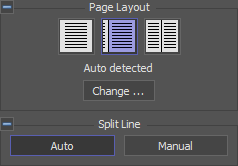
\includegraphics[width=.5\linewidth]{STsplitPages}
		\caption{Paso 2: \emph{Split pages}\label{fig:STsplitPages}}
	\end{figure}

	Cada vez que seleccionamos una página el programa elige automáticamente la opción que considera más adecuada. También podemos presionar \keys{Change\...} y especificar manualmente las opciones para todas las páginas (o pares, impares, etc.).

	Presionamos entonces \play\ para que las analice todas. Luego deberemos recorrerlas y rectificar los errores que encontremos, ya sea cambiando la opción que el programa elige o moviendo la línea por la que se separarán las páginas o recortarán los márgenes. Ver ejemplo en la figura~\ref{fig:STsplitPagesError}.

	\begin{figure}
		\centering
		\subbottom[Error]{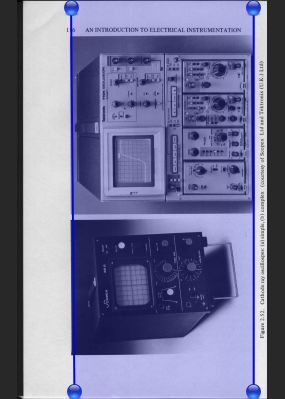
\includegraphics[width=.48\linewidth]{STsplitPagesError}}\hfill
		\subbottom[Remediado]{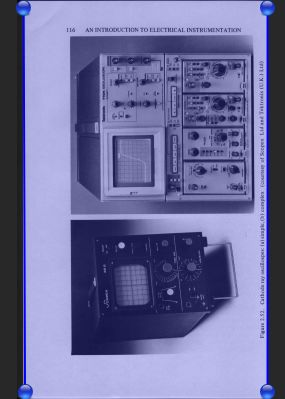
\includegraphics[width=.48\linewidth]{STsplitPagesErrorFix}}
		\caption{Error en el paso 2: Split pages\label{fig:STsplitPagesError}}
	\end{figure}

	\subsection{Paso 3. Deskew\label{sec:STdeskew}} \emph{Deskew} se podría traducir por desinclinar. En este paso el programa analiza cada imagen y corrige la inclinación que pueda tener. Si nuestro trabajo de escaneo fue más o menos prolijo entonces cada imagen necesitará rotarse apenas unos grados o menos. En mi experiencia el algoritmo es bastante robusto y se equivoca poco. De todas formas luego de dar \play\ conviene revisar que esté todo bien.

	\begin{figure}
		\centering
		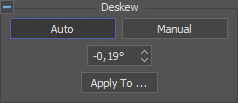
\includegraphics[width=.5\linewidth]{STdeskew}
		\caption{Paso 3: \emph{Deskew}\label{fig:STdeskew}}
	\end{figure}

	El programa ofrece la opción \menu{Order by decreasing deviation}, que permite ordenar las páginas según el ángulo por el cual debieron rotarse. Así ordenadas, las primeras de la lista son las que tienen mayor probabilidad de error, y podemos corregirlas manualmente. En nuestro ejemplo la mayor desinclinación que se debió aplicar fue de solo 1\textdegree. Esto indica que todas las páginas estaban bastante rectas. De todas formas 1\textdegree\ es una cantidad perceptible a simple vista.

	\subsection{Paso 4. Select content\label{sec:STselectContent}} Lo primero que haremos en este paso es indicarle al programa qué tamaño tienen las páginas del material físico y (opcionalmente) donde se encuentran ubicadas en la imagen.

	Lo segundo es parecido al paso 2, solo que ahora se usará un rectángulo para indicar el área de la imagen donde está el contenido. Todo lo que quede fuera de este rectángulo será descartado del resultado final.

	\note{Definición: páginas atípicas} Llamaremos \emph{páginas atípicas} a las correspondientes a las tapas y lomo, así como aquellas páginas que por alguna razón tengan un tamaño físico mayor o menor que el resto, como puede ocurrir con libros que traen páginas dobladas que pueden extenderse. Todas las demás serán, entonces, \emph{páginas típicas}.

	\begin{figure}
		\centering
		\subbottom[Opciones\label{fig:STselectContentOptions}]{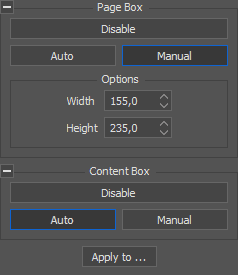
\includegraphics[width=.4\linewidth]{STselectContent}}\hfill
		\subbottom[Diálogo \menu{Apply to\...}\label{fig:STselectContentApplyTo}]{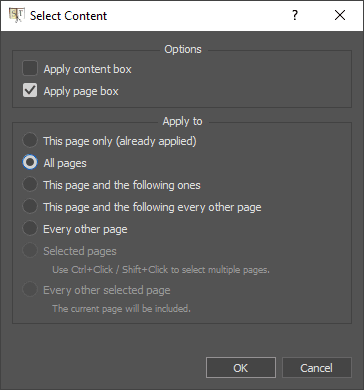
\includegraphics[width=.58\linewidth]{STselectContentApplyTo}}
		\caption{Paso 4: \emph{Select content}\label{fig:STselectContent}}
	\end{figure}

	\subsubsection{Page Box} En el cuadro \menu{Page Box} que se ve en la figura~\ref{fig:STselectContentOptions} presionamos \keys{Manual} e ingresamos respectivamente el ancho y el alto del material en \menu{Width} y \menu{Height} del subcuadro \menu{Options}. En nuestro caso el cuadro~\ref{tab:bookDimensions} de la sección~\ref{sec:cleanAdjustDimensions} nos indica 155\,mm y 235\,mm. Luego presionamos \keys{Apply to\...} y en el cuadro de diálogo que aparece (fig.~\ref{fig:STselectContentApplyTo}) activamos \menu{\typesetCheckbox{Apply page box}} y elegimos \menu{\typesetDotCircle{All pages}}. Finalmente damos \keys{OK} para aplicar las dimensiones ingresadas a todas las páginas del proyecto.

	Como alternativa y si no nos interesa ser muy escrupulosos con las dimensiones originales, podemos elegir \menu{Page Box > \keys{Auto}} y dejar que el programa trate de adivinar el tamaño de cada página y su ubicación. Si procedemos así, entonces podemos saltarnos la sección~\ref{sec:STmarginsOriginals} e ir directo a \ref{sec:STmarginsReasonables}.\todo{Están mal los números de sección.}

	Sea cual sea la opción que elijamos, se generará un rectángulo anaranjado que indica donde \scantailor cree que esta situada la hoja en la imagen y qué tamaño tiene (fig.~\ref{fig:STselectContentError}). Es posible cambiarle el tamaño arrastrando los bordes. Haciendo \keys{\shift + \leftclick + arrastrar} sobre dicho rectángulo podremos posicionarlo correctamente sobre la página.\footnote{Esto solo será necesario si en el paso siguiente (sec.~\ref{sec:STmargins}) usamos la opción \menu{Auto Margins}.}

	Para páginas atípicas recomiendo elegir \keys{Manual} e ingresar las dimensiones manualmente. Si vamos a editar las tapas manualmente como se esboza en la sección~\ref{sec:covers} podemos presionar \keys{Disable}.

	\subsubsection{Content Box} Por defecto, \scantailor trata de detectar las áreas de contenido automáticamente. Para ello usa un algoritmo relativamente lento y propenso a errores, sobre todo si el material contiene manchas, puntos o defectos similares, que puedan ser confundidos con contenido legítimo (fig.~\ref{fig:STselectContentError}). A su vez, tiende a dejar afuera contenido que esté aislado del resto, como pueden ser las cabeceras o pies de página. Por todo esto recomiendo presionar \play\ y después revisar bien.

	\scantailorAdvanced permite hacer \menu{\leftclick\,\leftclick} sobre la imagen para cambiar rápidamente el área de contenido, y así incluir o excluir la zona donde se señaló. También podemos arrastrar los bordes del rectángulo manualmente con \keys{\leftclick + arrastrar} o reposicionarlo con \keys{\shift + \leftclick + arrastrar} (aunque esta última opción no es en general útil).

	Para ayudarnos en la tarea de asegurar el correcto reconocimiento de todas las áreas de contenido también podemos ordenar las páginas: \menu{Order by increasing > width, height, deviation} nos permite agrupar todas las páginas más altas (bajas), más anchas (angostas) o que se desvían más (menos) de la media juntas (fig.~\ref{fig:STselectContentOrder}). En esos conjuntos es más probable encontrar errores.

	\begin{figure}
		\centering
		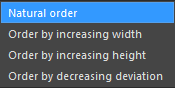
\includegraphics[width=.3\linewidth]{STselectContentOrder}
		\caption{Opciones de ordenación de páginas\label{fig:STselectContentOrder}}
	\end{figure}

	Por ejemplo, en la figura~\ref{fig:STselectContentError} vemos que la página en cuestión era de las más altas no porque el contenido lo fuera, sino porque no había sido correctamente reconocido y debemos arreglarlo.

	\begin{figure}
		\centering
		\subbottom[Error inducido por defectos en la impresión]{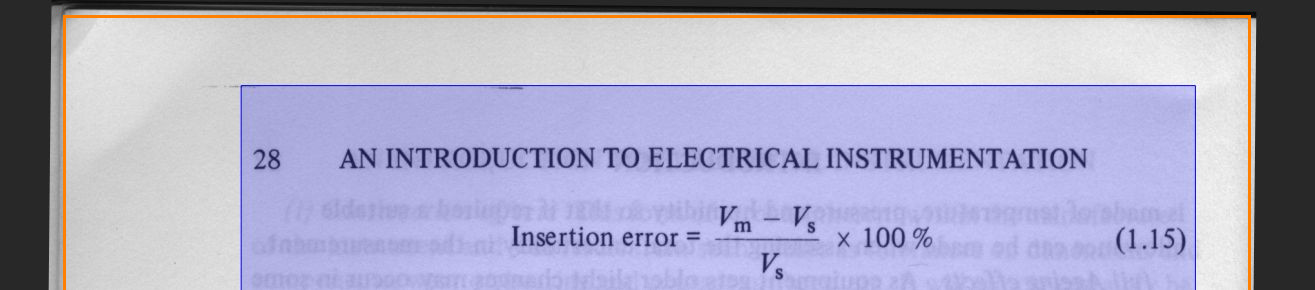
\includegraphics[width=\linewidth]{STselectContentError}}
		\subbottom[Remediado manualmente]{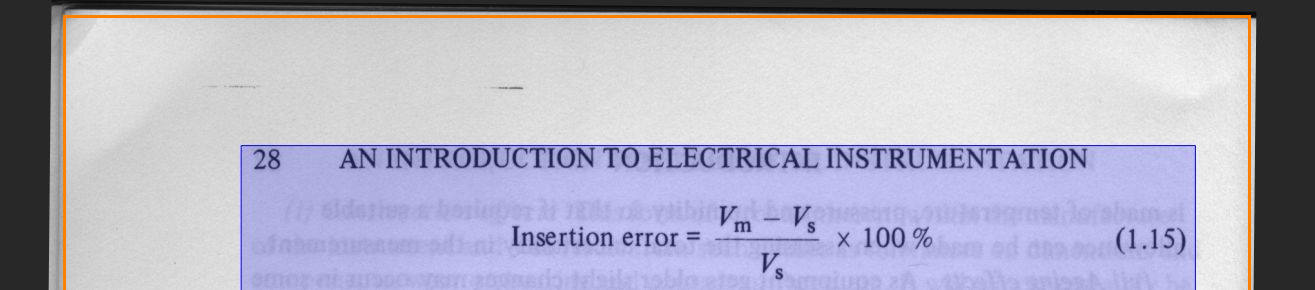
\includegraphics[width=\linewidth]{STselectContentErrorFix}}
		\caption{Error al seleccionar contenido automáticamente\label{fig:STselectContentError}}
	\end{figure}

	En otros casos lo será simplemente porque el contenido va más allá de los márgenes usuales del material, común en libros como el nuestro, con muchos dibujos y diagramas; o simplemente porque la ortotipografía del mismo no fue bien cuidada.\footnote{Como en nuestro material, donde el texto no está justificado.} A veces se encuentran páginas mal desinclinadas o con fotos o diagramas que no fueron correctamente reconocidos como contenido.

	Todos los errores de selección de contenido que no corrijamos seguramente se hagan evidentes al compaginar el documento, sobre todo si somos escrupulosos con los márgenes. En ese punto aún serán fáciles de corregir, pero cuanto menos trabajo nos quede hacia adelante, mejor.

	\subsection{Paso 5. \emph{Margins}\label{sec:STmargins}} Una vez que ya hemos revisado cada página y marcado bien los contenidos es hora de ajustar los márgenes. Propongo un método que conserva lo más exactamente posible la apariencia original y otro que introduce márgenes razonables.

	Cualquiera sea el caso, comenzamos decidiendo respecto a qué parte de las páginas vamos a referir los márgenes. En el caso que nos ocupa, el libro tiene los números de página impresos en las esquinas superiores exteriores de cada hoja. Las pares en la superior izquierda y las impares en la superior derecha. Estos son referencias bastante naturales y son las que usaremos.

	Vamos entonces al paso 5 de \scantailor, nos paramos en una página par y en el submenú \menu{Alignment} (fig.~\ref{fig:STmarginsAlignment}) presionamos la flecha que apunta hacia arriba y a la izquierda. Veremos que la alienación cambia. Por ahora no nos preocuparemos por el ancho de los márgenes. El paso siguiente es presionar \keys{Apply to\...}, seleccionar \menu{\typesetDotCircle{Every other page}} y dar \keys{OK}. Luego hacemos lo mismo con las páginas impares, eligiendo la flecha que apunta hacia arriba y a la derecha.

	\begin{figure}
		\subbottom[Submenú \menu{Margins}\label{fig:STmarginsWidth}]{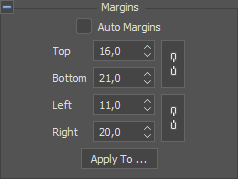
\includegraphics[width=.49\linewidth]{STmarginsWidth}}
		\subbottom[Submenú \menu{Alignment}\label{fig:STmarginsAlignment}]{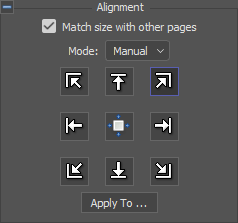
\includegraphics[width=.49\linewidth]{STmarginsAlignment}}\hfill
		\caption{Paso 5: \emph{Margins}\label{fig:STmargins}}
	\end{figure}

	Si nuestra alineación fuera por ejemplo sobre los números de página que aparecen abajo al centro u otra, deberemos elegir la flecha que mejor se ajuste al resultado buscado, tal vez también teniendo que discriminar entre páginas pares e impares.

	Para las páginas atípicas usaremos márgenes especiales, por lo que desactivamos \menu{\typesetBox{Match size with other pages}} para cada una de ellas. Veremos que al hacerlo las dimensiones finales de estas páginas no afectarán a todas las demás.

	Por último activamos la casilla \menu{\typesetCheckbox{Auto Margins}} del menú correspondiente, presionamos \keys{Apply to\...} y elegimos \menu{\typesetDotCircle{All pages}}. Esta opción utilizará la información de \menu{Page Box} y \menu{Content Box} que hayamos ingresado en el paso anterior para generar los márgenes. Para aplicar los márgenes automáticos presionamos \play\ al lado del nombre del filtro.

	\subsubsection{Medida de márgenes originales*} Como muchas veces nuestro material tiene páginas cuyo contenido invade los márgenes, no existe un único valor para el ancho de los márgenes de cada una. En esta subsección opcional veremos una forma de asignar un valor representativo a cada uno de los márgenes.

	\note{Definición: páginas bien comportadas} Dentro del conjunto de páginas típicas, llamaremos páginas \emph{bien comportadas} a aquellas en las que el contenido se mantiene aproximadamente dentro de una misma región. Quedan excluidas de esta definición, y serán por tanto \emph{mal comportadas}, aquellas páginas con imágenes, diagramas, tablas u otros elementos que invaden los márgenes, o aquellas que dan comienzo a un capítulo o sección, entre otras.\todo{Tapas o cubiertas?}

	Comenzando con los márgenes superior e inferior, ordenamos las páginas por alto (\menu{Order by increasing height}) y buscamos abajo del todo la bien comportada más alta. En nuestro caso al final aparecen las tapas (obviamente) y páginas con tablas. La bien comportada más alta es la p.~296. Vamos entonces a esa página en el libro, medimos los márgenes superior e inferior con la regla y los registramos.

	Ahora pasamos a ordenar por ancho: \menu{Order by increasing width}. Hacemos lo mismo que antes, buscamos las bien comportadas más anchas par e impar. Son las pp.~250 y 117. Medimos para cada una el margen izquierdo y derecho y los registramos. Las medidas en este caso se presentan en el cuadro~\ref{tab:pageMargins}.\footnote{Las medidas dieron 20\,mm y 11\,mm para las pares, y 10\,mm y 19\,mm para las impares. Debido a tolerancias de impresión y/o encuadernado las páginas no son simétricas, por lo que las medidas de los márgenes tampoco lo serán exactamente. Para simplificar, haremos que en nuestro resultado sí lo sean, simetrizando estos valores.}

	\begin{table}
		\centering
		\begin{tabular}{@{}rlcccc@{}}
			\toprule
			\multicolumn{1}{c}{página} & \multicolumn{1}{c}{nro.} & sup. & inf. & izq. & der. \\
			\midrule
			alta & p.~296 & 16 & 21 & --- & --- \\
			ancha (par) & p.~250 & --- & --- & 20 & 11 \\
			ancha (impar) & p.~117 & --- & --- & 11 & 20 \\
			\bottomrule
		\end{tabular}
		\caption{Márgenes de las páginas bien comportadas (en mm)\label{tab:pageMargins}}
	\end{table}

	\subsubsection{Márgenes razonables\label{sec:STmarginsReasonables}} Si mantenerse 100\% fiel al material original no es el objetivo, en general la opción \menu{\typesetCheckbox{Auto Margins}} da un buen resultado que además conserva las dimensiones de la página original, por lo que se podría dar aquí por finalizado el paso 5.

	Como alternativa manual, se pueden elegir márgenes arbitrarios (por ej. 10\,mm) o cercanos a los originales, tal vez discriminando un poco para páginas pares e impares (lo mismo respecto de la alineación) y aplicar masivamente a todas las páginas, editando manualmente alguna si así se desea. El resultado dependerá enteramente de nuestro gusto y parecer, pero recomiendo usar los márgenes aproximados del material original al menos como referencia.

	\scantailor por defecto impone el mismo valor para los márgenes izquierdo-derecho y superior-inferior. Si queremos ingresar distintos valores para cada margen debemos presionar \keys{\faLink} a la derecha en la figura~\ref{fig:STmarginsWidth}. Así, la cadena se abre \keys{\faUnlink} y los márgenes ya no tienen por que ser iguales.

	\subsubsection{Conservando la apariencia original\label{sec:STmarginsOriginals}} Si estamos buscando reproducir la apariencia del material original deberemos tener los cuidados que se explican a continuación.

	\paragraph{Alineación} La opción \menu{\typesetCheckbox{Auto Margins}} nos asegura un tamaño de página correcto, pero aún falta alinear los contenidos. Podríamos dejarlo así, pero quedaría mejor si todos los números de página ocuparan la misma posición en todas las páginas, independientemente de que haya contenido que invada los márgenes. Para hacer este ajuste, \scantailorAdvanced ofrece las así llamadas \emph{guides} (fig.~\ref{fig:STmarginsGuides}), que pueden ser verticales u horizontales.

	\begin{figure}
		\tiny
		\def\svgwidth{\linewidth}
		\subbottom[Página par]{\input{img/STmarginsEven.pdf_tex}}
		\def\svgwidth{\linewidth}
		\subbottom[Página impar]{\input{img/STmarginsOdd.pdf_tex}}
		\caption[Detalle de las guías para ajustar márgenes]{Detalle de las guías para ajustar márgenes. Las páginas (bien comportadas) ya fueron alineadas con sus guías correspondientes\label{fig:STmarginsGuides}}
	\end{figure}

	Para crearlas hacemos \menu{\rightclick > Add vertical guide}, y las posicionamos con \keys{\ctrl + \Alt + \leftclick + arrastrar}. Haciendo \keys{\shift + \leftclick + arrastrar} podemos mover el contenido en sentido horizontal para alinearlo. En este caso será al número de página. Necesitaremos una para las pares y otra para las impares. Sugiero fijar las guías en las páginas más anchas (pp.~250 y 117).\todo{Referir a la documentación de \scantailor para los controles.}

	Con \keys{\shift + \,\leftclick\,\leftclick} sobre el área que queremos alinear, \scantailor hace un buen trabajo de acomodar automáticamente el contenido a la guía más cercana. Si no nos satisface el resultado, podemos arrastrarlo manualmente como en el párrafo anterior, hasta colocarlo donde queramos.

	Si también quisiéramos ajustar la posición vertical, crearíamos una guía horizontal con \menu{\rightclick > Add horizontal guide} y usaríamos \keys{\ctrl + \,\leftclick\,\leftclick} o \keys{\ctrl + \leftclick + arrastrar} para alinear el contenido verticalmente. Podría ponerse esta guía en los títulos de página, en cuyo caso la crearíamos con la página más alta como referencia. En este caso considero que no es necesario ajustar verticalmente las páginas bien comportadas.

	Como todos los comienzos de capítulos omiten el número de página, debemos usar otro punto como referencia. Elegí la base del texto que marca el título. Es la única guía horizontal que creé para este proyecto.

	Algunas páginas mal comportadas podrían alinearse sin la necesidad de guías. Bastará con medir los márgenes e ingresarlos manualmente, desactivando \menu{\typesetBox{Auto Margins}}. Estoy pensando en las portadillas, portadas, colofones, etc.

	Para sacar provecho de este método debemos avanzar manualmente página por página, alineando el contenido a las guías. Este puede tomar algo de tiempo y según el caso podría no ser necesario o no valer la pena.

	\paragraph{Verificación} Si nos interesa verificar que los márgenes nos hayan quedado bien, podemos usar \djvusmall\footnote{Para aprender a trabajar con \djvusmall consultar la sección~\ref{sec:djvuSmall}.} con un perfil cualquiera (por ejemplo, \menu{default}) para generar un \djvu de prueba y, pasando las páginas rápidamente, detectar algún error de alineación que no hayamos notado. También es posible ir pasando dentro de \scantailor, pero de momento la navegación es bastante lenta y a veces no permite apreciar las diferencias.

	\subsection{Paso 6. \emph{Output}\label{sec:SToutput}} Comenzaremos por seleccionar \menu{Output Resolution (DPI) > 600} y presionamos \play\ para que se binaricen todos los archivos. Este es un proceso que también le lleva a \scantailorAdvanced algo de tiempo, aunque se ha mejorado mucho respecto de la versión original. Al finalizar podemos inspeccionar cada página en busca de errores. A continuación veamos algunos de los más comunes.

	\subsubsection{Caracteres mal impresos o faltantes} A veces el proceso de impresión falla y algunos caracteres aparecen cortados, como en la figura~\ref{fig:SToutputBadChars}. Existen dos formas de corregirlos.
	\begin{enumerate}
		\item Usando \gimp para editar los originales. Tenemos la herramienta pincel para corregir errores o podemos copiar caracteres buenos y pegarlos sobre los que tienen problemas. Es bastante versátil pero requiere ubicar el archivo, cargarlo, editar la imagen, guardarla, ver el resultado en \scantailor y quizás repetir. %rinse and repeat
		\item Usando la pestaña \menu{Fill zones} de \scantailor. Allí podemos dibujar regiones (poligonales) para que el programa rellene. Haciendo \menu{\rightclick > Pick color} sobre ellas elegimos el color para rellenar (generalmente blanco o negro).
	\end{enumerate}

	\begin{figure}
		\subbottom[Original]{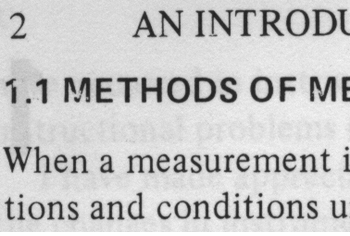
\includegraphics[width=.32\linewidth]{SToutputBadCharsOriginal}}\hfill
		\subbottom[Salida]{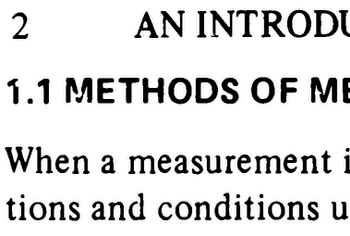
\includegraphics[width=.32\linewidth]{SToutputBadChars}}\hfill
		\subbottom[Salida corregida]{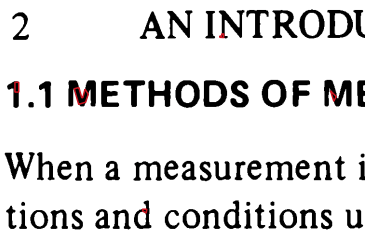
\includegraphics[width=.32\linewidth]{SToutputBadCharsFix}}
		\caption[Caracteres cortados]{Caracteres cortados. La corrección se hizo desde la pestaña \menu{Fill zones}\label{fig:SToutputBadChars}}
	\end{figure}

	Dependiendo de la cantidad y gravedad de estos errores valdrá la pena invertir el tiempo y repararlos o simplemente dejarlos así. %let them be
	Si los originales tienen problemas hay un límite en la cantidad de esfuerzo que podemos echarle para mejorarlos. No hay que ser más papista que el papa. %theres only so much we can do

	\subsubsection{Motas y manchas no detectadas} Una de las opciones que tiene al etapa 6 se llama \emph{despeckle}, que podría traducirse como eliminación de motas. Lo que hace es buscar puntos pequeños y generalmente aislados, que probablemente no sean parte del contenido, sino más bien problemas de impresión o escaneo (motas de polvo).

	Funciona bastante bien, salvo en dos casos: si los puntos son demasiado grandes (fig.~\ref{fig:SToutputDespeckleSpot}) o si están entremezclados con el resto del contenido (fig.~\ref{fig:SToutputDespeckleSpeckle}). En ambos se puede corregir manualmente, ya sea usando \gimp o \menu{Fill zones}.

	También existe la posibilidad de cambiar el parámetro del filtro, para que detecte detalles más grandes. En dicho caso se debe tener cuidado de que no elimine elementos que no debe, como por ejemplo puntos y comas.

	\begin{figure}
		\subbottom[Original\label{fig:SToutputDespeckleSpotOriginal}]{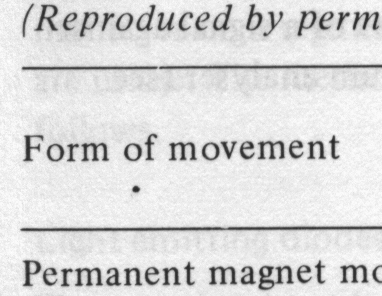
\includegraphics[width=.48\linewidth]{SToutputDespeckleSpotOriginal}}\hfill
		\subbottom[Procesada. Punto no eliminado\label{fig:SToutputDespeckleSpotBad}]{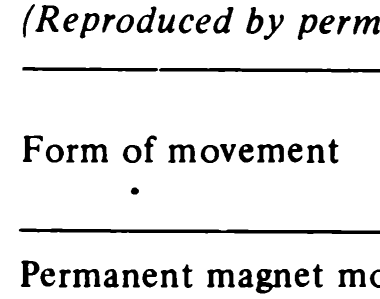
\includegraphics[width=.48\linewidth]{SToutputDespeckleSpotBad}}
		\caption{Filtro \emph{despeckle} frente a puntos demasiado grandes\label{fig:SToutputDespeckleSpot}}
	\end{figure}

	\begin{figure}
		\subbottom[Original. Dos motas\label{fig:SToutputDespeckleSpeckleSomeOriginal}]{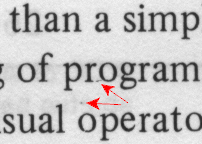
\includegraphics[width=.48\linewidth]{SToutputDespeckleSpeckleSomeOriginal}}\hfill
		\subbottom[Procesada. Una mota permanece\label{fig:SToutputDespeckleSpeckleSome}]{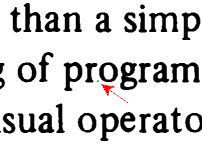
\includegraphics[width=.48\linewidth]{SToutputDespeckleSpeckleSome}}
		\caption{Filtro \emph{despeckle} frente a motas pegadas al texto\label{fig:SToutputDespeckleSpeckle}}
	\end{figure}

	\subsubsection{Contenido por motas} A veces al \emph{despeckle} se le va la mano y borra puntos que en realidad pertenecen al contenido. Ver la figura~\ref{fig:SToutputDespeckle}. Si interesa retener esos puntos podría desactivarse el filtro y hacer un \emph{despeckle} manual en esa página. Otra alternativa puede ser darle énfasis a los puntos de interés con el \gimp, para que el filtro no los borre (es lo que se hizo en este caso).

	\begin{figure}
		\subbottom[Original]{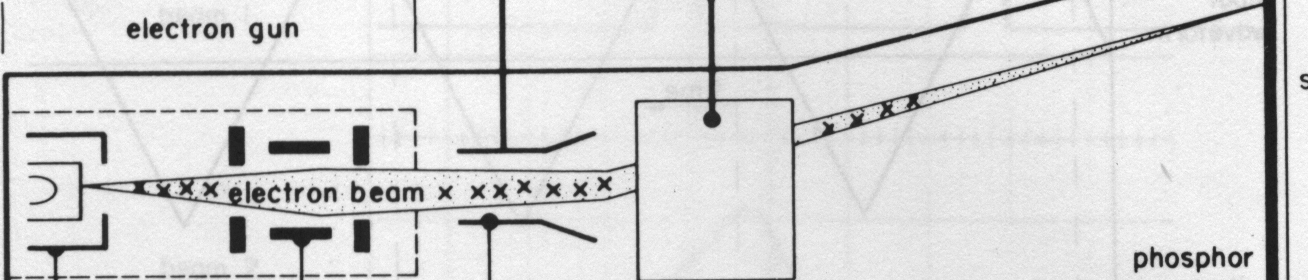
\includegraphics[width=\linewidth]{SToutputDespeckleOriginal}}
		\subbottom[Procesada]{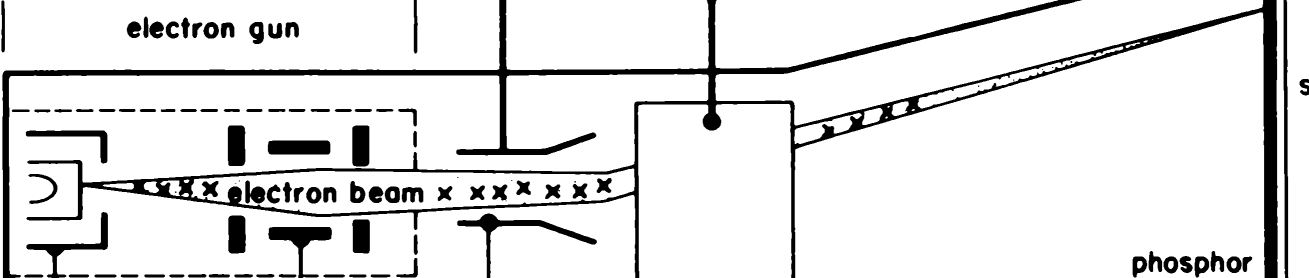
\includegraphics[width=\linewidth]{SToutputDespeckleBad}}
		\subbottom[Procesada luego de dar énfasis con \gimp]{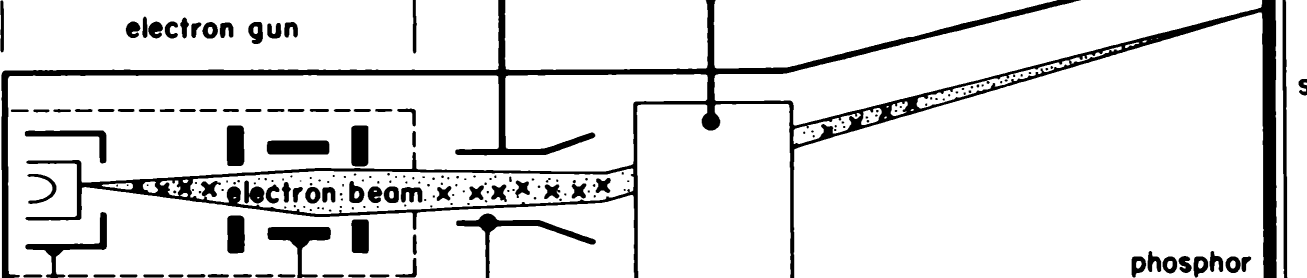
\includegraphics[width=\linewidth]{SToutputDespeckleFix}}
		\caption{Efecto indeseado del filtro despeckle\label{fig:SToutputDespeckle}}
	\end{figure}

	\subsubsection{Desinclinación incorrecta} Si bien este error debió comentarse en la sección~\ref{sec:STdeskew}, al menos a mí me sucede que no lo detecto hasta este paso.

	Se trata de páginas que no se rotaron el ángulo correcto. En mi experiencia, sucede principalmente en dos casos:
	\begin{enumerate}
		\item Páginas apaisadas. Nuestro libro tiene varias tablas grandes y páginas con figuras que se imprimieron rotadas para que quepan mejor en la hoja. Deberemos ajustar el ángulo manualmente.\footnote{Téngase en cuenta lo que se explica en la sección~\ref{sec:landscapePages}.}
		\item Páginas con contenido a distintos ángulos. En nuestro libro sucede que algunos dibujos consisten en líneas rectas no paralelas al texto. Esto puede confundir al algoritmo. En otros casos podría haber texto escrito a distintos ángulos, ya sea de manera intencional o por errores en la composición de la página. Dependiendo del caso, podemos ajustar el ángulo manualmente o usar la herramienta de rotación de \gimp para alinear solo aquella parte de la página que no lo esté.
	\end{enumerate}

	\subsubsection{Picture zones\label{sec:SToutputPictureZones}}

	Para las páginas que además del texto tengan fotos que queramos preservar, deberemos elegir la opción \menu{Mode > Mixed}.\footnote{Este es el método que recomiendo para trabajar con las páginas con ilustraciones de nuestro material. Algunas alternativas no recomendadas se discuten en el apéndice~\ref{sec:noSplitPages}.} La opción por defecto es \menu{Black and White}, que binariza todo, y la restante, \menu{Color / Grayscale}, retiene la página original completa, salvo por los efectos de los pasos anteriores.

	Eligiendo \menu{Mixed} el software intentará adivinar las áreas donde se encuentran las fotos. En la pestaña \menu{Picture Zones} se señalan titilando con color azul. Por defecto estas áreas pueden tener cualquier forma, pero seleccionando \menu{Picture Shape > Rectangular} (fig~\ref{fig:SToutputPicureZonesRectangular}) podemos forzar a que sea rectangular, que servirá en la mayoría de los casos.

	\begin{figure}
		\centering
		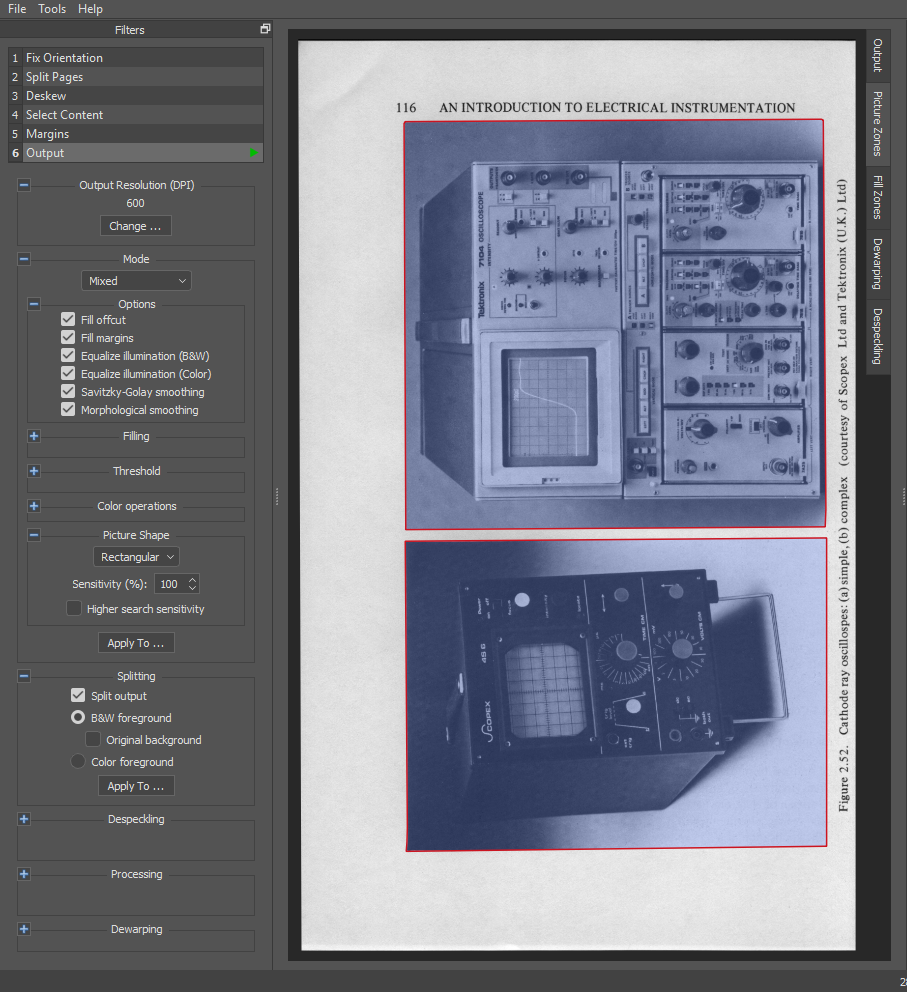
\includegraphics[width=\linewidth]{SToutputPicureZonesRectangular}
		\caption[Paso 6: \emph{Output}]{Paso 6: \emph{Output}. Se seleccionó la pestaña \menu{Picture zones}\label{fig:SToutputPicureZonesRectangular}}
	\end{figure}

	En los que no, deberemos dibujar nuestras propias zonas (y tal vez eliminar o corregir algunas mal detectadas). Para cada una podemos hacer \menu{\rightclick > Properties} y elegir si añadirla a la capa ya detectada (\menu{Add to auto layer}), eliminarla de esa capa (\menu{Subtract from auto layer}) o eliminarla de todas las capas (\menu{Subtract from all layers}). Todo esto tendrá sentido si las zonas se superponen. Sugiero experimentar un poco con las opciones para entender bien su significado.

	Un ejemplo de zonas dibujadas manualmente y su resultado se muestra en la figura~\ref{fig:SToutputPicureZonesFree}. Nótese que es posible tener huecos dentro de la foto que serán rellenados de blanco. En este caso le darán un efecto interesante al resultado final. De lo contrario esos huecos quedarían rellenos con el color del blanco de la página, que como se ve en la figura \ref{fig:SToutputPicureZonesFreeOriginal} es más bien un beige.

	\begin{figure}
		\subbottom[Zonas marcadas manualmente\label{fig:SToutputPicureZonesFreeOriginal}]{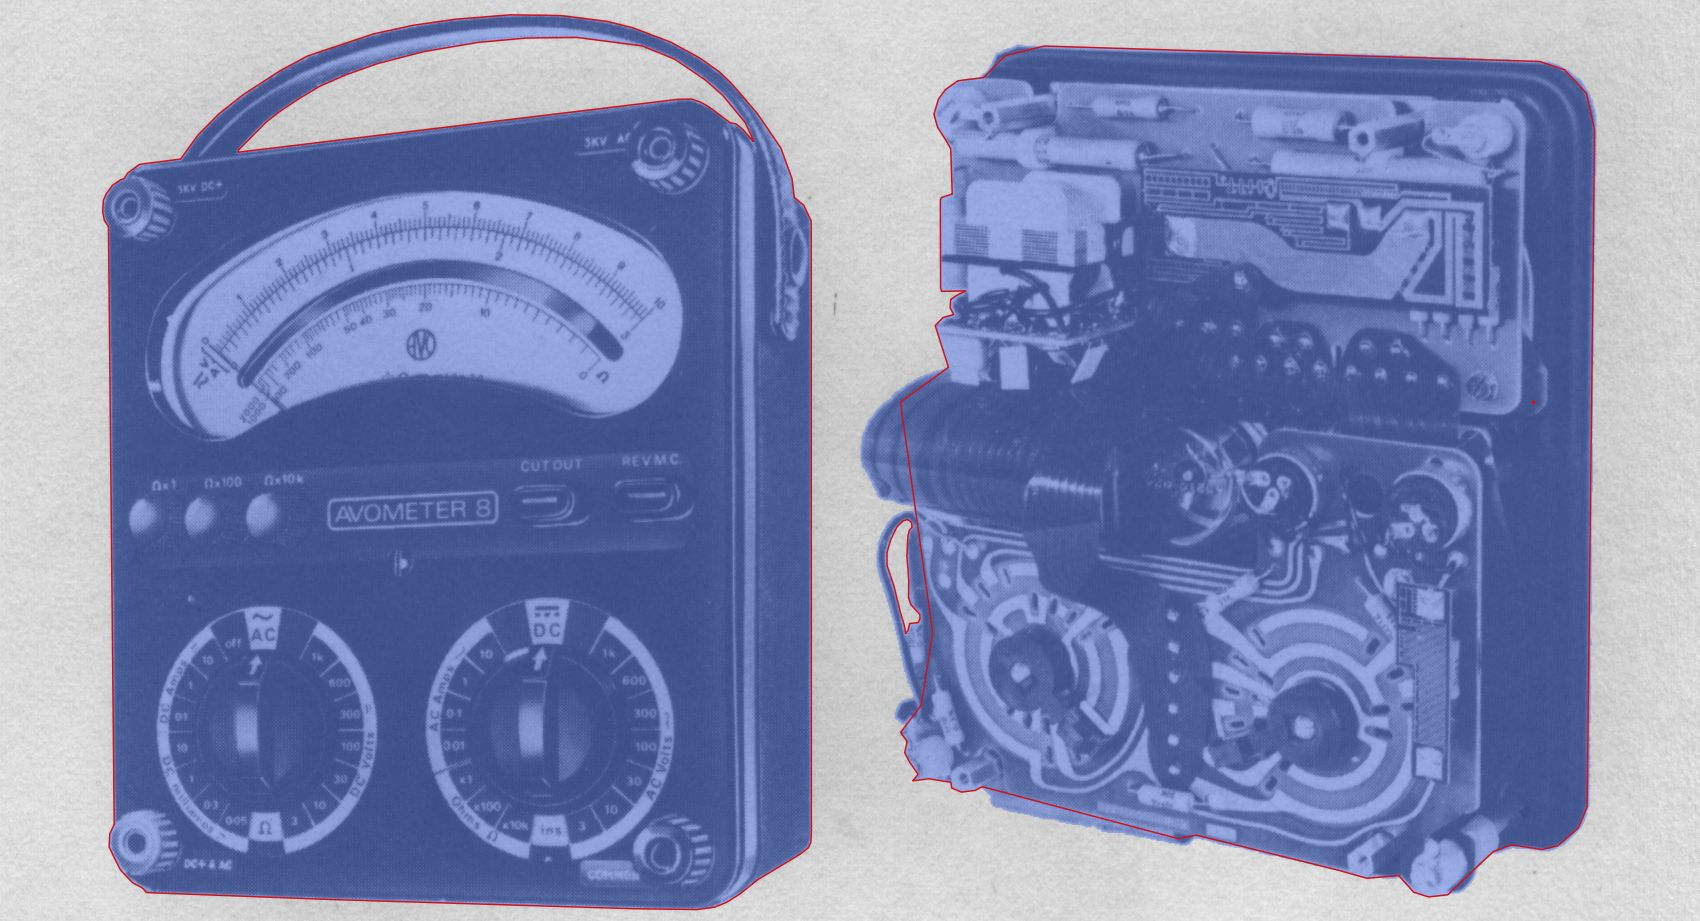
\includegraphics[width=\linewidth]{SToutputPicureZonesFree}}
		\subbottom[Resultado]{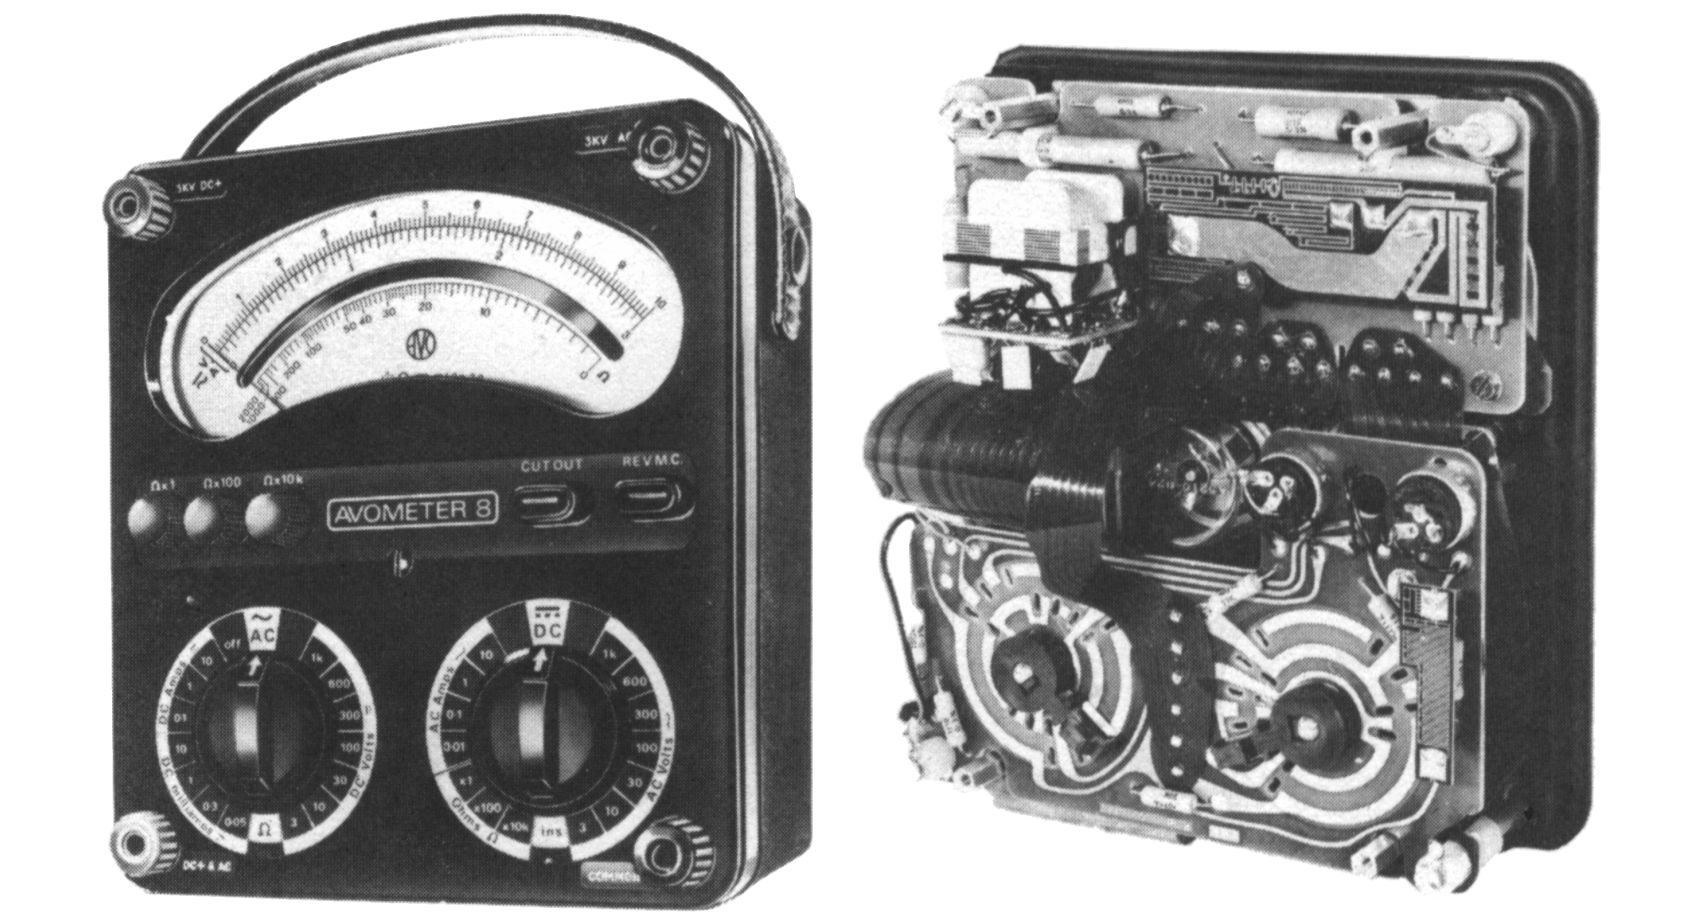
\includegraphics[width=\linewidth]{SToutputPicureZonesFreeResult}}
		\caption[Selección manual de las fotos en pestaña Picture Zones]{Selección manual de las fotos en pestaña \menu{Picture Zones}. Los contornos rojos se dibujaron manualmente\label{fig:SToutputPicureZonesFree}}
	\end{figure}

	Una opción a tener en cuenta y que me ha dado buenos resultados es \menu{Options > Equalize illumination (Color)}.

	Para estas páginas debemos activar siempre \menu{Splitting > Split output > \typesetCheckbox{B\&W foreground}}. Esto generará dos carpetas más dentro de \typesetFolder{out}: \typesetFolder{foreground} y \typesetFolder{background}, adonde se guardará cada componente de la imagen. A la primera irá todo el contenido binarizado y a la segunda las fotos. Podemos activarla y echar un vistazo para entenderlo mejor.

	Esto nos permitirá procesar cada parte en sus particularidades de manera independiente, de forma de lograr un resultado óptimo. Si no se va a hacer, de todas formas elegir la opción no hace daño, pues en \typesetFolder{out} se sigue guardando la imagen con las dos componentes superpuestas.

	\subsubsection{Ilustraciones problemáticas} Algunas ilustraciones, dibujos o diagramas, a pesar de estar impresos a una sola tinta, pierden muchos detalles cuando son binarizados. Ocurre cuando hay líneas muy cercanas pero que no se tocan: el blanco que queda en medio no es lo suficientemente claro, y \scantailor lo convierte en negro. Análogamente si hay líneas negras demasiado tenues. La figura~\ref{fig:SToutputBadDiagrams} ilustra un ejemplo. Para arreglar esto existen tres opciones.

	\begin{enumerate}[noitemsep]
		\item La más sencilla es tratarlos como fotos. Procedemos exactamente como se explicó en la sección~\ref{sec:SToutputPictureZones}.
		\item Si se dispone de un poco más de tiempo, se pueden editar con \gimp para generar un contraste mayor que permita una binarización más efectiva. Para ello se pueden usar filtros o manualmente redibujar los detalles que se quieran conservar.
		\item La tercera consiste en ajustar el algoritmo de binarización, como se explica a continuación. Tiene el inconveniente de que los cambios afectan a toda la página y no solo al dibujo de interés, lo que podría generar discordancias visibles con el resto de las páginas que usen los valores por defecto u otros.
	\end{enumerate}

	\begin{figure}
		\hspace*{\fill}
		\subbottom[Exploración original]{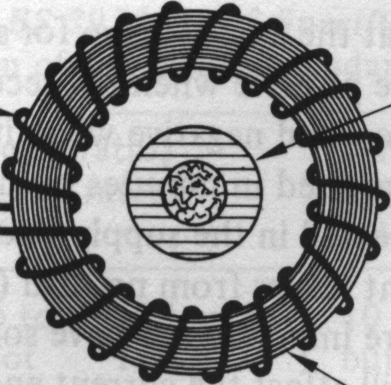
\includegraphics[width=.4\linewidth]{SToutputBadDiagramsOriginalScan}}\hfill
		\subbottom[Salida original]{\includegraphics[width=.4\linewidth]{SToutputBadDiagramsOriginalOutput}}\hspace*{\fill}\\
		\hspace*{\fill}
		\subbottom[Corregida (manualmente)]{\includegraphics[width=.4\linewidth]{SToutputBadDiagramsCorrectedScan}}\hfill
		\subbottom[Salida final]{\includegraphics[width=.4\linewidth]{SToutputBadDiagramsCorrectedOutput}}%
		\hspace*{\fill}
		\caption{Binarización de una ilustración problemática\label{fig:SToutputBadDiagrams}}
	\end{figure}

	\subsubsection{Algoritmo de binarización} Existen diferentes algoritmos de binarización, cada uno con ventajas y desventajas. Con el submenú \menu{Threshold} (umbral) \scantailorAdvanced permite cambiar entre \menu{Otsu} (por defecto), \menu{Sauvola} y \menu{Wolf}. De no estar conformes con el resultado por defecto, podríamos intentar cambiando el algoritmo o ajustando los parámetros que cada uno ofrece. El impacto que tiene cada algoritmo está por fuera del alcance de nuestra guía, si bien existe abundante literatura al respecto \cite{RashmiBinarization}.

	\subsection{Páginas apaisadas\label{sec:landscapePages}} Recomiendo corregir la rotación de las páginas apaisadas (\emph{landscape}, en inglés) para que estén bien orientadas en el documento final (fig.~\ref{fig:STlandscapePages}). De esta forma se facilita el \ocr y queda más fácil de visualizar. Si bien podríamos haber elegido la orientación adecuada desde el paso 1 de \scantailor, no lo hacemos así porque no tener todas las páginas orientadas en el mismo sentido nos dificulta la configuración de márgenes consistentes.\footnote{En realidad, nos obliga a considerar todas esas páginas como atípicas, teniendo que ingresar todos sus márgenes manualmente.} Por ello, debemos tomar nota de los números de página que queramos ajustar y adaptar el script~\ref{scr:fixLandscapePages} para que las procese correctamente.\footnote{Bastará con rellenar la variable \menu{landscapePages} con los números de página correspondientes.}

	\begin{figure}
		\includegraphics[width=\linewidth]{STlandscapePages}
		\caption{Página apaisada y sus contiguas en el documento final\label{fig:STlandscapePages}}
	\end{figure}

	\pythonScript{fixLandscapePages.py}
	\scriptcaption{Ajuste de páginas apaisadas\label{scr:fixLandscapePages}}


	\section{Tapas\label{sec:covers}} Las tapas de los libros muchas veces son las únicas ilustraciones o fotografías a color que que estos incluyen, por lo que me gusta dedicarles un poco más de atención.

	En la figura~\ref{fig:SCANcoverRaw} vemos la tapa del libro sobre el que estamos trabajando. Consta básicamente de 4 colores: blanco para el nombre del autor y la edición, naranja para el título de la obra, azul oscuro para el fondo y los gráficos de la parte de abajo y azul celeste para el fondo del gráfico. Podemos ver que en las esquinas presenta marcas de doblez y que en algunos lugares se ha borrado la ilustración.

	Para remediar estos detalles uso \gimp. El proceso cae un poco por fuera de los objetivos de esta guía, así que no entraré en pormenores. Valga decir que selecciono las áreas de cada color y las vuelvo uniformes, para luego convertir la imagen en indizada. De esta manera conservo el diseño original y reduzco el tamaño casi 100 veces. La diferencia se muestra en la figura~\ref{fig:SCANcover}. Este archivo, que es una modificación de lo que entrega \scantailor, debemos guardarlo en una carpeta aparte, para que el programa no lo sobrescriba accidentalmente.

	\begin{figure}
		\centering
		\subbottom[Escaneo crudo\label{fig:SCANcoverRaw}]{\includegraphics[width=.48\linewidth]{SCANcoverRaw}}\hfill
		\subbottom[Retocado\label{fig:SCANcoverMOD}]{\includegraphics[width=.48\linewidth]{SCANcoverMOD}}
		\caption[Efectos de retoque en la tapa del libro]{Efectos de retoque en la tapa del libro. Se pasó de un \tiff de 56\,MB a uno de 0,69\,MB con una apariencia más limpia\label{fig:SCANcover}}
	\end{figure}

	Las cubiertas con diseños más complejos o que incluyen fotos no admiten el mismo tipo de edición, aunque muchas veces es posible mejorarlas ajustando brillo, contraste, etc. Si bien la tapa es la presentación del libro, el peso en el tamaño final no debería ser excesivo.

	\subsection{Nota: sobre la fidelidad de los colores} No tiene mucho sentido obsesionarse con que los colores se vean exactamente igual que en el material físico.

	Tengamos en cuenta que si nuestro monitor no está calibrado, los colores que estamos viendo en él no se corresponderían con los que se verían por ejemplo si se mandara a imprimir lo que tenemos en frente. No olvidemos que estamos digitalizando un documento, por lo que estamos pensando en visualizarlo luego en una pantalla. Distintas personas verán distintos colores en distintos monitores. No hay remedio para esto.

	\section{Conclusiones} En este capítulo hemos visto como procesar nuestras páginas escaneadas a través de los distintos pasos de \scantailor, de manera de obtener resultados que reflejen adecuadamente las características del material original. Para ello debemos obtener información del mismo, por lo que será bueno tenerlo a mano mientras trabajamos. También comentamos algunas ideas sobre el procesamiento de las tapas.

	En el siguiente capítulo trabajaremos con la salida de \scantailor para reconocer el texto. Esto le agregará mucho valor al resultado final, por la posibilidad de hacer búsquedas.

	\chapter{\texorpdfstring{\textsc{Ocr}}{OCR} con \abby\label{sec:OCR}} Una vez que las páginas fueron limpiadas y ajustadas y las fotos separadas, podemos proceder a realizar el reconocimiento de texto. Como paso previo, notemos que que si marcamos \menu{Picture zones} y elegimos la opción \menu{Split output}, tenemos en la carpeta \typesetFolder{out} las imágenes procesadas y dentro de la misma otras dos carpetas, como se explicó antes.

	Debemos ahora copiar las imágenes desde \typesetFolder{foreground} a la carpeta \typesetFolder{out} y sobrescribir los archivos. Así, en \typesetFolder{out} habrá solo imágenes binarias (texto y diagramas monocromáticos). Las fotos quedarán en \typesetFolder{background} y trabajaremos sobre ellas más adelante.

	Lo mismo haremos con las tapas si las procesamos aparte. Las copiamos a la carpeta \typesetFolder{out}, sobrescribiendo las que generó \scantailor. De esta manera tendremos en \typesetFolder{out} las páginas que conformarán el documento final (salvo las fotos).

	\note{Nota previa} \abby también es un programa muy completo, con una cantidad de modos de funcionamiento, opciones y errores que esta guía no pretende cubrir exhaustivamente. Si alguna explicación no quedara clara, lo mejor será experimentar, leer el manual de usuario o realizar consultas en algún sitio especializado.

	\section{Configuración} Abrimos luego el \abby\footnote{Recomiendo trabajar con la versión 14 (la más reciente al momento de escribir esta guía). Sin embargo, cualquier versión que permita salvar en \djvu es suficiente (v11 o superior). Las opciones no serán exactamente iguales (habrá que improvisar) y no podremos usar el script~\ref{scr:replaceInABBY} (no es grave).} y procedemos a configurar primero las opciones básicas (más adelante trataremos algunas otras). Se accede al menú haciendo \menu{\leftclick > Tools > Options}. En principio sugiero configurar las opciones tal cual se muestran en las figuras.

	\subsection{Pestaña \texttt{Image Processing}} En la pestaña \menu{Image Processing} presionamos \keys{Show Advanced Settings} y deshabilitamos todas las opciones, como en la fig.~\ref{fig:ABBYoptionsImage}. Así nos aseguramos de que el software no realizará ninguna corrección de imagen. Para eso ya transitamos por los pasos anteriores. Si aún hubiera algo para ajustar, lo mejor será volver a \scantailor y hacerlo nosotros mismos.

	\begin{figure}
		\centering
		\includegraphics[width=\linewidth]{ABBYoptionsImage}
		\caption[Opciones de \abby. Pestaña Image Processing]{Opciones de \abby. Pestaña \menu{Image Processing}\label{fig:ABBYoptionsImage}}
	\end{figure}

	\subsection{Pestaña \texttt{Languages}} Pasamos ahora a la pestaña \menu{Languages} (fig.~\ref{fig:ABBYoptionsLanguages}) donde crearemos primero un nuevo idioma basado en uno ya existente. Esto lo hacemos así si nuestro material contiene caracteres de otro alfabeto, por ejemplo el griego. O si queremos editar los caracteres permitidos para ayudar con el reconocimiento.\footnote{A veces el programa confunde un carácter por otro. Muy comúnmente «\textit{l}» cursiva por «/». Si este último no es usado en nuestro material, podemos eliminarlo de la lista de caracteres permitidos para forzar al programa a intentar reconocer otro carácter. Esto no garantiza resultados (podría aun confundirlo con «|», por ejemplo), pero puede ayudar.}

	\begin{figure}
		\centering
		\includegraphics[width=\linewidth]{ABBYoptionsLanguages}
		\caption[Opciones de \abby. Pestaña Languages]{Opciones de \abby. Pestaña \menu{Languages}\label{fig:ABBYoptionsLanguages}}
	\end{figure}

	Elegimos \menu{\typesetDotCircle{Specify OCR languages manually}}, presionamos \keys{New} y seleccionamos \menu{\typesetDotCircle{Create a new language based on\...}} (fig.~\ref{fig:ABBYoptionsLanguagesNewLanguage}). En este caso elegimos \menu{English}, presionamos \keys{OK}, le ponemos por nombre \menu{MyEnglish} y damos \keys{OK} nuevamente (fig.~\ref{fig:ABBYoptionsLanguagesLanguageProperties}). Al final deberá decir \menu{\typesetDotCircle{Specify OCR languages manually} > MyEnglish;} (fig.~\ref{fig:ABBYoptionsLanguages}).

	\begin{figure}
		\centering
		\subbottom[Creando un nuevo idioma\label{fig:ABBYoptionsLanguagesNewLanguage}]{\includegraphics[width=.7\linewidth]{ABBYoptionsLanguagesNewLanguage}}
		\subbottom[Propiedades del idioma\label{fig:ABBYoptionsLanguagesLanguageProperties}]{\includegraphics[width=.7\linewidth]{ABBYoptionsLanguagesLanguageProperties}}
		\caption{Opciones de \abby. Creando un nuevo idioma.}
	\end{figure}

	\subsection{Pestaña \texttt{Format}} Finalmente, en la pestaña \menu{Format Settings} y elegimos el formato \menu{PDF}. Allí configuramos las opciones como en la figura~\ref{fig:ABBYoptionsFormatsPDF}. Es importante que en el menú desplegable \menu{Image quality} elijamos la opción \menu{Custom\...} y que desmarquemos \menu{\typesetBox{Reduce original resolution if required}}, elijamos \menu{Color control > Do not change image color} y también \menu{Quality > Quality loss not allowed}. Además, en \menu{Searchable PDF settings} elegimos \menu{Text under the page image}, \menu{\typesetBox{Create bookmarks from headings}},\footnote{La he probado y no da buenos resultados. Además, crearemos nuestros propios marcadores más adelante.} marcamos \menu{\typesetCheckbox{Create PDF tags}} y seleccionamos \menu{Use Windows fonts}.\footnote{No tengo justificación para esta opción. No sé que consecuencias pueda tener desde el punto de vista legal. Creo que la visualización correcta queda a salvo con el \pdfa, que veremos más adelante.}

	De forma similar, configuramos las opciones del formato \djvu como en la figura~\ref{fig:ABBYoptionsFormatDjVu}. Aquí la única opción imprescindible será \menu{Save mode > Text under page image}, puesto que el \djvu que genera \abby no lo usaremos más que para «robar» el texto reconocido e insertarlo en otro archivo \djvu, que vamos a generar más adelante con otros programas.

	\begin{figure}
		\vspace{-20pt}
		\centering
		\subbottom[Ventana principal\label{fig:ABBYoptionsFormatsPDF}]{\includegraphics[width=\linewidth]{ABBYoptionsFormatPDF}}
		\subbottom[\menu{Custom Settings}\label{fig:ABBYoptionsFormatPDFCustom}]{\includegraphics[width=.5\linewidth]{ABBYoptionsFormatPDFCustom}}
		\caption[Opciones de \abby. Pestaña Format Settings >\ PDF]{Opciones de \abby. Pestaña \menu{Format Settings > PDF}\label{fig:ABBYoptionsFormatPDF}}
	\end{figure}

	\begin{figure}
		\includegraphics[width=\linewidth]{ABBYoptionsFormatDjVu}
		\caption[Opciones de \abby. Pestaña Format Settings >\ DjVu]{Opciones de \abby. Pestaña \menu{Format Settings > DjVu}\label{fig:ABBYoptionsFormatDjVu}}
	\end{figure}

	\section{Creación del proyecto} Luego presionamos \menu{File > New OCR Project} e inmediatamente \menu{File > Save OCR Project}. Vamos a guardar el proyecto en \typesetFolder{Project\,\faCaretRight\,ABBY}. De esta manera, \abby irá guardando los cambios a medida que vayamos procesando las páginas.

	Luego, cargamos las páginas haciendo \menu{File > Open Image}, seleccionando todos los archivos de la carpeta \typesetFolder{out} y presionando \keys{Open}. Tomará un tiempo para cargarlas todas y luego la ventana quedará como en la figura~\ref{fig:ABBYstart}.

	\begin{figure}
		\centering
		\includegraphics[width=\linewidth]{ABBYstart}
		\caption[Ventana principal de \abby una vez cargadas las páginas]{Ventana principal de \abby una vez cargadas las páginas. Se ha personalizado la disposición de los paneles respecto a los valores por defecto. La columna de la izquierda es el \menu{Navigation Pane}, que muestra las miniaturas de todas las páginas. Hacia la derecha y arriba está el \menu{Image Pane}, que muestra la página actual. A la derecha de este está el \menu{Text Pane}, con el texto reconocido. Debajo de estos dos últimos tenemos el \menu{Zoom Pane}, que muestra un zoom del \menu{Image Pane}\label{fig:ABBYstart}}
	\end{figure}

	\section{Reconocimiento} Esta es la parte sustanciosa de toda la etapa de \ocr.

	Como siempre, dependerá de nosotros hasta que nivel de detalle llegaremos. Podemos no complicarnos la vida y elegir \menu{Recognize > Recognize All Pages} (\keys{\ctrl + \shift + R}), dejar que el programa haga lo suyo, no revisar ni corregir nada y seguir adelante. Si así lo disponemos, tal vez podemos saltarnos esta sección completamente y aplicar los métodos del apéndice~\ref{sec:simpleOCR}. Mi recomendación es que como mínimo se revise la segmentación de las áreas de cada página y que se entrene al menos un poco el patrón. Pienso que la ganancia en precisión vale la pena para el poco tiempo que esto insume.

	El reconocimiento de páginas se realiza en dos pasos. El primero es de análisis (\menu{Analyze}) y el segundo de reconocimiento propiamente (\menu{Recognize}).

	Mediante el análisis, \abby determina las zonas de contenido en la página. Estas pueden ser texto, imagen, tabla, imagen de fondo o área de reconocimiento. En la figura~\ref{fig:ABBYtools} se muestra el detalle de la barra con las herramientas para crear y editar las zonas. Además de los tipos de zona para dibujar tiene herramientas de selección, vistazo, eliminación y reordenación de zonas.\footnote{En inglés, las de dibujo son: \menu{Draw Text Area}, \menu{Draw Picture Area}, \menu{Draw Table Area}, \menu{Draw Background Picture Area} y \menu{Draw Recognition Area}. Y las de edición: \menu{Select Objects}, \menu{Pan Around the Page}, \menu{Delete Area} y \menu{Reorder Areas}. También existe una \menu{Barcode area}, para reconocer códigos de barras. No es muy útil y solo será mencionada aquí.}

	\begin{figure}
		\centering
		\includegraphics[width=.5\linewidth]{ABBYtools}
		\caption{Herramientas de edición de zonas de \abby\label{fig:ABBYtools}}
	\end{figure}

	Salvo que el contenido sea muy homogéneo, por ejemplo: solo texto o texto con alguna foto o ilustración, el algoritmo de segmentación de zonas no funciona muy bien y estas deben ser delimitadas manualmente.

	Normalmente las creo como \menu{Recognition areas} (áreas de reconocimiento), para que \abby determine el tipo de contenido y ajuste el tamaño. Esto no es estrictamente necesario y el área puede ser más grande que el contenido que se busca reconocer, mientras no se solape con ninguna otra. Puede establecerse el tipo (generalmente \menu{Text}) manualmente durante la creación.

	Se pueden dibujar tantas áreas como uno quiera. Para nuestro procedimiento usaremos solo las de texto y las de tablas. No será necesario marcar diagramas o fotos (aún si no las hubiéramos separado con \scantailor), pues elegimos la opción \menu{Text under the page image}, que preservará las imágenes originales e insertará el texto reconocido debajo de las mismas.

	Colocar todo el texto dentro de una sola área o usar varias áreas para segmentar el mismo contenido es indistinto desde el punto de vista del resultado final. Si vamos a intentar corregir los errores que veamos, puede convenir no tener todo en una sola área. Esto porque a veces editamos algo manualmente, pero mas abajo nos damos cuenta que queremos reconocer el texto del área de nuevo, porque entrenamos el patrón o lo que sea. Pero de hacerlo perdemos los cambios manuales hechos al principio. Si tenemos varias áreas es más difícil que esto suceda.

	Una vez que las áreas fueron reconocidas, ya sea presionando \menu{Recognize > Analyze Page} o manualmente, estamos en condiciones de reconocer el texto. Esto lo hacemos con \menu{Recognize > Recognize Page} (\keys{\ctrl + R}).\footnote{Si para la página actual tenemos confianza en que el algoritmo automático de segmentación hará un buen trabajo podemos dar \menu{Recognize Page} directamente, que hace los dos pasos de una sola vez.} Así, el programa reconoce el texto en las áreas marcadas y lo presenta en el panel de texto. Para reconocer solo algunas áreas, las seleccionamos y hacemos \menu{\rightclick\ > Recognize} (o usamos el atajo \keys{\ctrl + \shift + B}).

	En el panel de texto podemos ver el resultado del reconocimiento y realizar cambios. Conviene que estos no sean mayores, porque en el \pdf se puede perder el sincronismo entre la imagen que vemos y el texto reconocido debajo. Ante la duda, hacemos una «vista previa» como se explica más adelante.

	\subsection{Errores y recomendaciones} A continuación hablaremos sobre algunos de los errores de reconocimiento comunes que vamos a encontrar y daremos algunas recomendaciones. Como siempre, se trata de lineamientos con los que he trabajado y que considero que funcionan bien, pero cada uno deberá experimentar y encontrar el punto de trabajo con el que se siente cómodo. %sweet spot.

	\subsubsection{Advertencias de \abby\label{sec:ABBYwarnings}} Como \abby pretende abarcar todo el proceso de creación del documento, para casi todas las páginas emite advertencias del tipo de las que se ven en la figura~\ref{fig:ABBYwarnings}. Generalmente indica que se necesita desinclinar la imagen, aunque a veces también sugiere cambiar los dpi de la imagen o hacer algún ajuste de brillo o contraste.

	\begin{figure}
		\centering
		\includegraphics[width=.7\linewidth]{ABBYwarnings}
		\caption{Advertencias típicas de \abby\label{fig:ABBYwarnings}}
	\end{figure}

	La ventana ofrece abrir su propio editor de imagen para hacer ajustes. Si seguimos correctamente los pasos de la guía no deberíamos necesitar hacer ninguna corrección en esta etapa. Si aun así fuera, deberemos utilizar el script~\ref{scr:replaceInABBY} como se explica más adelante, pero nunca el editor de \abby. Por tanto, debemos ignorar las advertencias presionando \keys{Close}.

	\subsubsection{Pestaña \texttt{Areas and Text}} \abby permite resaltar los errores o dudas de reconocimiento que tenga, de forma de facilitar la corrección manual. Para la configuración de este comportamiento tenemos la pestaña \menu{Areas and Text} del menú de opciones (fig.~\ref{fig:ABBYoptionsAreasAndText}), donde podemos elegir qué resaltar y con qué colores. Recomiendo elegir un color fácilmente distinguible para los caracteres dudosos.\footnote{El cian que viene configurado por defecto puede confundirse con el fondo blanco, por lo que normalmente uso algún rojo.}

	\begin{figure}
		\includegraphics[width=\linewidth]{ABBYoptionsAreasAndText}
		\caption[Opciones de \abby. Pestaña Areas and Text]{Opciones de \abby. Pestaña \menu{Areas and Text}\label{fig:ABBYoptionsAreasAndText}}
	\end{figure}

	\subsubsection{Reconocimiento por página o por área} Por alguna razón, muchas veces los resultados de reconocer toda la página de una vez y de hacerlo área por área difieren. Si hay un área muy problemática, podemos intentar reconocerla nuevamente, para ver si al ser individualizada los resultados mejoran.

	\subsubsection{Nuevos errores y actualización del proyecto\label{sec:ABBYCorrectionsSpotAndArea}} A veces durante el proceso de reconocimiento descubrimos errores que pasamos por alto durante el proceso de limpieza y ajuste. Pueden ser manchas, caracteres mal impresos o cualquier cosa que no queramos que quede en nuestro documento final. Nótense por ejemplo las manchas en la figura~\ref{fig:ABBYCorrectionsSpotAndArea}.

	\begin{figure}
		\includegraphics[width=\linewidth]{ABBYCorrectionsSpotAndArea}
		\caption[Dos manchas no detectadas durante el paso de limpieza y guion dejado fuera del área de reconocimiento]{Dos manchas no detectadas durante el paso de limpieza y guion dejado fuera del área de reconocimiento. Se muestra la sección del área de texto correspondiente\label{fig:ABBYCorrectionsSpotAndArea}}
	\end{figure}

	Entonces, volvemos a \scantailor (y/o \gimp), hacemos las modificaciones pertinentes y nos vemos ante el problema de actualizar el proyecto de \abby. Podemos hacer \menu{\rightclick > Page Properties} en la página correspondiente en el panel de navegación y presionar en \keys{Reopen Page}, seleccionando la página que acabamos de corregir. Este procedimiento es un poco tedioso, pero para pocas páginas está bien.

	Si las ediciones son frecuentes, podemos ahorrar algo de tiempo mientras no cambiemos las dimensiones de la imagen,\footnote{Esto no debería ocurrir en este punto.} ejecutando el script~\ref{scr:replaceInABBY}.\footnote{Para que funcione debemos haber mantenido la numeración correcta de las páginas y \emph{no haber usado} \keys{Reopen Page} con esta página. Además, la imagen debe ser bitonal y \abby no debe tenerla abierta, para lo que debemos seleccionar alguna otra.} Este nos consulta por la página que queremos substituir y lo hace rápidamente. Su funcionamiento es un poco delicado, por lo que si no funciona bien recomiendo leer el apéndice~\ref{sec:abbyProjectStructure} para intentar arreglarlo.

	\pythonScript{replaceInABBY.py}%
	\scriptcaption{Reemplazo de imagen bitonal en \abby 14\label{scr:replaceInABBY}}

	\subsubsection{Ajuste del alfabeto} El alfabeto es el conjunto de caracteres que el programa asume que pueden aparecer en un documento dado. Al crear nuestro idioma se elije por defecto un conjunto más o menos razonable de letras, números y signos de puntuación. \abby solo reconocerá aquellos caracteres que pertenezcan a este alfabeto.

	Si nuestro documento utiliza más caracteres,\footnote{Por ejemplo, nuestro material contiene algunas letras del alfabeto griego.} debemos agregarlos al diccionario y preferentemente entrenar el patrón de usuario para facilitar su reconocimiento.

	Esto lo haremos editando las propiedades de nuestro idioma (fig.~\ref{fig:ABBYoptionsLanguagesLanguageProperties}). Allí, presionando \keys{\raisebox{.25em}{\...}}, podemos ver y editar los caracteres incluidos.\footnote{En realidad básicamente solo las letras y números. \keys{Advanced} despliega un menú similar, pero que además incluye los distintos símbolos y signos de puntuación. En algún caso podríamos necesitar trabajar con él (es análogo).}

	El cuadro de diálogo se muestra en la figura~\ref{fig:ABBYoptionsLanguagesLanguagePropertiesAlphabet}. En el menú desplegable \menu{Unicode subrange} tenemos páginas con los diferentes conjuntos de caracteres para seleccionar.\footnote{Normalmente solo uso caracteres de las páginas: \menu{Basic Latin}, \menu{Latin-1 Supplement}, \menu{Basic Greek}, \menu{General Punctuation} y \menu{Mathematical Operators}, si bien hay algunos de otras páginas seleccionados por defecto. Esto dependerá mucho de lo que haya impreso en el material que estemos reconociendo.}

	\begin{figure}
		\includegraphics[width=\linewidth]{ABBYoptionsLanguagesLanguagePropertiesAlphabet}
		\caption{Edición del alfabeto\label{fig:ABBYoptionsLanguagesLanguagePropertiesAlphabet}}
	\end{figure}

	Podría ocurrir que nuestro alfabeto tuviera caracteres que no aparecen en nuestro material, pero que el software está confundiendo. Por ejemplo, es frecuente la confusión entre «*» y «$\bullet$». Si este último símbolo no aparece entonces podemos borrarlo del alfabeto (o agregarlo a los caracteres prohibidos en el menú \menu{Advanced}). Esto no nos asegura el reconocimiento que esperamos (todavía podría confundirlo con otro), pero en general mejora los resultados.

	La edición del diccionario puede hacerse parte por parte. A veces agregamos un caracter porque se utiliza en una parte del libro, pero más adelante, aunque no aparece más, es erróneamente reconocido. Llegado a este punto se puede quitar del alfabeto (y volver a agregarse de ser necesario más adelante).

	\subsubsection{Numeración de las zonas} La numeración de las zonas es importante si queremos que la selección de texto sea natural en la página.

	El número del area seleccionada lo podemos ver en la pestaña \menu{Area Properties} que se encuentra debajo del \menu{Image Pane} (fig.~\ref{fig:ABBYareaProperties}). Allí además podemos cambiar el tipo de área, el idioma y haciendo clic en \keys{\,\faCaretRight} accedemos a la orientación y otras opciones.

	\begin{figure}
		\centering
		\includegraphics[width=.7\linewidth]{ABBYareaProperties}
		\caption[Pestaña Area Properties de \abby]{Pestaña \menu{Area Properties} de \abby\label{fig:ABBYareaProperties}}
	\end{figure}

	Supongamos que tenemos tres zonas que se encuentran una encima de la otra. Si de arriba hacia abajo las ordenamos 1-3-2, cuando en el documento final queramos seleccionar texto de distintas áreas a la vez, veremos que no ocurre como desearíamos. El orden correcto sería obviamente 1-2-3. Recomiendo experimentar un poco cambiando los números y viendo el resultado para entender de que estamos hablando.

	Cuando el contenido es complejo (texto, figuras con texto que queremos reconocer) puede ser difícil decidir como ordenar las áreas. Sugiero idear un criterio y aplicarlo consistentemente a todo el documento.

	\subsubsection{Texto rotado} A veces parte del texto impreso en una página tiene una orientación distinta del resto. Por ejemplo, es común que en las gráficas, la etiqueta del eje vertical se imprima rotada 90\textdegree. Si el texto en el área que queremos reconocer se encuentra rotado 90\textdegree, 180\textdegree\ o 270\textdegree, debemos seleccionar el tipo de área \menu{Text} y desde el menú de propiedades del área indicar que orientación tiene para que el reconocimiento funcione bien (\menu{Rotated left}, \menu{Rotated right} o \menu{Rotated 180 degrees}). Para texto a 45\textdegree\ u otro ángulo no recto no disponemos de opciones, por lo que no podrá ser reconocido.

	\subsubsection{Mejor diccionario que edición manual} Si hay alguna palabra mal reconocida es probable que esta no esté en el diccionario. Si es así, \abby la subraya y haciendo \keys{\rightclick} sobre ella nos presenta una lista de posibles candidatas tomadas del diccionario. Desde el punto de vista de mantener la selección en el documento final sincronizada con lo que se está viendo, es mejor corregir la palabra de esta manera que borrando y tipeando manualmente.

	\subsubsection{Área no abarca todo el contenido} En algunas áreas, sobre todo aquellas en donde el texto no está justificado, \abby tiende a dejar fuera algunos caracteres, especialmente los guiones o signos de puntuación (fig.~\ref{fig:ABBYCorrectionsSpotAndArea}). En estos casos debemos modificar el área para que pase a incluir todos los contenidos.

	\subsubsection{Errores comunes} Para los errores que se repiten comúnmente, por ejemplo cuando \abby confunde «\textit{R}» por «/?», podemos ir tomando nota en un archivo de texto. Al terminar de reconocer todas las páginas, usamos la función de buscar (\keys{\ctrl + F}) para encontrarlos y corregirlos todos de una sola vez.

	\subsubsection{Erratas en el original} A veces el material contiene erratas que pueden ser detectadas porque \abby resalta con subrayado rojo las palabras que no conoce. En los casos de la figura~\ref{fig:ABBYCorrectionsTypos} se trata de palabras a las que les faltó una letra. Para corregirlas podemos insertar manualmente la letra faltante o, aún mejor, hacer \keys{\rightclick} sobre la palabra subrayada y elegir la correcta dentro de la lista de sugerencias que se nos ofrece.

	Otra alternativa es editar el original con \gimp para corregir la errata.

	\begin{figure}
		\subbottom[«Detemination» en vez de «Dete\textbf{r}mination»]{\includegraphics[width=\linewidth]{ABBYCorrectionsTypo1}}
		\subbottom[«homogenities» en vez de «homogen\textbf{e}ities»]{\includegraphics[width=\linewidth]{ABBYCorrectionsTypo2}}
		\subbottom[«feaures» en vez de «fea\textbf{t}ures»]{\includegraphics[width=\linewidth]{ABBYCorrectionsTypo3}}
		\caption{Algunas erratas en el libro de ejemplo\label{fig:ABBYCorrectionsTypos}}
	\end{figure}

	\subsubsection{Vista previa} Podemos inspeccionar como va a quedar una página haciendo \menu{\rightclick > Save as > Searchable PDF Document} en la correspondiente miniatura en el panel de navegación. Si tenemos alguna duda, conviene abrir el \pdf creado y seleccionar el texto de interés para ver que esté alineado con la imagen. También podemos copiar y pegar en el \notepad, para ver que haya sido bien reconocido.

	\subsection{Patrones} \abby contiene patrones por defecto que han sido entrenados con muchos tipos de documentos. En general funcionan bien, pero es conveniente ayudarlo un poco entrenando un patrón personalizado para el documento presente.

	El proceso de entrenamiento no es difícil, pero para los detalles refiero al lector al manual de usuario de \abby. A continuación veremos algunos consejos y buenas prácticas respecto al trabajo con patrones.

	\subsubsection{Configuración} Para que el patrón entrenado se use hay que tener marcada la opción \menu{\typesetDotCircle{Use user patterns}} con \menu{\typesetCheckbox{Also use built-in patterns}}, de manera de que se puedan complementar (fig.~\ref{fig:ABBYoptionsOCR}). Solo el patrón personalizado es mala idea: no funciona bien y además no se adapta a los diferentes tamaños y fuentes que pueda haber en el documento.

	\begin{figure}
		\centering
		\includegraphics[width=\linewidth]{ABBYoptionsOCR}
		\caption[Opciones de \abby. Pestaña OCR]{Opciones de \abby. Pestaña \menu{OCR}\label{fig:ABBYoptionsOCR}}
	\end{figure}

	\subsubsection{Qué entrenar} Debe tenerse en cuenta que el patrón debe corresponder a un solo tipo y tamaño de fuente. Es decir, será perjudicial entrenarlo con texto principal y con el de los títulos, tapas, etc. Sí soporta bien variantes de la misma fuente, como pueden ser negrita, cursiva, superíndice o subíndice.

	De todas formas, debemos ser cuidadosos. A veces sucede que el programa reconoce bien alguna letra y al entrenar un poco el patrón deja de hacerlo, o comienza a confundirla con otra. En mi experiencia, es conveniente no entrenar la letra «l», pues una vez que lo hacemos comienza a confundir los «1» con estas, y las secciones muchas veces pasan a decir «l.l» en lugar de «1.1», o similares. Lo mismo puede suceder con otros carácteres. Ante la duda se puede guardar el patrón presionando \keys{Save Patterns and Languages\...} (fig.~\ref{fig:ABBYoptionsOCR}) y probar editarlo, eliminando o agregando algún carácter para ver como reacciona el programa. En caso de que no se obtengan los resultados buscados, se puede restaurar presionando en \keys{Load Patterns and Languages\...}.

	\subsubsection{Ligaduras} En tipografía existen las así llamadas ligaduras, que ocurren cuando dos o más caracteres que se imprimen juntos quedan unidos. Son ligaduras frecuentes (en el alfabeto latino) «fi», «ff», «ffi» y «ffl», aunque puede haber otras.

	Podemos entrenar nuestro patrón para reconocer ciertas ligaduras. Si esta no existe previamente \abby ofrece incluirla en el alfabeto. Véase la figura~\ref{fig:ABBYPatternTrainingLigature}.

	\begin{figure}
		\includegraphics[width=\linewidth]{ABBYPatternTrainingLigature}
		\caption{Entrenamiento y creación de la ligadura «fl» en \abby\label{fig:ABBYPatternTrainingLigature}}
	\end{figure}

	A veces es útil entrenar como ligaduras pares o ternas de letras que en realidad no lo son. Por ejemplo en los subíndices. A veces \abby tiene dificultad para reconocer el subíndice de $A_{bc}$ (o similar). En dicho caso podría servir entrenar el patrón para que reconozca $_{bc}$ como una ligadura, aunque estrictamente no lo sea.

	\subsubsection{Patrón + diccionario} El reconocimiento se basa fuertemente en el diccionario del idioma correspondiente. Si nuestro material contiene palabras que no están en el diccionario, \abby tiene más probabilidad de reconocerlas erróneamente. Para ayudarle, podemos incluir estas palabras en el diccionario a medida que van apareciendo. Inclusive ayuda agregar siglas o claves del tipo «l.s.d.» (\emph{least significant digit}, dígito menos significativo), «1.6.» (para los números de sección o de ecuación), «LED», etc.

	Con un patrón suficientemente entrenado y un diccionario que contenga la mayoría de las palabras que aparecen en nuestro material solo tendremos que corregir algunos errores en cada página.

	\subsubsection{Caracteres dudosos} Si vemos que resalta muy seguido un carácter como dudoso pero aún así lo reconoce bien, no debemos preocuparnos por entrenar el patrón para que deje de ser dudoso. A veces arreglamos eso pero empeoramos otro aspecto que funcionaba bien. %If it ain't broken, don't fix it!

	\section{Exportación de resultados} Una vez reconocidas todas las páginas (inclusive las vacías) estamos en condiciones de generar nuestros documentos.

	Seleccionamos entonces \menu{File > Save As > Searchable PDF Document}, ponemos el nombre \typesetFile{SCAN.pdf} y lo guardamos en la carpeta \typesetFolder{djv}.\footnote{El programa se tomará un tiempo para completar la exportación.} Este será nuestro \pdf base, sobre el que agregaremos los marcadores, metadatos y demás.

	Análogamente, guardaremos un archivo \typesetFile{OCR.djvu}. Este no será de base, sino que lo usaremos solo para extraerle la capa de texto reconocida e insertarla en nuestro \djvu final (ver~\ref{sec:djvuOCR}).

	\section{Conclusiones} El reconocimiento de texto es una etapa importante del procesamiento que aumenta la accesibilidad de su contenido. Puede realizarse de manera más o menos automatizada, pero no debería omitirse. En este capítulo analizamos las principales configuraciones de \abby, así como los problemas que podríamos encontrar en el camino y discutimos algunas formas de resolverlos.

	En los capítulos siguientes veremos como crear los documentos que incluyan tanto nuestras imágenes procesadas como el texto reconocido.

	\chapter{Creación del \texorpdfstring{\pdf}{PDF}} Llegó el momento de crear nuestro documento \pdf final. Básicamente, debemos insertar las fotos (si es que las separamos), agregar los marcadores, corregir las etiquetas de las páginas, incluir los metadatos, eventualmente optimizar el documento y guardar en formato \pdfa. Fácil, ¿no?.

	\section{Insertar fotos\label{sec:pdfPhotos}} Si decidimos separar las fotos del resto del contenido como se explica en~\ref{sec:SToutputPictureZones}, debemos ahora insertarlas nuevamente en el documento con el texto ya reconocido.

	\subsection{Conversión con \imagemagick\label{sec:pdfPhotosImageMagick}} Tenemos dos scripts para insertar las fotos. Ambos utilizan \imagemagick para convertir los archivos \tiff sin pérdidas en \jpeg comprimidos con pérdidas encapsulados en \pdf. Esto lo hacen con líneas del tipo \mintinline{monkey}|magick convert SCAN_XXX.tif -resample 300 -transparent|\\
	\mintinline{monkey}|white -compress jpeg -quality 40 SCAN_XXX.tif.pdf|, donde:

	\begin{itemize}[noitemsep]
		\item \mintinline{monkey}|magick convert| significa convertir con \imagemagick;
		\item \mintinline{monkey}|SCAN_XXX.tif| es el \tiff original;
		\item \mintinline{monkey}|-resample 300| redimensiona la foto de manera tal de que, a la nueva resolución (300\,dpi), el tamaño de su representación se mantenga igual que el original (15,5cm por 23,5\,cm en nuestro ejemplo; ver sección~\ref{sec:cleanAdjustDimensions});\footnote{\label{foot:resample}Aquí estamos asumiendo que las páginas fueron todas escaneadas a 300\,dpi. Al pasar por \scantailor, todo es escalado a 600\,dpi. En el caso de las áreas monocromáticas tiene sentido conservar esta resolución, porque el programa hace un mejoramiento importante, pero no con las fotos (apenas rotación y ecualización), que ahora ocupan el cuádruple y no aportan más información. Por esta razón, las reducimos a su tamaño original.

		Si hubiera alguna imagen escaneada a más resolución que se quisiera conservar, deberá procesarse con los valores de \texttt{-resample} adecuados e insertarse aparte. No debería ser muy difícil si se entienden los conceptos aquí desarrollados, aunque podría resultar tedioso.}
		\item \mintinline{monkey}|-transparent white| convierte el blanco en transparente;
		\item \mintinline{monkey}|-compress jpeg| impone compresión \textsc{jpeg} (con pérdidas);
		\item \mintinline{monkey}|-quality 40| es el nivel de compresión (va de 1 a 100);\footnote{En este caso elegí un valor de 40, pero deberemos encontrar aquel que nos satisfaga en cada caso.} y
		\item \mintinline{monkey}|SCAN_XXX.tif.pdf| es el archivo \pdf de salida.
	\end{itemize}

	Luego superpone las fotos sobre las páginas correspondientes. Para que esta superposición no opaque el resto del contenido es esencial la opción \mintinline[breaklines=true]{monkey}|-transparent white| de \imagemagick.\footnote{Recomiendo probar qué ocurre si se omite.} Cada uno difiere en la forma en la que insertan esas páginas en nuestro documento base.

	\subsection{Usando \texorpdfstring{\qpdf}{QPDF}\label{sec:pdfPhotosqpdf}} El script~\ref{scr:pdfPhotosqpdf} lo hace invocando la aplicación \qpdf, mediante líneas del tipo \mintinline[breaklines=true]{monkey}|qpdf --overlay SCAN_XXX.tif.pdf --from=1 --to=XXX -- SCAN_INS.pdf|, donde:

	\begin{itemize}[noitemsep]
		\item \mintinline{monkey}|qpdf| invoca al programa;
		\item \mintinline{monkey}|--overlay| indica superposición;
		\item \mintinline{monkey}|SCAN_XXX.tif.pdf| es el documento con las fotos de una página;
		\item \mintinline{monkey}|--from=1| es el número de página que queremos insertar (solo hay una);
		\item \mintinline{monkey}|--to=XXX| es el número de página donde debe insertarse; y
		\item \mintinline{monkey}|SCAN_INS.pdf| es el nombre del documento que va a recibir la foto.
	\end{itemize}

	\pythonScript{pdfPhotosqpdf.py}
	\scriptcaption{Inserción de fotos usando \qpdf\label{scr:pdfPhotosqpdf}}


	Su ejecución puede tomar un par de minutos. Al terminar tendremos un archivo \typesetFile{SCAN\_INS.pdf} con las fotos insertadas.

	\subsection{Usando \acrobat\label{sec:pdfPhotosAcrobat}} Por otra parte, el script~\ref{scr:pdfPhotosAcrobat},\footnote{Lamentablemente no he conseguido que el script~\ref{scr:pdfPhotosAcrobat} funcione con rutas de directorios relativas, por lo que el lector deberá cambiar \texttt{/C/Project/SCAN/out/background/} por el directorio correspondiente, si es que difiere.} además de invocar a \imagemagick como ya se explicó, crea a su vez un script de \emph{Adobe Javascript} para insertar las páginas usando \acrobat \cite{AdobeJavaScriptGuide, AdobeJavaScriptReference}. Este script se guarda en el archivo \typesetFile{pdfPhotos.js} y contiene líneas del tipo \mintinline[breaklines=true, breakafter={k,.}]{javascript}|this.addWatermarkFromFile({cDIPath: "/C/Project/SCAN/out/background/SCAN_XXX.tif.pdf", nSourcePage: 0, nStart: XXX-1});|,\\donde:

	\begin{itemize}[noitemsep]
		\item \mintinline{javascript}|this.addWatermarkFromFile| es la función que superpone las fotos y usa los siguientes parámetros:
		\begin{itemize}[noitemsep]
			\item \mintinline{javascript}|cDIPath| es la ruta del documento que contiene la foto;
			\item \mintinline{javascript}|nSourcePage| es el número de página, indizado en 0, que queremos insertar (solo hay una); y
			\item \mintinline{javascript}|nStart| es el número de página del documento actual, indizado en 0, donde va a insertarse.
		\end{itemize}
	\end{itemize}

	\pythonScript{pdfPhotosAcrobat.py}
	\scriptcaption{Inserción de fotos usando \acrobat\label{scr:pdfPhotosAcrobat}}

	Para aplicarlo, debemos abrir el documento base \typesetFile{SCAN.pdf} con \acrobat e iniciar la consola de javascript. Se puede hacer eligiendo \menu{Tools > JavaScript > Debugger} o presionando \keys{\ctrl + J}. Deberá abrirse una ventana como la de la figura~\ref{fig:pdfPhotosJavascriptConsole}.

	\begin{figure}
		\includegraphics[width=\linewidth]{pdfPhotosJavascriptConsole}
		\caption{Consola de \emph{Adobe Javascript} lista para insertar fotos\label{fig:pdfPhotosJavascriptConsole}}
	\end{figure}

	Luego pegamos el contenido de \typesetFile{pdfPhotos.js} en la consola, lo seleccionamos todo y presionamos \keys{\ctrl + \return}. Después de algunos segundos aparecerá nuestro archivo \typesetFile{SCAN\_INS.pdf} con las fotos insertadas. Si \emph{no} ocurrió ningún error, la consola mostrará el mensaje \texttt{undefined}.

	\subsection{Nota: sobre el tamaño final} Descubrí que si bien este método funciona bien, el blanco (convertido en transparente) de los \jpeg en algunos casos puede llegar a duplicar el tamaño de los archivos de fotos. De momento lo presento así, pero hay que idear un método más eficiente, que recorte las fotos (fácil) y las inserte en la posición adecuada en el documento final (difícil). (Acepto sugerencias.)

	\section{Insertar marcadores\label{sec:pdfBookmarks}} Para insertar marcadores comenzaremos abriendo el \notepad, creando un archivo de texto \typesetFile{bookmarks.txt} y pegando allí la tabla de contenidos copiada del \pdf.

	\subsection{Formato} Debemos darle formato adecuado a los marcadores para poder insertarlos. El nivel del marcador depende de la cantidad de tabuladores (\keys{\tab}) que anteceden a su título. Para los marcadores en el nivel superior (0) no habrá tabuladores, para los del nivel 1 habrá 1 tabulador, y así sucesivamente. Los marcadores se anidarán según su propio nivel y el de los demás.

	El formato general es: \texttt{($\longrightarrow$) Nombre del marcador $\longrightarrow$ N.\textsuperscript{o} de página}. Podemos ver un ejemplo de marcadores formateados y su correspondiente resultado en la figura~\ref{fig:pdfBookmarksFormat}.\footnote{Nótese que las líneas en blanco son ignoradas.}

	\begin{figure}
		\footnotesize
		\begin{minipage}{.55\linewidth}
			\texttt{Título del libro$\longrightarrow$1\\
				$\longrightarrow$Copyright$\longrightarrow$2\\
				$\longrightarrow$Prefacio$\longrightarrow$3\\\\
				Capítulo 1$\longrightarrow$4\\
				$\longrightarrow$Sección 1.1$\longrightarrow$5\\
				$\longrightarrow$Sección 1.2$\longrightarrow$6\\
				$\longrightarrow\longrightarrow$Subsección 1.2.1$\longrightarrow$7\\\\
				Capítulo 2$\longrightarrow$8}
		\end{minipage}\hfill
		\begin{minipage}{.43\linewidth}
			\includegraphics[width=\linewidth]{pdfBookmarksFormat}
		\end{minipage}%
		\caption{Formato de marcadores y resultado en el documento\label{fig:pdfBookmarksFormat}}
	\end{figure}

	\subsection{Secciones extra} A veces el material está dividido en más subsecciones de las que aparecen en la tabla de contenidos. Si queremos incluirlas deberemos hacerlo manualmente, recorriendo las páginas, copiando y pegando el texto y agregando el número de página que corresponda.

	\subsection{Corrección de \texorpdfstring{n.\textsuperscript{os}}{n.os} de página} Las entradas de la tabla de contenidos están referidas a los números de página impresos en el material, pero nosotros deberemos referirlos a los números de página del documento. Recordemos que en este caso, la página N\textsuperscript{o}~1 es la 13 del documento. Esto significa que debemos hacer un corrimiento de +12 páginas. Para ello podemos usar la aplicación \pdg.

	Pegando los marcadores ya formateados, debemos seleccionar los que queramos corregir y presionar \keys{\boldpm} (\menu{Adjust Page Number}). En el cuadro de diálogo que aparece (fig.~\ref{fig:pdfBookmarksOffset}) ingresamos el desplazamiento que deseamos (en este caso son +12 páginas) y presionamos \keys{OK}. Esos marcadores ajustados los volvemos a pegar en \typesetFile{bookmarks.txt}, para tenerlos respaldados.

	A su vez, si deseamos agregar marcadores que apuntan a páginas con numerales romanos o letras en vez números (como sucede muchas veces con los prólogos, prefacios, tabla de contenidos, copyright, etc), los referiremos a los números de página del documento.

	Una vez terminado el trabajo con los marcadores, el archivo de texto \typesetFile{bookmarks.txt} debe tener tantas líneas con el formato de la figura~\ref{fig:pdfBookmarksFormat} como entradas hayamos creado (más algunas líneas vacías tal vez), con los números apuntando a las páginas del documento.

	\begin{figure}
		\includegraphics[width=\linewidth]{pdfBookmarksOffset}
		\caption[Ventana del \pdg.]{Ventana del \pdg. Se presionó \keys{\protect\boldpm}\label{fig:pdfBookmarksOffset}}
	\end{figure}

	Para insertarlos en el \pdf creamos antes una copia de \typesetFile{SCAN\_INS.pdf} a la que llamamos \typesetFile{SCAN\_INS\_BOOK.pdf}. Abrimos el \pdg, arrastramos y soltamos nuestro \pdf sobre el programa y luego copiamos los marcadores de \typesetFile{bookmarks.txt} y los pegamos allí. Para guardarlos presionamos \keys{Save}.

	\section{Modificar etiquetas de páginas\label{sec:pdfPageLabels}} Hasta ahora, los números de las páginas de nuestro documento no se corresponden con los números impresos. Podemos corregir esto usando \acrobat. En el caso que nos ocupa, las primeras páginas son así:

	\begin{multicols}{2}
		\begin{enumerate}[noitemsep]
			\item cubierta del libro;
			\item {[página en blanco]};
			\item portadilla (o anteportada), con el título de la obra;
			\item {[página en blanco]};
			\item portada (título de la obra, subtítulo, edición, autor, editorial, etc.);
			\item página de copyright;
			\item tabla de contenidos;
			\item tabla de contenidos, con «vi» impreso;
			\item[9.] tabla de contenidos, con «vii» impreso;
			\item[10.] {[página en blanco]};
			\item[11.] prefacio;
			\item[12.] prefacio, con «x» impreso;
			\item[13.] introducción, con «1» impreso;
			\item[] \raisebox{.2em}{\ldots}
			\item[458.] índice, con «446» impreso;
			\item[459.] {[página en blanco]};
			\item[460.] contracubierta;
			\item[461.] lomo.
		\end{enumerate}
	\end{multicols}

	El primer numeral romano que aparece, «vi», es el de la página 8. Por lo que la cuenta comienza en la página 2 («i») y va hasta la página 12, donde se imprime «x». A partir de la página de introducción comienzan a contarse desde 1 en adelante, hasta la página 458, que tiene impreso el «446». Las restantes tres páginas no tienen número.

	Vamos a crear entonces las siguientes etiquetas:\footnote{Para algunas páginas vacías usaré las etiquetas \textsc{ffep} y \textsc{rfep} (del inglés: \emph{Front Free End Paper} y \emph{Rear Free End Paper}, ver \cite{FFEP}). Pueden elegirse otras.}

	\begin{multicols}{2}
		\begin{enumerate}[noitemsep]
			\item Cubierta;
			\item FFEP;%
			\item i;
			\item[] \raisebox{.2em}{\ldots}
			\item[12.] x;
			\item[13.] 1;
			\item[] \raisebox{.2em}{\ldots}
			\item[458.] 446;
			\item[459.] RFEP;
			\item[460.] Contracubierta;
			\item[461.] Lomo.
		\end{enumerate}
	\end{multicols}

	Abrimos \typesetFile{SCAN\_INS\_BOOK.pdf} en \acrobat y en el panel izquierdo presionamos en \menu{Page Thumbnails}, donde podremos ver todas las miniaturas. Allí podemos seleccionar páginas o rangos de páginas y haciendo \menu{\rightclick > Page Labels} podemos cambiar las etiquetas.

	En la figura~\ref{fig:pdfNumberPages} vemos el correspondiente cuadro de diálogo. Para las primeras dos páginas y las tres últimas, elegiremos \menu{None} del menú desplegable \menu{Style}, pues usaremos etiquetas personalizadas, que ingresaremos en \menu{Prefix}. Para las páginas 3-12 elegiremos \menu{Style: i, ii, iii, \...} sin \menu{Prefix}, pues solo queremos números romanos. El resto de las páginas deberían quedar con la numeración 1-446 automáticamente, pero recomiendo revisar y corregir de ser necesario.

	\begin{figure}
		\includegraphics[width=\linewidth]{pdfNumberPages}
		\caption{Ventana de numeración de páginas\label{fig:pdfNumberPages}}
	\end{figure}

	\section{Metadatos y vista inicial} Antes de guardar el documento, sugiero agregar algunos metadatos y configurar la vista inicial. Esto se hace desde el menú \menu{File > Properties} (\keys{\ctrl + D}), pestaña \menu{Description}. Allí sugiero ingresar al menos el nombre de la obra y el autor, y tal vez un comentario que identifique a la persona o grupo que escaneó el material.

	La vista inicial la configuramos desde la pestaña \menu{Initial View}. Normalmente uso:
	\begin{itemize}[noitemsep]
		\item \menu{Navigation tab}: \menu{Bookmarks and panel page};
		\item \menu{Page layout}: \menu{Two-Up (cover page)}; y
		\item \menu{Magnification}: \menu{Fit Page}.
	\end{itemize}

	Otra cosa que podemos modificar es la apariencia de los marcadores. Para ello seleccionamos primero la pestaña \menu{Bookmarks} del panel izquierdo.

	Por defecto, todo el árbol se encuentra desplegado. Si lo deseamos, podemos cerrarlo hasta mostrar solo el primer nivel, o lo que prefiramos. Además, haciendo \menu{\rightclick > Properties} podemos cambiar el tipo de fuente (\menu{Plain}, \menu{Bold}, \menu{Italic}, \menu{Bold\&Italic}) y el color. Generalmente uso \menu{Bold} para los elementos del primer nivel y tal vez un color para el título del material.

	Finalmente vamos a \menu{File > Save As\ldots} y guardamos el archivo con el nombre \typesetFile{SCAN\_INS\_BOOK\_PAG.pdf}.

	\section{Optimización\label{sec:pdfOptimize}} A veces podemos optimizar el \pdf para reducir un poco el tamaño sin afectar demasiado la calidad. Para ello seleccionamos \menu{File > Save as Other > Optimized PDF\ldots} y elegimos las opciones que queramos (fig.~\ref{fig:pdfOptimizeImages}).

	\begin{figure}
		\includegraphics[width=\linewidth]{pdfOptimizeImages}
		\caption[PDF Optimizer de \acrobat.]{\menu{PDF Optimizer} de \acrobat. Menú \menu{Images}\label{fig:pdfOptimizeImages}}
	\end{figure}

	Las más importantes son las del menú \menu{\typesetCheckbox{Images}}. Hay que elegir \menu{Downsample > Off} para todos los tipos de imágenes, pues las resoluciones las hemos ajustado en pasos anteriores. Igualmente, ya hemos elegido la calidad de todas las ilustraciones, por lo que para que no sean recomprimidas seleccionamos \menu{Compression > Retain existing} para las \menu{Color Images} y \menu{Grayscale Images}.

	Donde sí hay cierta discrecionalidad es en las \menu{Monochrome Images}, que todavía no hemos tocado. Debemos elegir \menu{Compression > JBIG2}, que es un algoritmo moderno y muy eficiente para comprimir imágenes monocromáticas.\footnote{\menu{CCITT Group 4} es una alternativa, pero fue diseñada para la máquinas de fax y ya es algo obsoleta. \textsc{jbig2} genera archivos entre 3 y 5 veces menores.} Este nos ofrece las opciones \menu{Lossy} y \menu{Lossless} (con y sin pérdidas). Personalmente elijo siempre \menu{Lossless}, dado que en las pruebas que he hecho el tamaño final es prácticamente el mismo.\footnote{Desde que \abby incorpora compresión \jbig, este párrafo se ha vuelto redundante: aplicarlo no mejora el tamaño de archivo.}

	En \menu{\typesetCheckbox{Discard Objects}} debemos desmarcar \menu{\typesetBox{Discard document tags}} y \menu{\typesetBox{Discard bookmarks}}, para no perder el trabajo de la parte anterior. Lo mismo con \menu{\typesetBox{Discard document information and metadata}} en el menú \menu{\typesetCheckbox{Discard User Data}}.

	En todo lo demás hay lugar para la experimentación. Mis opciones son: \menu{\typesetBox{Fonts}} y \menu{\typesetBox{Transparency}} las desmarco siempre. En \menu{\typesetCheckbox{Clean Up}} desmarco \menu{\typesetBox{Discard invalid bookmarks}}, \menu{\typesetBox{Discard invalid links}} y también \menu{\typesetBox{Optimize the PDF for fast web view}}. El resto lo dejo todo marcado.

	Una vez elegidas las opciones presionamos \keys{OK} y guardamos el documento con el nombre \typesetFile{SCAN\_INS\_BOOK\_PAG\_OPT.pdf}.

	\section{Guardar en \texorpdfstring{\pdfa{}}{PDF/A}} Como paso final, podemos guardar el documento como \pdfa. Un \pdfa es un documento \pdf común pero que además cumple con el estándar \textsc{iso~19005} para el archivado a largo plazo de documentos electrónicos.\footnote{Más información en el correspondiente artículo de \emph{Wikipedia} \cite{WikipediaPDFA}.}

	Tenemos dos formas de hacerlo. La primera es mediante el menú \menu{File > Save as Other > Archivable PDF (PDF/A)}. Allí aparece un cuadro de diálogo para guardar, y con \keys{Settings} podemos cambiar las opciones.

	Yo prefiero usar el menú \menu{Tools > Preflight} y la pestaña \menu{Standards} (fig.~\ref{fig:pdfPdfaPreflightStandards}). Allí elegimos \menu{Save as PDF/A}, presionamos \keys{Continue\ldots}, elegimos el estándar (recomiendo \menu{PDF/A-2u} o \menu{PDF/A-2b}), presionamos \keys{Continue\ldots} nuevamente y por último cambiamos las opciones. En principio marcamos solo \menu{Apply corrections} y vemos que sucede.

	\begin{figure}
		\includegraphics[width=\linewidth]{pdfPdfaPreflightStandards}
		\caption[\menu{Preflight} de \acrobat]{\menu{Preflight} de \acrobat. Pestaña \menu{Standards}\label{fig:pdfPdfaPreflightStandards}}
	\end{figure}

	Presionando \keys{OK} nos aparece el cuadro de diálogo para guardar. Le ponemos de nombre \typesetFile{SCAN\_INS\_BOOK\_PAG\_OPT\_PDFA.pdf} y esperamos a que termine.

	\section{Verificación} Al guardar como \pdfa, \acrobat hace una verificación de cumplimiento del estándar, pero aunque aparezca el mensaje \texttt{Preflight profile ``Convert to PDF'' did not find any errors or warnings} aún podría tener errores. Como los distintos actores que participan de la industria de creación y verificación de archivos \pdfa tenían discrepancias sobre si tal o cual documento cumplía o no con el estándar, se formó una coalición para desarrollar una herramienta de código libre que fuera la piedra de toque para estos asuntos: se le llamó \veraPDF.

	Su utilización es muy simple: iniciamos el programa, hacemos clic en \menu{Choose PDF}, elegimos el archivo que creamos en la sección anterior y presionamos \keys{Execute}. Al terminar sabremos si nuestro archivo efectivamente cumple y si no lo hace qué problemas tiene.\footnote{La solución de estos eventuales problemas quedó por fuera del alcance de esta guía.} En nuestro \pdf de ejemplo el resultado fue satisfactorio, como se ve en la figura~\ref{fig:pdfVerify}.

	\begin{figure}
		\includegraphics[width=\linewidth]{pdfVerify}
		\caption{Verificación exitosa con \veraPDF\label{fig:pdfVerify}}
	\end{figure}

	\section{Conclusiones} La creación del \pdf incluye varios pasos, siendo el más importante la inserción de las fotografías. También es deseable que este cuente con un adecuado árbol de marcadores para su fácil navegación, asistida por etiquetas de página correctas. Los metadatos y vista inicial son un detalle valorable.

	La optimización puede ser útil en caso de que el tamaño final sea desproporcionado. La creación y verificación del \pdfa es opcional, pero importa si lo que estamos buscando es la preservación a largo plazo.

	En el próximo capítulo veremos el procedimiento análogo para generar el archivo \djvu.

	\chapter{Creación del \texorpdfstring{\djvu}{DjVu}} Para crear nuestro documento \djvu podemos usar \djvulibre, \dexpress, \djvusmall o \djvusmallmod. Estos dos últimos ofrecen las aplicaciones principales de \dexpress en una interfaz más conveniente, por lo que los preferiremos.

	\section{Configuración de perfiles\label{sec:profiles}} \dexpress y sus derivados permiten la creación y utilización de perfiles de compresión de \djvu. Perfil es el nombre que se le da al paquete de opciones que se le pasan al codificador para que transforme los \tiff de entrada en (uno o varios) archivo(s) \djvu. Las opciones de cada perfil están (supuestamente) optimizadas para cada tipo de documento y llevan un nombre que intenta ser representativo de ello.

	Estos se guardan en la carpeta \typesetFolder{profiles} del directorio del programa, en un archivo llamado \typesetFile{documenttodjvu.conf}. Este es un documento de texto con una sintaxis particular que permite definirlos. Para entenderla basta mirar un poco los perfiles por defecto y los comentarios que dejó el desarrollador. Hay también más información en la documentación de \dexpress y de \djvusmallmod.

	Para utilizar con mis documentos, yo creo tres perfiles: \menu{MyBitonal}, \menu{MyScan} y \menu{MyPhoto}. Básicamente, \menu{MyBitonal} es para páginas bitonales, \menu{MyPhoto} para fotos y \menu{MyScan} para páginas mixtas, donde puede haber texto sobre fotos. Fueron creados en base a los perfiles existentes, a la documentación de \dexpress y a la información del \emph{Scan\&Share Tutorial} \cite{ScanAndShare2008}.

	Los nuevos perfiles quedan disponibles usando \notepad para añadir las líneas de la figura~\ref{fig:djvuProfiles} al final de \typesetFile{documenttodjvu.conf}.

	\begin{figure}
		\begin{minipage}{\linewidth}
			\inputminted[bgcolor=bg]{c}{scripts/MyBitonal.profile}
			\vspace{-\baselineskip}
			\subcaption{Perfil \menu{MyBitonal.}}
		\end{minipage}\vspace{\baselineskip}
		\begin{minipage}{\linewidth}
			\inputminted[bgcolor=bg]{c}{scripts/MyPhoto.profile}
			\vspace{-\baselineskip}
			\subcaption{Perfil \menu{MyPhoto.}}
		\end{minipage}\vspace{\baselineskip}
		\begin{minipage}{\linewidth}
			\inputminted[bgcolor=bg]{c}{scripts/MyScan.profile}
			\vspace{-\baselineskip}
			\subcaption{Perfil \menu{MyScan.}}
		\end{minipage}\vspace{\baselineskip}
		\caption{Perfiles personalizados para crear archivos \djvu\label{fig:djvuProfiles}}
	\end{figure}

	El parámetro \menu{pages-per-dict=10} (valor por defecto) se eligió en virtud de lo explicado en \cite{DjVuDictionarySize}. Básicamente, se obtiene un archivo algo más grande (que eligiendo, por ejemplo, \menu{pages-per-dict=1000}) pero este es más robusto frente a errores.\footnote{La documentación de \dexpress explica que en la mayoría de los casos la reducción de tamaño comienza a ser marginal a partir de \menu{pages-per-dict=20}, así que podría también usarse ese valor.}

	Por otra parte, podemos jugar con el nivel de compresión eligiendo entre las siguientes opciones:
	\begin{itemize}[noitemsep]
		\item \mintinline{c}{aggressive=true}
		\item \mintinline{c}{lossy=true}
		\item \mintinline{c}{conservative=true}
		\item \mintinline{c}{normal=true}
		\item \mintinline{c}{quasilossless=true}
		\item \mintinline{c}{lossless=true}
	\end{itemize}

	He hecho algunas pruebas y, salvo \menu{lossless}, que es totalmente sin pérdidas y da un archivo algo más grande que las otras, las demás alternativas difieren poco en el tamaño final del archivo. Por esta razón me incliné por usar \menu{quasilossless} en el perfil, que según su nombre sería de estas otras la más fiel al contenido original. Sin embargo, he descubierto algunos casos en los que se pierde información notoria con este nivel. Se trata de los punteados muy finos de algunas gráficas (fig~\ref{fig:djvuSmallProfiles}). Podrían existir otras situaciones donde la diferencia también sea visible.

	\begin{figure}
		\subbottom[\menu{lossless}]{\includegraphics[width=\linewidth]{djvuSmallProfilesLossless}}
		\subbottom[\menu{quasilossless}]{\includegraphics[width=\linewidth]{djvuSmallProfilesQuasilossless}}
		\caption[Diferencia entre niveles de compresión en el \djvu final]{Diferencia entre niveles de compresión \menu{lossless} y \menu{quasilossless} en el \djvu final\label{fig:djvuSmallProfiles}}
	\end{figure}

	He notado que en \menu{aggressive}, por ejemplo, a veces se sustituye una \textit{o} cursiva por una redonda, o viceversa, y lo mismo puede ocurrir con otros caracteres o símbolos parecidos. La evaluación de la calidad es bastante subjetiva, por lo que hay lugar para más de una opinión. Personalmente uso siempre \menu{lossless} o \menu{quasilossless}.

	Podemos experimentar con las demás opciones para personalizar nuestros propios perfiles si así lo deseamos. El autor de \djvusmallmod creó varios perfiles optimizados para distintos casos. Si vamos a hacer pruebas, recomiendo leer primero la documentación y tenerlos a mano como referencia.

	\section{Codificación con \djvusmall\label{sec:djvuSmall}} \djvusmall ofrece un buen compromiso entre la variedad y flexibilidad de opciones de \dexpress y la sencillez de su interfaz gráfica, así como el pequeño tamaño de distribución.\footnote{\textasciitilde 200\,MB de \dexpress contra \textasciitilde 1,5\,MB de \djvusmall.}

	\subsection{Codificación del cuerpo del documento\label{sec:djvuSmallBody}} Si seguimos la guía correctamente, todas las páginas de nuestro documento salvo las cubiertas deberían estar en blanco y negro. A este conjunto le llamamos cuerpo del texto. En este caso van de la 002 a la 459.

	Para comprimirlo abrimos el \djvusmall (fig.~\ref{fig:djvuSmallBody}) y usamos \keys{Open File(s)} para agregar las imágenes del cuerpo. Seleccionamos luego el perfil \menu{MyBitonal} del menú desplegable \menu{Select encoding profile}. Elegimos el directorio de salida y presionamos \keys{Convert}. Al archivo resultante le llamaremos \typesetFile{BODY.djvu}.

	\begin{figure}
		\includegraphics[width=\linewidth]{djvuSmallBody}
		\caption{Ventana principal de \djvusmall\label{fig:djvuSmallBody}}
	\end{figure}

	\subsection{Codificación de las tapas\label{sec:djvuSmallCovers}} Para estas procedemos de la misma manera, solo que utilizamos otro perfil. Habrá que probar un poco para ver cual da el mejor resultado. Recomiendo intentar con \menu{MyScan}, luego con \menu{Clean} y tal vez \menu{MyPhoto}\footnote{Prestar atención a la opción \menu{bg-subsample=2} de este perfil. Si se escanearon las tapas a 600\,dpi será deseable conservar la resolución original eliminando esa línea.} u otros. Llamaremos al archivo \typesetFile{COVERS.djvu}.

	\subsection{Unión de cuerpo y tapas} Para unir el cuerpo y las tapas del material ejecutamos el script~\ref{scr:djvuBundle}, que invoca al programa \typesetExe{djvm.exe} de \djvulibre. Este lo que hace es insertar \typesetFile{BODY.djvu} en \typesetFile{COVERS.djvu} a partir de la página \menu{startPage}, que en este caso es la \menu{2}.

	\pythonScript{djvuBundle.py}
	\scriptcaption{Unión del cuerpo con las tapas de \djvu\label{scr:djvuBundle}}

	\subsection{Insertar fotos: \djvuimager\label{sec:djvuImager}} Si utilizamos el modo \menu{Mixed} de \scantailor, nos está faltando codificar y e insertar las fotos que separamos en nuestro documento \djvu. Para hacerlo utilizaremos el software \djvuimager. Según ha explicado su autor, \mondaytwothousand, no es más que una GUI para algunas herramientas de \djvulibre, pero no por ello deja de ser muy conveniente.

	Este usa una versión modificada de la aplicación \typesetExe{c44.exe} de \djvulibre\footnote{\typesetExe{fi\_c44.exe} utiliza la biblioteca libre \href{http://freeimage.sourceforge.net/}{\textsc{FreeImage}} para cargar archivos \tiff directamente. De lo contrario habría que convertir primero a \textsc{ppm}.} para codificar las fotos, y luego las inserta en nuestro documento.

	En la figura~\ref{fig:djvuImager}, vemos la ventana principal de \djvuimager. Está dividida principalmente en dos columnas. A la izquierda tiene la lista de archivos que vamos a codificar. A la derecha tenemos, de arriba hacia abajo:
	\begin{itemize}[noitemsep]
		\item botones para abrir archivos o directorios y para agregar o quitar elementos de la lista;
		\item parámetros de calidad de codificación;
		\item selección de si las opciones actuales aplican para todos los archivos (\menu{All files}) o solo para el actualmente seleccionado (\menu{Current file}), así como un botón para reiniciar las opciones particulares de todos los archivos (\keys{C});
		\item botón \keys{Convert}, que convierte a \djvu todos los archivos de la lista, botón \keys{View} (se activa después de dar \keys{Convert}) que abre un \djvu con todos los archivos convertidos y botón \keys{Current} que codifica el archivo actual y lo visualiza;
		\item botones \keys{Insert in DjVu} (ídem \keys{View}), para insertar las fotos, \keys{Options} para configurar algunas opciones y \keys{Help} para abrir el archivo de ayuda; y
		\item rutas de los archivos de origen (\keys{Source}) y destino~(\keys{Dest}).
	\end{itemize} 

	\begin{figure}
		\includegraphics[width=\linewidth]{djvuImager}
		\caption{Ventana principal de \djvuimager lista para convertir\label{fig:djvuImager}}
	\end{figure}

	Comenzamos abriendo el programa y configurando las opciones tal cual se muestran en la figura~\ref{fig:djvuImagerOptions}.

	\begin{figure}
		\includegraphics[width=\linewidth]{djvuImagerOptions}
		\caption{Opciones de \djvuimager\label{fig:djvuImagerOptions}}
	\end{figure}

	Luego, presionando \keys{Open file(s)}, agregamos a la lista todos los archivos de la carpeta \typesetFolder{background}.

	Debemos elegir ahora las opciones de compresión de las fotos. \menu{BSF} significa \emph{Background subsample factor} (factor de submuestreo del fondo) y es el factor por el cual se reduce la foto antes de codificarla. Esta opción es análoga a la opción \mintinline{monkey}|-resample 300| que pasamos a \imagemagick en la sección~\ref{sec:pdfPhotosImageMagick} (ver nota al pie en la p.~\pageref{foot:resample}). Por las mismas razones recomiendo seleccionar \menu{\typesetCheckbox{BSF} > 2}.

	La otra, \menu{Background quality} (calidad del fondo), determina la calidad del algoritmo de compresión, aunque no directamente. \mondaytwothousand configura algunas opciones del programa \typesetExe{c44.exe} en valores razonables y nos ofrece esa barra deslizante para ajustar el único parámetro que nos deja libre.\footnote{Para entender mejor los detalles debemos estar familiarizados con la estructura del formato \djvu, el funcionamiento de \typesetExe{c44.exe} y la documentación de \djvuimager.} Recomiendo jugar con esta opción para conseguir el balance de tamaño y calidad deseado. De no activar \menu{\typesetBox{Background quality}} se utiliza por defecto un valor de aproximadamente \menu{\typesetCheckbox{Background quality} > 30}.\footnote{Esto no lo sé con certeza, pero fue el valor que estimé comparando los tamaños de archivo que resultaban activando y desactivando la opción.}

	Podemos ir apreciando el resultado de nuestras opciones en el archivo actual presionando \keys{Current}. Una vez hallamos decidido los parámetros para todos los archivos (o para cada archivo en particular si así lo deseamos) presionamos \keys{Convert} para convertirlos todos. Una vez que termina hacemos \keys{Insert in DjVu} y obtenemos nuestro archivo con las fotos insertadas.

	\subsubsection{Alternativa usando \djvusmall} Si no nos convence el resultado de codificación que da \djvuimager (basado en \djvulibre), podemos hacer un poco de trampa y codificar las fotos con \djvusmall (basado en \dexpress), usando por ejemplo el perfil \menu{MyPhoto}\footnote{Aquí sí con \menu{bg-subsample=2}.} u otros. El inconveniente es que \djvuimager requiere que cada página a insertar sea un archivo \djvu independiente y \djvusmall no dispone de ninguna opción que permita codificar de una sola vez cada archivo por separado, sino que genera un solo \djvu multipágina con todas las imágenes.\footnote{La alternativa sería hacerlo uno por uno, lo que podría llevar mucho tiempo.} Este inconveniente es fácil de resolver: simplemente ejecutamos el script~\ref{scr:djvuSeparatePhotos}, que invoca al programa \typesetExe{djvmcvt.exe} de \djvulibre para separar las páginas del archivo resultante y reemplaza las generadas por \djvuimager.

	\pythonScript{djvuSeparatePhotos.py}
	\scriptcaption{Separación de las fotos creadas con \djvusmall\label{scr:djvuSeparatePhotos}}

	Supongamos que usamos \djvusmall para generar un archivo \typesetFile{PHOTOS.djvu} con todas las fotos, que guardamos en la carpeta \typesetFolder{djv} del proyecto. Entonces, luego de presionar \keys{Convert} ejecutamos el script~\ref{scr:djvuSeparatePhotos}\footnote{El script~\ref{scr:djvuSeparatePhotos} asume que \djvuimager está instalado en \typesetFolder{C:/SOFT/DjVu Imager}. De lo contrario se debe modificar la variable \menu{tmp} para que refleje el directorio correcto.} y finalmente presionamos \keys{Insert in DjVu}. De esta manera, engañamos al \djvuimager, haciéndole creer que está insertando los archivos que convirtió, cuando en realidad está insertando los codificados con \djvusmall.

	\section{Codificación con \djvusmallmod\label{sec:djvuSmallMod}} El flujo de trabajo con \djvusmallmod es muy similar al de \djvusmall, solo que ahora más funciones se encuentran incluidas en el mismo programa.

	En la figura~\ref{fig:djvuSmallMod} podemos ver la ventana principal del programa. De arriba a abajo tenemos:

	\begin{figure}
		\includegraphics[width=\linewidth]{djvuSmallMod}
		\caption{Ventana principal de \djvusmallmod\label{fig:djvuSmallMod}}
	\end{figure}

	\begin{itemize}[noitemsep]
		\item la lista de archivos/páginas a procesar;
		\item botones para agregar o modificar dicha lista;
		\item la ruta del archivo de salida;
		\item el tipo de operación (codificar o decodificar) y los botones de ayuda y configuración del programa;
		\item el perfil a usar y los botones para elegir las opciones de codificación/decodificación y comenzar; y
		\item botones para cambiar entre la ventana principal, la de procesamiento por lotes y el log.
	\end{itemize}

	Los perfiles están agrupados en categorías que se pueden seleccionar desde el menú desplegable \menu{Profiles Set}. Las originales de \dexpress están agrupadas en \menu{Original} y el autor de \djvusmallmod creó varios perfiles personalizados bajo la categoría \menu{Extreme}.\footnote{Los perfiles de cada categoría están muy bien explicados en la documentación del programa.}

	\subsection{Codificación del cuerpo + inserción de fotos\label{sec:djvuSmallModPhotos}} Si separamos las fotografías usando \scantailor (sec.~\ref{sec:SToutputPictureZones}) \djvusmallmod nos da la posibilidad de insertarlas en el mismo momento en que codificamos el cuerpo del documento.

	Para hacerlo presionamos \keys{\faFilter} (\menu{Set manual segmentation}) y configuramos las opciones como las de la figura~\ref{fig:djvuSmallModLayers}. En particular, debemos elegir \menu{\typesetCheckbox{Enable layers separation} > User-defined}, el campo \menu{\typesetCheckbox{Text}} debe decir \menu{<name\textgreater.<ext\textgreater} y el campo \menu{\typesetCheckbox{Background}} \menu{background\textbackslash <name\textgreater.<ext\textgreater}. De esta manera reconocerá las imágenes de la carpeta \typesetFolder{background} como fotos para insertar.

	\begin{figure}
		\includegraphics[width=\linewidth]{djvuSmallModLayers}
		\caption{Opciones de segmentación manual de \djvusmallmod\label{fig:djvuSmallModLayers}}
	\end{figure}

	Luego habilitamos el botón \menu{\typesetCheckbox{\keys{Options}}} y lo presionamos. Serán de interés las pestañas \menu{Transform}, \menu{Segmenter} y \menu{Background}.

	En la primera (fig.~\ref{fig:djvuSmallModTransformTab}) nos interesará solo activar \menu{\typesetCheckbox{Subsample} > 2}. Esta tiene el mismo efecto que la \menu{BSF} de la sección~\ref{sec:djvuImager}, es decir, reducir las dimensiones de las fotos a la mitad. Recomiendo dejarla en 2 por las razones que allí se explicaron.

	\begin{figure}
		\includegraphics[width=\linewidth]{djvuSmallModTransformTab}
		\caption{Opciones de transformaciones de \djvusmallmod\label{fig:djvuSmallModTransformTab}}
	\end{figure}

	En la segunda (fig.~\ref{fig:djvuSmallModSegmenterTab}), debemos seleccionar \menu{Auto segmentation > \typesetDotCircle{Off} > \typesetDotCircle{Manually segmented files}}. Consulté personalmente a \textsharik por las diferencias entre cada \menu{Encoding method} y me explicó que para el caso que nos ocupa esencialmente no las hay.\footnote{Textualmente dijo: «\emph{Yes, in simple cases (when foreground is B\&W, and layers don't overlap) there is no difference between the manual segmentation methods. (Although encoding speed may differ.) The method selection was intended only for complex cases. I'll try to document these methods better in the next version (when I have time for it). And I'll also hide the method selection by default, as rarely-used option}».} Elegimos \menu{Encoding method > Glue}, que de acuerdo a la documentación es el más flexible, pues habilita todas las opciones de usuario.

	\begin{figure}
		\includegraphics[width=\linewidth]{djvuSmallModSegmenterTab}
		\caption[]{Pestaña \menu{Segmenter} de las opciones de \djvusmallmod\label{fig:djvuSmallModSegmenterTab}}
	\end{figure}

	En la tercera pestaña (fig.~\ref{fig:djvuSmallModBackgroundTab}) tenemos que experimentar un poco con las opciones del cuadro izquierdo (\menu{Quality}) porque los detalles en la documentación no están claros. No haremos uso del cuadro \menu{Color}.

	\begin{figure}
		\includegraphics[width=\linewidth]{djvuSmallModBackgroundTab}
		\caption{Pestaña \menu{Background} de las opciones de \djvusmallmod\label{fig:djvuSmallModBackgroundTab}}
	\end{figure}

	Un buen punto de partida es elegir \menu{\typesetCheckbox{Quality} > 75}, \menu{\typesetCheckbox{Bg subsample} > 2} y \menu{\typesetCheckbox{Target subsample} > 1}. \menu{\typesetBox{Background floss}} no tiene efecto en nuestro caso de uso, así que no la marcamos. Si los resultados, ya sea en calidad o tamaño final no nos satisfacen, podemos variar un poco estos parámetros, o también desmarcar \menu{\typesetBox{Subsample}} en la pestaña \menu{Transform} y ver como nos va.\footnote{Para ver los resultados de algunos experimentos que he hecho con estas opciones ver el apéndice~\ref{app:djvuSmallModAdvancedEncoding}.}

	Una vez configuradas las opciones cerramos la ventana, presionamos \keys{Open file(s)} y agregamos todos los archivos del cuerpo del documento. Para agregar las fotos presionamos \keys{{+}} (\menu{Add new files}) y seleccionamos todos los archivos de la carpeta \typesetFolder{background}. Al recorrer la lista, las páginas donde se van a insertar las fotografías deberán verse como las de la figura~\ref{fig:djvuSmallModListBackground}.

	\begin{figure}
		\includegraphics[width=.7\linewidth]{djvuSmallModListBackground}
		\caption[\menu{Input file(s)} de \djvusmallmod con bitonales y fotos]{\menu{Input file(s)} de \djvusmallmod con imágenes bitonales y sus fotos correspondientes\label{fig:djvuSmallModListBackground}}
	\end{figure}

	Allí vemos por ejemplo que la página \menu{[0014]} estará conformada por dos archivos llamados \typesetFile{SCAN\_015.tif}: uno bitonal  (\includegraphics[width=.8em]{djvuSmallModListTextIcon}, tomado de \typesetFolder{out}) y otro con las fotos (\includegraphics[width=.8em]{djvuSmallModListBackgroundIcon}, tomado de \typesetFolder{background}). Llamaremos al archivo \typesetFile{BODY.djvu}.

	Para codificar las imágenes bitonales \djvusmallmod usará el perfil \menu{MyBitonal} y para las fotos las opciones explicadas más arriba.

	\subsection{Codificación de las tapas} Es igual que con \djvusmall (sec.~\ref{sec:djvuSmallCovers}). En este caso, aproveché y obtuve un muy buen resultado usando el perfil \menu{Lowcolor encoding}, de la categoría \menu{Extreme}: segmentación de capas perfecta y solo 80\,kB en total.

	\subsection{Unión de cuerpo y tapas} Si no queremos adaptar y usar el script~\ref{scr:djvuBundle} podemos unir el cuerpo y las tapas con \djvusmallmod.

	Para ello, elegimos \menu{Choose operation > \typesetDotCircle{Decode DjVu}} y \menu{Output format > djvu}. Luego presionamos \keys{Open pages}, seleccionamos \typesetFile{COVERS.djvu} y \typesetFile{BODY.djvu} y presionamos \keys{Abrir}. Se deberían cargar todas las páginas en la lista de archivos y la ventana debería verse como en la figura~\ref{fig:djvuSmallModBundle}. Presionamos \keys{Decode} y deberíamos obtener el \djvu completo, que llamaremos \typesetFile{SCAN\_INS.djvu}.

	\begin{figure}
		\includegraphics[width=\linewidth]{djvuSmallModBundle}
		\caption{Uniendo el cuerpo con las tapas en \djvusmallmod\label{fig:djvuSmallModBundle}}
	\end{figure}

	Si por alguna razón el orden en la lista de archivos no fuera el correcto, podemos presionar \keys{\rotatebox[origin=c]{90}{\faCut}} (\menu{Edit files list}) y ordenarlos manualmente. Aunque si fuimos preservando la correcta numeración de los archivos esto no debería ocurrir.

	\section{Insertar la capa \texorpdfstring{\ocr}{OCR}\label{sec:djvuOCR}} Para insertar la capa de texto que reconocimos tenemos el script~\ref{scr:djvuOCR}, que mediante la ejecución del programa \typesetExe{djvused.exe} de \djvulibre extrae la capa de texto del archivo \typesetFile{OCR.djvu} que creamos con \abby. Luego de la búsqueda y sustitución de algunas expresiones regulares, usa el mismo programa para insertarla en el documento \typesetFile{SCAN\_INS\_OCR.djvu}.

	\pythonScript{djvuOCR.py}
	\scriptcaption{Inserción de la capa \ocr en documento \djvu\label{scr:djvuOCR}}

	\section{Insertar marcadores\label{sec:djvuBookmarks}} Para insertar los marcadores podemos usar la misma técnica de la sección~\ref{sec:pdfBookmarks} o correr el script~\ref{scr:djvuBookmarks}. Para que funcione debe existir el archivo \typesetFile{bookmarks.txt} con el formato correcto. Al terminar debemos tener un archivo \typesetFile{SCAN\_INS\_OCR\_BOOK.djvu}.

	\pythonScript{djvuBookmarks.py}
	\scriptcaption{Inserción de marcadores en documento \djvu\label{scr:djvuBookmarks}}

	\section{Modificar etiquetas de páginas\label{sec:djvuPageLabels}} Como explicamos en la sección~\ref{sec:pdfPageLabels} podemos modificar las etiquetas de las páginas para que coincidan con los números de página impresos en el material.

	Para ello, podemos modificar el script~\ref{scr:djvuPageLabels}, de forma que se adapte a las características de nuestro documento y ejecutarlo. Si todo sale bien tendremos un archivo \typesetFile{SCAN\_INS\_OCR\_BOOK\_PAG.djvu} con las etiquetas de página correctas.\footnote{Debemos tener en cuenta que si la etiqueta que queremos usar contiene espacios, entonces deben estar encerradas entre comillas dobles. Como se ve en el script, la etiqueta \emph{Back cover} se ingresa como \mintinline{python}|'"Back cover"'|.}

	\pythonScript{djvuPageLabels.py}
	\scriptcaption{Modificación de etiquetas de páginas en documento \djvu\label{scr:djvuPageLabels}}

	\section{Creación de hipervínculos\label{sec:djvuHyperlinks}} Se puede usar el \djvueditor para agregar hipervínculos al documento. Estos pueden ser internos o externos.
	
	Los internos apuntan a páginas del propio documento. Por ejemplo, se pueden crear vínculos desde las entradas de la tabla de contenidos hacia las correspondientes páginas del libro. Los externos apuntan a otros archivos o sitios web.
	
	Su creación es muy sencilla. Se selecciona la herramienta deseada de la barra, por ejemplo \keys{Oval Hyperlink} y se dibuja en la zona de la página donde se desea que quede el hipervínculo. Así se abre el cuadro de diálogo de la figura~\ref{fig:djvuHyperlinks}. Allí rellenamos las opciones y al terminar presionamos \keys{OK}. Una vez hayamos culminado la creación de nuestros hipervínculos guardamos el documento con \menu{File > Save As\...} y poniendo el nombre \typesetFile{SCAN\_INS\_OCR\_BOOK\_PAG\_HYP.djvu}.

	\begin{figure}
		\includegraphics[width=\linewidth]{djvuHyperlinks}
		\caption{Creación de hipervínculos en \djvueditor\label{fig:djvuHyperlinks}}
	\end{figure}

	\section{Insertar metadatos\label{sec:djvuMetadata}} Esta es un área del mundo \djvu que aún no se encuentra demasiado desarrollada. Si bien el formato soporta metadatos por diseño, los visualizadores más populares aún no los visualizan. Sin embargo, es buena idea incluir la información referente al material que estamos digitalizando dentro del documento final.

	Para hacerlo, editamos los valores de interés en el script~\ref{scr:djvuMetadata} y lo ejecutamos para obtener \typesetFile{SCAN\_INS\_OCR\_BOOK\_PAG\_HYP\_MET.djvu}. Podemos usar la herramienta \exiftool para verificar que la información quedó guardada correctamente. Los campos disponibles están detallados en la propia web de \exiftool \cite{DjVuTags}, aunque los más usuales ya están incluidos en el script.

	\pythonScript{djvuMetadata.py}
	\scriptcaption{Inserción de metadatos en documento \djvu\label{scr:djvuMetadata}}

	\section{Conclusiones} La producción del \djvu es similar a la del \pdf, aunque con algunas diferencias notables. Primero, tenemos dos alternativas para creación del documento: \djvusmall y \djvusmallmod. En el primer caso debemos usar otro software para insertar las fotos, mientras que el segundo se encarga de todo. Luego usamos un script para insertar el texto, que tomamos del \djvu generado por \abby. Finalmente agregamos marcadores, etiquetas de página y metadatos.

% ------------------------------------------------------------------------------
% ---------------------------------  PART III  ---------------------------------
% ------------------------------------------------------------------------------
	\part{Apéndices}\appendix

	\chapter{Otras herramientas útiles} En este apéndice se mencionan otras herramientas que conviene tener a mano para este tipo de proyectos. Algunas están discontinuadas, han quedado obsoletas o han sido superadas. Las menciono como alternativas, aunque no se usarán en esta guía.

	\paragraph{\href{http://www.cnblogs.com/stronghorse/}{\textsc{DjVuToy}}} Completa herramienta para la manipulación y conversión de archivos \djvu. Freeware para uso no comercial. Permite unir y dividir archivos; borrar, insertar o rotar páginas; convertir desde varios formatos a \djvu y viceversa; insertar y extraer la capa \ocr; y analizar la estructura interna de archivos \djvu.
	\paragraph{\href{http://www.cnblogs.com/stronghorse/}{\textsc{FreePic2Pdf}}} Software para generar archivos \pdf a partir de imágenes. Freeware para uso no comercial. Soporta variedad de formatos de imagen y diferentes opciones de compresión.
	\paragraph{\href{https://www.sno.phy.queensu.ca/~phil/exiftool/}{\textsc{ExifTool}}}Librería Perl y aplicación de línea de comandos para la lectura, escritura y edición de meta información en una gran variedad de tipos de archivos. Licencia GPLv1 o Artistic License.
	\paragraph{\href{https://sourceforge.net/projects/djvuoutline/}{\textsc{DjVuOutline}}} Programa para la creación y edición de marcadores en archivos \djvu. Basado en \typesetExe{djvused.exe} de \djvulibre.
	\paragraph{\href{http://handyoutlinerfo.sourceforge.net/}{\textsc{HandyOutliner}}} Ídem \textsc{DjVuOutline}.
	\paragraph{\href{http://jwilk.net/software/pdf2djvu}{\textsc{pdf2djvu}}} Herramienta de línea de comandos para crear archivos \djvu a partir de \pdf. Licencia GPLv2. Existen muchas GUI para trabajar con ella.
	\paragraph{\href{http://djvu.org/any2djvu/}{\textsc{Any2DjVu}}} Herramienta en línea gratuita que ofrece la creación de archivos \djvu a partir de una gran variedad de formatos de origen. De los autores \djvulibre.
	\paragraph{\href{http://minidjvu.sourceforge.net/}{\textsc{MiniDjVu}}} Utilidad de línea de comandos para codificar y decodificar archivos \djvu en blanco y negro. La versión para Windows incluye una \textsc{gui} mínima basada en \emph{Javascript} que funciona desde Internet Explorer. Licencia GPLv2. No se actualiza desde el 2009. No la he probado, pero su autor declara que la intención es que se use para experimentar. Los comentarios en la Runet \cite{WikipediaRunet} son similares y hablan de que la calidad de compresión no es la mejor.
	\paragraph{\href{http://www.djvu-scan.ru/forum/index.php?topic=52.0}{\textsc{MiniDjVu Plus}}} Interfaz gráfica para el \textsc{MiniDjVu}. Además agrega decodificación y codificación de imágenes a color mediante aplicaciones de \djvulibre. Licencia GPLv2. Herramienta experimental. No se actualiza desde el 2010.
	\paragraph{\href{http://www.djvu.org/resources/}{\textsc{LizardTech DjVu Solo}}} Una de las primeras aplicaciones (en su momento prácticamente la única) para crear documentos \djvu. Gratuita para uso no comercial. Discontinuada en el año 2000 y ya superada por las otras alternativas.

	\chapter{Conversión pix-pulgadas\label{app:conversion}} Para convertir entre pixeles y pulgadas las fórmulas son un poco más sencillas, pues no incluyen el factor \mbox{2,54}:
	\[
		\text{pix} = \text{in} \times \text{dpi}\hspace{3em} \text{in} = \frac{\text{pix}}{\text{dpi}}
	\]

	El cuadro~\ref{tab:bookDimensions} se convierte en el cuadro~\ref{tab:bookDimensionsInches}.
	\begin{table}
		\centering
		\begin{tabular}{rccc}
			\toprule
			(600\,dpi) & ancho & alto & espesor \\
			\midrule
			in  & 6.1 & 9.3 & 1.0 \\
			pix & 3660 & 5580 & 600 \\
			\bottomrule
		\end{tabular}
		\caption{Dimensiones del libro a escanear (en in) y dimensiones estimadas de imagen a 600\,dpi (en pix)\label{tab:bookDimensionsInches}}
	\end{table}

	\chapter{Sobre el material de ejemplo\label{sec:aboutGregory}} Como se explica al comienzo del capítulo~\ref{sec:procedure}, esta guía fue elaborada tomando como ejemplo la digitalización del libro \emph{An Introduction to Electrical Instrumentation and Measurement Systems,} de B.~A. Gregory \cite{GregorySpringer}. Se trata de un ejemplar tapa blanda, compuesto de texto, ecuaciones y diagramas monocromáticos, así como de varias fotografías en escala de grises (semitonos \cite{WikipediaHalftone}).

	Lo elegí por varias razones. La primera es que tengo un ejemplar físico en mi biblioteca y me interesaba obtener un respaldo del mismo en formato digital. Por otra parte, es un caso realista de lo que se podría querer digitalizar y por ello me pareció apropiado usarlo como ejemplo en esta guía. Además, la editorial \emph{Springer} tiene a la venta la versión digital de este libro,\footnote{En realidad se trata de una reimpresión posterior bajo otra editorial y con algunas correcciones, aunque muy parecida.} producida por métodos similares, por lo que existe un punto de referencia con el cual comparar nuestros resultados.

	Los documentos en \pdf\footnote{MD5 (mi \pdf): \href{http://gen.lib.rus.ec/book/index.php?md5=646923F422762352F3E47360952BE03C}{\texttt{646923F422762352F3E47360952BE03C}}.} y \djvu\footnote{MD5 (mi \djvu): \href{http://gen.lib.rus.ec/book/index.php?md5=C34ABFC96152F9B881CCD06593A7CD36}{\texttt{C34ABFC96152F9B881CCD06593A7CD36}}.} creados junto con esta guía, así como el \pdf\footnote{MD5 (\pdf Springer): \href{http://gen.lib.rus.ec/book/index.php?md5=7A43F6FAE8ABB7450FD3A2978D5E295C}{\texttt{7A43F6FAE8ABB7450FD3A2978D5E295C}}.} de \emph{Springer} se pueden descargar de \emph{Library Genesis} \cite{LibGen}.

	\chapter{Alternativas para procesamiento de fotos\label{sec:noSplitPages}} Si no queremos procesar independientemente el texto y las fotos de nuestro material tenemos algunas opciones.

	\note{Advertencia} No recomiendo ir por esta ruta puesto la calidad resultante es realmente baja. Los explico aquí porque son métodos que por desconocimiento usé hace muchos años, pero sobre todo como ejemplo de lo que \emph{no se debe hacer}.

	Primero que nada, no debemos activar \menu{\typesetCheckbox{Split pages}} de \scantailor o, en su defecto, no hacer la sustitución que se explica al principio de la sección~\ref{sec:OCR}. El procedimiento de limpieza es el que se describe en el capítulo~\ref{sec:cleanAdjust}.

	Antes de comenzar con el \ocr tenemos dos alternativas: convertimos las imágenes en bitonales o las procesamos más adelante.

	\section{Conversión previa} Usando \gimp podemos transformar las páginas que tienen fotos (especialmente en escala de grises) en bitonales. Para ello abrimos la imagen y vamos a \menu{Image > Mode > Indexed\...}. Se abrirá el menú de la figura~\ref{fig:noSplitPagesGIMP}. Allí elegimos \menu{\typesetDotCircle{Use black and white (1-bit) palette}} y en \menu{Color dithering} elegimos alguna de las opciones: \menu{None}, \menu{Floyd-Steinberg} (\menu{Normal} o \menu{Reduced color bleeding}) o \menu{Positioned}. Normalmente \menu{None} da los peores resultados.\todo{Agregar alternativa usando \imagemagick}

	\begin{figure}
		\centering
		\includegraphics[width=.7\linewidth]{noSplitPagesGIMP}
		\caption[Menú Convert Image to Indexed Colors de \gimp]{Menú \menu{Convert Image to Indexed Colors} de \gimp\label{fig:noSplitPagesGIMP}}
	\end{figure}

	De esta manera, se obtiene una reducción importante del tamaño a costa de la calidad. En el ejemplo de la página 128, se pasó de un archivo de 10,5\,MB a uno de 525\,kB. En la figura~\ref{fig:SToutputPictureZonesBitonal} se ilustra un poco el efecto que produce en una fotografía la conversión a bitonal. Por supuesto que estará acentuado en fotos a color.

	\begin{figure}
		\subbottom[Original]{\includegraphics[width=\linewidth]{SToutputPictureZonesGrayscale}}
		\subbottom[Bitonal (Positioned)]{\includegraphics[width=\linewidth]{SToutputPictureZonesBitonal}}
		\caption[Comparación entre original y binarizado.]{Comparación entre original y binarizado. El efecto ha sido acentuado por claridad; en la práctica no será tan notorio\label{fig:SToutputPictureZonesBitonal}}
	\end{figure}

	De proceder así, todas nuestras imágenes serán bitonales (a excepción tal vez de las tapas). Así las cargaremos en \abby y luego podremos codificarlas en \djvu usando el perfil \menu{MyBitonal} sin discriminación.

	\section{Procesamiento posterior} La otra alternativa es no tocar nada hasta el momento de codificar. En el caso del \pdf, deberemos optimizar el archivo para bajar un poco el tamaño como se explica en~\ref{sec:pdfOptimize}. La desventaja es que las páginas bitonales se codificarán usando el algoritmo \jbig, mientras que las que contengan fotos usarán \jpeg. Este método de compresión no es el más adecuado para el texto, por lo que aparecerán los característicos artefactos de la figura~\ref{fig:SToutputPictureZonesJpeg} alrededor del mismo.

	\begin{figure}
		\subbottom[Original]{\includegraphics[width=\linewidth]{SToutputPictureZonesGrayscale}}
		\subbottom[\jpeg]{\includegraphics[width=\linewidth]{SToutputPictureZonesJpeg}}
		\caption[Comparación entre original y \jpeg]{Comparación entre original y \jpeg. El efecto ha sido acentuado por claridad. En la práctica no será tan notorio\label{fig:SToutputPictureZonesJpeg}}
	\end{figure}

	Para el \djvu confiaremos en que el algoritmo de segmentación automática del perfil \menu{MyScan} o similar haga un buen trabajo de separar el texto de las imágenes. Si esto ocurre el resultado será de buena calidad, salvo quizás por el tamaño del archivo resultante.

	\chapter{Materiales complejos\label{sec:complexScans}} Para los materiales impresos que no sean como los descriptos al principio de la sección~\ref{sec:scope} podemos usar un procedimiento similar al de esta guía.

	Para el proceso de escaneo se pueden seguir las indicaciones de la sección~\ref{sec:scanning}.

	La limpieza y ajuste se simplificarán a costa de no corregir prácticamente nada. En el paso 6 de \scantailor debemos elegir \menu{Mode > Color / Grayscale}, que aplicará todos los filtros pero no binarizará nada. De esta forma obtendremos las imágenes recortadas y desinclinadas, con márgenes que deberemos seleccionar en cada caso.

	Esas imágenes son las que procesaremos con \abby, de la misma forma que se explica en~\ref{sec:OCR} (o en el apéndice~\ref{sec:simpleOCR}).

	Para la codificación tanto del \pdf como del \djvu ignoraremos los pasos de inserción de imágenes.

	En el caso del \pdf, tendrá mucho peso el paso~\ref{sec:pdfOptimize}. Recomiendo experimentar con las diferentes opciones del menú \menu{Images}.

	Para el \djvu no podremos utilizar el perfil \menu{MyBitonal}. Deberemos hacer ensayos con \menu{MyScan} o \menu{MyPhoto}, y preferentemente con los perfiles de la categoría \menu{Extreme} de \djvusmallmod. Este programa también ofrece métodos de segmentación automática y semiautomática que no he probado pero que se ven muy prometedores. También existen otras aplicaciones para realizar este tipo de tareas \cite{didjvu}.

	Una vez codificado el archivo, los pasos de insertar la capa \ocr, marcadores, metadatos, etc. son idénticos.

	\chapter{\texorpdfstring{\textsc{Ocr}}{OCR} simplificado\label{sec:simpleOCR}} Como alternativas al \abby para incluir el \ocr en nuestros documentos se pueden usar \acrobat y \djvueditor.

	Este método tiene por ventaja la rapidez, porque es totalmente automatizado. En cambio presenta varias desventajas. La primera es que vamos a usar un software distinto para cada formato, por lo que la capa de texto seguramente difiera de uno a otro.\footnote{No sé como exportar la capa \ocr de un formato e insertarla en otro.} Tampoco podremos hacer ningún tipo de corrección\footnote{\acrobat sí permite corregir, pero considero a la herramienta poco útil.} ni reconocer texto rotado.

	\section{Con \acrobat} Con \acrobat tenemos el así llamado \emph{Image Conversion Plug-in}.\footnote{Anteriormente llamado \emph{Paper capture plugin}.} Hay un par de formas diferentes de proceder y que utilizan cuadros de diálogo similares. Voy a describir la que considero mejor.

	\subsection{Configuración previa} Lo primero que haremos será configurar las opciones de codificación de \acrobat (fig~\ref{fig:simpleOCRpdfSettings}). Para ello vamos a \menu{Edit > Preferences} (\keys{\ctrl + K}). Allí elegimos \menu{Categories > Convert To PDF} y presionamos \menu{Converting To PDF > TIFF > \keys{Edit Settings}}. Deberá abrirse el cuadro de la figura~\ref{fig:simpleOCRpdfSettings}.

	\begin{figure}
		\centering
		\includegraphics[width=.7\linewidth]{simpleOCRpdfSettings}
		\caption{\menu{Edit Settings} del formato \tiff en \acrobat\label{fig:simpleOCRpdfSettings}}
	\end{figure}

	Sin bien aquí se pueden elegir varias opciones de compresión, no vamos a usar ninguna en esta etapa. Ponemos todas las opciones de \menu{Color Management} en \menu{Preserve embedded profiles}. Además elegimos \menu{JBIG2 (\menu{Lossless})}, \menu{ZIP} y presionamos \keys{OK}. De momento solo queremos crear el documento base. La reducción de tamaño la realizaremos más adelante.

	Ahora vamos a \menu{File > Create > Combine Files\...} y presionamos \keys{Options}. En el cuadro que aparece (fig.~\ref{fig:simpleOCRpdfCombineOptions}) desactivamos todas las casillas, presionamos \menu{File Size > \keys{Default File Size}}\footnote{Como se explica en el tooltip que se despliega al pasar con el ratón por encima, las opciones estarán controladas por el panel de preferencias, que acabamos de configurar.} y luego \keys{OK}.

	\begin{figure}
		\centering
		\includegraphics[width=.7\linewidth]{simpleOCRpdfCombineOptions}
		\caption{\menu{Combine Files into a Single PDF\... > Options} en \acrobat\label{fig:simpleOCRpdfCombineOptions}}
	\end{figure}

	\subsection{Creación del documento base} En este momento agregamos todos los archivos de la carpeta \typesetFolder{out}, ya sea seleccionando y arrastrando o usando \keys{Add Files}. Luego presionamos \keys{Combine}. \acrobat se tomará algo de tiempo y creará un \pdf con todas las imágenes. Lo guardaremos en la carpeta \typesetFolder{djv} con el nombre \typesetFile{SCAN.pdf}.

	\subsection{Optimización y \texorpdfstring{\ocr}{OCR}} Llegó el momento de optimizarlo y agregar la capa \ocr. Vamos a \menu{View > Tools > Enhance Scans > Open} para abrir la barra de herramientas. Luego presionamos \menu{\keys{Enhance} > Scanned Document > \keys{Settings}} para abrir el cuadro de la figura~\ref{fig:simpleOCRpdfEnhanceSettings}

	\begin{figure}
		\includegraphics[width=\linewidth]{simpleOCRpdfEnhanceSettings}
		\caption{\menu{Enhance Scanned PDF > Settings} en \acrobat\label{fig:simpleOCRpdfEnhanceSettings}}
	\end{figure}

	En \menu{Optimization Options} sugiero activar \menu{\typesetCheckbox{Apply Adaptive Compression}}. Esta opción hace una segmentación automática similar a del formato \djvu ya explicada. Luego tenemos opciones de compresión para imágenes que se explican a continuación.

	Las bitonales se pueden comprimir en \menu{JBIG2} (\menu{Lossy} o \menu{Lossless}) o \menu{CCiTT Group 4} (no recomendado). Las que contengan algún elemento a color o en escala de grises en \menu{JPEG}, \menu{JPEG2000} o \menu{ZIP}. Con la barra deslizante ajustamos la calidad global del documento.

	En \menu{Filters} recomiendo desactivar todas las correcciones, poniéndolas en \menu{Off}. Análogamente al trabajo con \abby, ya nos encargamos de preparar el documento con \scantailor, por lo que no queremos ahora que se corrija más nada (y menos automáticamente y sin posibilidad de revisión).

	Por último, en \menu{Text Recognition Options} activamos \menu{\typesetCheckbox{Recognize Text}} y presionamos \keys{Edit}. En el cuadro de dialogo que aparece (fig.~\ref{fig:simpleOCRpdfEnhanceSettingsOCR}) tenemos para elegir el idioma (\menu{Document Language}) y un parámetro algo más misterioso llamado \menu{Output} con dos opciones: \menu{Searchable Image} y \menu{Editable Text and Images}.

	\begin{figure}
		\centering
		\includegraphics[width=.7\linewidth]{simpleOCRpdfEnhanceSettingsOCR}
		\caption{\menu{Text Recognition Options > Edit} en \acrobat\label{fig:simpleOCRpdfEnhanceSettingsOCR}}
	\end{figure}

	La primera es equivalente a la opción \menu{Text under the page image} de \abby. Las imágenes se comprimen con las \menu{Optimization Options} elegidas y la capa de texto se inserta de manera invisible por debajo de estas.

	A la segunda se le llamó originalmente \emph{ClearScan} \cite{ClearScan}. Lo que hace es tratar de generar una fuente sintética a partir del texto reconocido y utilizarla para reemplazar las imágenes de cada carácter. De esta manera pretende reducir el tamaño y obtener un resultado visualmente superior. Se ilustra un ejemplo en la figura~\ref{fig:simpleOCRpdfEnhanceGoodExamples}

	\begin{figure}
		\subbottom[Texto original]{\includegraphics[width=\linewidth]{simpleOCRpdfEnhanceGoodOriginal}}
		\subbottom[Texto después de ClearScan]{\includegraphics[width=\linewidth]{simpleOCRpdfEnhanceGoodClearScan}}
		\caption[Resultado de la opción \menu{Editable Text and Images}/ClearScan]{Resultado de la opción \menu{Editable Text and Images}/ClearScan sobre texto reconocido\label{fig:simpleOCRpdfEnhanceGoodExamples}}
	\end{figure}

	El problema es que depende de que el \ocr detecte correctamente los caracteres para funcionar bien, porque de lo contrario no sabe con cual reemplazarlos. Cuando esto ocurre usa una versión de baja resolución del símbolo que no reconoció, lo que da un resultado desparejo. En otras ocasiones corrompe algunas figuras. Otro detalle es que al activarla y dar \keys{OK} \acrobat nos informa: \emph{Compression settings will not be applied with selected Text Recognition output}. Es decir, que ignorará todas nuestras opciones anteriores y ajustará, corregirá y comprimirá lo que quiera y cuanto quiera.

	La opción \menu{Editable Text and Images}/ClearScan tiene encantadas a muchas personas. Yo no soy fan. La menciono por su amplio uso. Dependerá de cada uno si usarla o ir por la vieja y querida \menu{Searchable Image}.

	\section{Con \djvueditor} Agregar la capa al \djvu es bastante más sencillo. En lugar de aplicar el script de la sección~\ref{sec:djvuOCR} (si estamos aquí es que no existe), vamos a usar \djvueditor para generar el \ocr.

	Abrimos el archivo \typesetFile{SCAN\_INS.djvu} con el programa y vamos a \menu{Edit > Preferences > OCR}. En \menu{Language > (Idioma)} elegimos el idioma correspondiente y luego \menu{Coordinate Level > word}. Presionamos \keys{OK} y vamos a \menu{Tools > OCR > OCR Entire Document} para que haga el reconocimiento. Se tomará un rato para hacerlo. Al terminar lo guardamos con el nombre \typesetFile{SCAN\_INS\_OCR.djvu} haciendo \menu{File > Save As\...} y seguimos con la sección~\ref{sec:djvuBookmarks}.

	\begin{figure}
		\includegraphics[width=\linewidth]{simpleOCRdjvuPreferences}
		\caption{Preferencias de \ocr en \djvueditor\label{fig:simpleOCRdjvuPreferences}}
	\end{figure}

\chapter{Estructura del proyecto de \abby 14\label{sec:abbyProjectStructure}} En la figura~\ref{fig:abbyProjectStructure} se presenta un diagrama del árbol de directorios que se genera cuando guardamos un proyecto de \abby~v14.

El software crea una carpeta para cada página que vamos agregando. Esas carpetas son numeradas sucesivamente utilizando cuatro dígitos: \typesetFolder{0001}, \typesetFolder{0002}, \... Dentro de la carpeta se crean archivos que guardan información sobre esa página, las transformaciones que se le hicieron, su miniatura, etc, pero lo más importante es que para las páginas en blanco y negro se crea un archivo \typesetFile{bwPage.frdat}, que no es más que el \tiff original copiado y pegado allí.

Si \abby no tiene esa página abierta, podemos reemplazar ese archivo por un \tiff con el mismo nombre y el software creerá que se trata de la imagen original. Esto funciona siempre que el nuevo \tiff también sea en blanco y negro y que además tenga las mismas dimensiones que el anterior.

Algo parecido ocurre con las páginas a color, solo que estas se guardan divididas en sus componentes YCbCr \cite{YCbCr}: \typesetFile{grayComponent.frdat} guarda la componente de luma, \typesetFile{cbComponent.frdat} la de crominancia diferencia de azul y \typesetFile{crComponent.frdat} de crominancia diferencia de rojo. No he hecho pruebas, pero estimo que si queremos reemplazar la imagen podemos hacerlo al igual que con la páginas en blanco y negro, solo que habrá que generar primero estas tres componentes para reemplazar, tal vez usando \emph{ImageMagick}.

Este reemplazo permite corregir con \scantailor errores encontrados en la etapa de \ocr sin tener que usar el cuadro de diálogo para reabrir la página. La ventaja de esto es que se mantiene la coherencia de la numeración: si usáramos el diálogo para reabrir, \abby en realidad eliminaría la carpeta correspondiente y crearía una nueva al final de la lista con la página reabierta. Por ejemplo, si nuestro material tuviera 461 páginas y decidiéramos reabrir la número 100, \abby eliminaría la carpeta \typesetFolder{0100} y crearía la \typesetFolder{0462}, donde colocaría la nueva página.

\begin{figure}
	\vspace{-\onelineskip}
	\begin{forest}
		for tree={font=\sffamily, grow'=0,
			folder indent=.9em, folder icons,
			edge=densely dotted}
		[ABBY
		[0001
		[Image
		[cbComponent.frdat, is file]
		[converters.frdat, is file]
		[crComponent.frdat, is file]
		[grayComponent.frdat, is file]
		[metadata.frdat, is file]
		[parameters.frdat, is file]
		[preview.frdat, is file]
		[properties.frdat, is file]
		]
		]
		[0002
		[Image
		[bwPage.frdat, is file]
		[converters.frdat, is file]
		[metadata.frdat, is file]
		[parameters.frdat, is file]
		[preview.frdat, is file]
		[properties.frdat, is file]
		]
		]
		[\dots]
		[data]
		[docdata]
		[temp]
		[batchOptions.xml, is file]
		]
	\end{forest}
	\caption{Árbol de directorios del proyecto de \abby\label{fig:abbyProjectStructure}}
\end{figure}

\chapter{Opciones avanzadas de codificación de \djvusmallmod\label{app:djvuSmallModAdvancedEncoding}}

Observaciones (esto todavía está muy verde):
- Hice todas las pruebas con Quality = 75, usando todas las combinaciones de (Bg, Tg) con 0<=Bg<=6, 0<=Tg<=6.

- Desmarcar la casilla es lo mismo que elegir el valor 3, tanto para bg como tg. Es decir que (Bg = 0, Tg = i) = (Bg = 3, Tg = i).

- (Bg = i, Tg = i), para i >= 0 da el mismo resultado.

- Aumentar el Bg da como resultado un archivo más grande. Inversamente, aumentar el Tg da como resultado un archivo más chico.

- El valor de Bg (cualquiera sea Tg) no cambia las dimensiones de la imagen, contrariamente a lo que indica la documentación del \dexpress para el argumento --bg-subsample. En las pruebas que he hecho, las distintas combinaciones de Bg y Tg modifican solo el número de slices del primer chunk (la cantidad de slices de cada uno de los otros tres chunks no varía). Manteniendo el par (Bg, Tg) fijo y variando la calidad sí cambia el número de slices de todos los chunks.

- textsharik explica que el parámetro Tg es como una especie de divisor de calidad (aunque no lineal). Es decir: calidad subjetiva ~ Quality/Tg.

- También dice que el Bg es como un blur previo a la compresión. Por eso recomienda usar un blur mínimo y baja calidad para fotos, y mu

	Esto es todo lo que había escrito antes.

	La opción \menu{\typesetCheckbox{Bg subsample}} tiene el mismo efecto que la \menu{BSF} de la sección~\ref{sec:djvuImager}, así que recomiendo dejarla en 2 por las razones que allí se explicaron. Según la documentación de \djvusmallmod, \menu{\typesetCheckbox{Target subsample}} sería algo así como un divisor de la calidad, por lo que también lo dejo en 1. \menu{\typesetBox{Background floss}} no tiene efecto en nuestro caso. Nos queda \menu{\typesetCheckbox{Quality}} para probar. Hice algunas pruebas con unas pocas imágenes, fijando \menu{\typesetCheckbox{Quality}} en 75 y obtuve los resultados del cuadro~\ref{tab:djvuSmallModBackgroundTab}.\footnote{Un valor de 0 corresponde a elegir 3 en la casilla correspondiente.}

\begin{table}
	\centering
	\begin{tabular}{ccc}
		\toprule
		\menu{Bg subsample} & \menu{Target subsample} & tamaño (kB) \\
		\midrule
		1 & 1 & 2073 \\
		2 & 1 & 1082 \\
		1 & 0 & 897 \\
		0 & 1 & 760 \\
		2 & 0 & 418 \\
		0 & 0 & 354 \\
		\bottomrule
	\end{tabular}
	\caption{Impacto de algunos parámetros de la pestaña \menu{Background} en el tamaño final de un conjunto de imágenes de prueba\label{tab:djvuSmallModBackgroundTab}}
\end{table}

La primera fila corresponde a la calidad del perfil \menu{MyPhoto} mientras que la segunda baja el tamaño a la mitad manteniendo una buena apariencia de las fotos. Considero que allí está el punto óptimo para la mayoría de los casos. En las restantes 4 filas la compresión es mucho mayor pero el resultado comienza a deteriorarse rápidamente. Si se usa alguna de estas combinaciones u otra dependerá de cada caso.

\backmatter
\chapter{Referencias}%
\nocite{*}
\printbibliography[heading=none]

\cleardoublepage\listoffigures
\cleardoublepage\listoftables
\cleardoublepage\listofscripts

\chapter{Historial de cambios}
	\begin{itemize}
		\item v1.1 -- 2020-XX-XX: 
			\begin{itemize}
				\item Agregada la ubicación en GitHub del proyecto a la portada.
				\item Como en general el escaneo se hace a 300\,dpi, no tiene sentido conservar las imágenes del directorio \typesetFolder{background} en 600\,dpi como las saca \scantailor. Esto implicó varios ajustes:
				\begin{itemize}
					\item Modificada la línea que invoca a \imagemagick (sec.~\ref{sec:pdfPhotosImageMagick}; afecta a los scripts \ref{scr:pdfPhotosqpdf} y \ref{scr:pdfPhotosAcrobat}). Por lo tanto, ahora \imagemagick hace un \emph{resample} a 300\,dpi y luego aplica la compresión \jpeg deseada. Agregada una nota al pie explicando las razones.
					\item Agregada la opción \menu{bg-subsample=2} en el perfil \menu{MyPhoto} y cambiada su descripción (sec.~\ref{sec:profiles}).
					\item Actualizada la sección~\ref{sec:djvuImager} y la imagen~\ref{fig:djvuImager}, donde se habla de la opción \menu{BSF}.
					\item Actualizada la sección~\ref{sec:djvuSmallMod}, donde se habla de \menu{Bg subsample}.
					\item Actualizada la sección~\ref{sec:djvuSmallCovers}. advirtiendo que tal vez para las tapas sea mejor no hacer \emph{resample}.
				\end{itemize}
				\item En la sección~\ref{sec:djvuSmallModPhotos} se cambió el método de codificación a \menu{Glue}. Ahora que lo entiendo un poco mejor parece el más apropiado. Se actualizó la figura~\ref{fig:djvuSmallModSegmenterTab}.
				\item Se agregaron el cuadro~\ref{tab:djvuSmallModBackgroundTab} y algunas explicaciones.
				\item Eliminadas del perfil \menu{MyScan} algunas opciones de las que no estoy del todo convencido (sec.~\ref{sec:profiles}).
				\item Mejorada la explicación de los parámetros que se pasan a \qpdf y \acrobat en las subsecciones~\ref{sec:pdfPhotosqpdf} y \ref{sec:pdfPhotosAcrobat}.
				\item Expandida la sección~\ref{sec:covers} para tratar tapas que no puedan ser transformadas en imágenes indizadas sin pérdidas inaceptables de calidad («tapas complejas»).
				\item En la sección~\ref{sec:pdfOptimize} se explicaron con más detalle las opciones elegidas para \menu{Downsample} y \menu{Compression} del menú \menu{Images} y se actualizó la imagen~\ref{fig:pdfOptimizeImages}.
				\item Agregada una división al principio del capítulo~\ref{sec:cleanAdjust}: la subsección \ref{sec:cleanAdjustDimensions} (Dimensiones).
				\item Modificado el pie del cuadro~\ref{tab:bookDimensions} para que sea más preciso.
				\item Invertido el orden de las secciones~\ref{sec:djvuHyperlinks} y \ref{sec:djvuMetadata} porque el \djvueditor suprime los metadatos si se usa después. Actualizado levemente el script~\ref{scr:djvuMetadata} para reflejar esto.
				\item Agregada una nota al pie en la sección~\ref{sec:scanningState}.
				\item Agregado un ejemplo de las diferencias entre niveles de compresión con y sin pérdidas en el formato \djvu (sec~\ref{sec:profiles}).
				\item Aclarado en una nota al pie (sec.~\ref{sec:djvuPageLabels}) que para que funcione paginate.py (script~\ref{scr:djvuPageLabels}) los nombres de página que lleven algún espacio deben estar entre comillas dobles.
				\item Agregada explicación de las advertencias de \abby en la sección~\ref{sec:ABBYwarnings}.
				\item Mejorada la redacción de la sección~\ref{sec:STsplitPages} y agregada una nota al pie explicando bajo que condiciones el script~\ref{scr:replaceInABBY} deja de funcionar.
				\item Ampliada un poco la sección sobre los requisitos de software (sec.~\ref{sec:softRequirements}).
				\item Simplificados los scripts~\ref{scr:orientationOddEven} y \ref{scr:fixLandscapePages} y corregidos algunos textos que los referían.
				\item Agregada una sección de conclusiones a los capítulos más importantes.
				\item Movida la subsección~\ref{sec:scanningWhatToScan} a~\ref{sec:scanningPreparingMaterial} y cambiado el nombre de esta última.
				\item Ampliada la sección \ref{sec:STselectContent} con la mención de las opciones \menu{Page Box} y \menu{Content Box}.
				\item Simplificados los nombres de algunos archivos y de algunas etiquetas internas del fuente \LaTeX.
				\item Ampliado un poco el prólogo.
				\item Ampliadas la sección~\ref{sec:scanningSoftware} y la figura~\ref{fig:scanningIrfanView} para incluir el formato \png y otras opciones.
				\item Cambiada la definición de páginas atípicas.
				\item Ampliada la sección~\ref{sec:STselectContent} y agregada la figura~\ref{fig:STselectContentOrder}.
				\item Modificado el procedimiento de configuración de márgenes, haciendo mejor uso de las facilidades de \scantailor. Gracias a esto se pudo intercambiar el orden de las secciones~\ref{sec:STmargins} y \ref{sec:SToutput} para respetar el flujo natural del proceso.
				\item Aplicada la definición de «fotos» en las instancias que corresponde.
				\item Uniformizado el estilo de las referencias entre paréntesis: (ver figura X) \faLongArrowAltRight\ (fig. X).
				\item Agregada una imagen del cuadro de diálogo \keys{Apply to\...} y uniformizados los textos que lo refieren.
				\item Agregado un breve párrafo a la sección «1. Fix Orientation».
				\item Simplificado el procedimiento del paso «5. Margins» (sec.~\ref{sec:STmargins}) y reorganizada la redacción de la sección. El método anterior era totalmente manual y fue reemplazado por uno que hace uso de la función \menu{Auto Margins} de ScanTailor.
				\item Acomodada la redacción de la sección «6. Output» a los cambios del último commit.
				\item Corregido el script \ref{scr:fixLandscapePages}: debe rotar 90 grados, no 180.
				\item Ampliada la lista de referencias.
				\item Cambiada la licencia a CC BY-SA 4.0.
				\item Muchas otras correcciones menores.
			\end{itemize}
		\item v1.0 -- 2019-04-16:
			\begin{itemize}
				\item Versión inicial.
			\end{itemize}
	\end{itemize}

\chapter{ToDo} Estos son cambios o adiciones que me falta hacer.
\begin{itemize}
	\item Elegir un mejor título para el documento.
	\item Agregar una página de copyright.
	\item ¿Resumir el historial de cambios?
	\item Dejar de usar los floats de memoir y pasar a los del paquete caption como sugiere el encargado de mantenimiento de memoir en \href{https://tex.stackexchange.com/questions/524747/memoir-subbottom-and-subtop-vertical-alignment-control}{Memoir subbottom (and subtop) vertical alignment control}.
	\item uniformizar los títulos. ej: insertar fotos vs. inserción de fotos?
	\item Uniformizar algunos términos: imágenes (insertadas) -- fotografías. Exploración -- escaneo.
	\item homogeneizar todo el tono del documento: haremos, haré, haga?
	\item respecto a la nota al final de la sección~\ref{sec:pdfPhotos} hay otras posibilidades para insertar las imágenes en el \pdf, pero me pasa el agua:
		\begin{itemize}[noitemsep]
			\item API \href{cairographics.org}{cairo} (también en Python con \href{https://www.cairographics.org/pycairo/}{Pycairo});
			\item \href{https://github.com/pmaupin/pdfrw}{pdfrw}, una librería de Python para leer y escribir \pdf; ver en particular los ejemplos \texttt{watermark.py} y \texttt{fancy\_watermark.py};
			\item \href{https://github.com/pikepdf/pikepdf}{pikepdf}, otra librería de Python para leer y escribir \pdf; esta basada en \qpdf;
			\item \href{https://github.com/mstamy2/PyPDF2}{PyPDF2}, otra más;
			\item Esta respuesta usa el \href{https://askubuntu.com/a/334463}{C\#.NET PDF SDK} (basada en \href{http://www.rasteredge.com/how-to/csharp-imaging/pdf-add-image/}{Add Image to PDF Page in C\#.NET});
			\item \LaTeX, mediante el paquete \href{https://www.ctan.org/pkg/pdfpages}{pdfpages} (también en \href{https://pypi.org/project/pdfpages/}{Python}; creo que vi alguna versión CLI también);
			\item Alguien estaba buscando lo mismo que yo en este foro de \imagemagick: \href{https://www.imagemagick.org/discourse-server/viewtopic.php?t=31103}{Adding image to pdf}.
		\end{itemize}
	\item Investigar este \href{https://github.com/lovasoa/pagelabels-py}{script} de Python para cambiar las etiquetas de página de los \pdf.
	\item agregar una sección sobre como trabajar con \djvulibre?
	\item ordenar la bibliografía?
	\item Crear un script para agregar los metadatos con \exiftool.
	\item Dar alguna referencia sobre qué hacer si falla la conversión \pdfa.
	\item Algún comentario sobre la librería \href{https://github.com/LibrePDF/OpenPDF/}{OpenPDF}?
	\item Está mal la explicación del Bg subsample y en general toda la explicación de cómo codificar las imágenes con \djvusmallmod. Investigar un poco y arreglarlo! Además, no recuerdo si el comportamiento codificando las fotos sueltas y ya insertándolas es el mismo o difiere. Investigar.
	\item Agregar algunas referencias sobre \jbig: \href{http://everist.org/NobLog/20131122_an_actual_knob.htm}{Never Use JBIG2 Document Compression}, \href{http://www.dkriesel.com/en/blog/2013/0802_xerox-workcentres_are_switching_written_numbers_when_scanning}{Xerox scanners/photocopiers randomly alter numbers in scanned documents}, \href{http://www.dkriesel.com/en/blog/2013/0808_number_mangling_not_a_xerox-only_issue}{Number mangling reportedly not a Xerox-only issue}, \href{https://www.xerox.com/assets/pdf/ScanningQAincludingAppendixA.pdf}{Xerox Scanning Update: What You Need To Know}.
	\item Otras referencias a investigar: \href{http://www.meeus-d.be/linux/OCR.html}{Reconnaissance de caractères, Optical Character Recognition (OCR)}, \href{http://www.tobias-elze.de/pdfsandwich/}{pdfsandwich}, 
	\item Respecto a la conversión de hOCR a djvused, ver \href{https://github.com/ksa242/pdfsed-tools}{pdfsed-tools}.
	\item Investigar y comentar Djvutoy para la creación de djvus.
	\item Transparencias de páginas de pueden corregir también por software.
	\item Otra referencia interesante (en ruso) \href{http://publ.lib.ru/cgi/forum/YaBB.pl?catselect=ocr}{OCR Forum}.
	\item archivos ocultos en estructura de \abby.
	\item Algún comentario más sobre que Split pages rompe otras cosas como el \djvuimager.
	\item En esta versión de la guía se incluyeron materiales distintos del gregory. Aclararlo en la sección~\ref{sec:aboutGregory}.
\end{itemize}

\end{document}
